%\documentclass[12pt]{article}

\questionheader{ex:s4.2}

%%%%%%%%%%%%%%%%%%
\subsection*{\Conceptual}
%%%%%%%%%%%%%%%%%%

\begin{question}
Let $V$ be the cube
\begin{align*}
V=\Set{(x,y,z)}{0\le x\le 1,\ 0\le y\le 1,\ 0\le z\le 1}
\end{align*}
and $R$ be the square
\begin{align*}
R=\Set{(x,y)}{0\le x\le 1,\ 0\le y\le 1}
\end{align*}
and let $f(x,y,z)$ have continuous first partial derivatives.
\begin{enumerate}[(a)]
\item
Use the fundamental theorem of calculus to show that
\begin{align*}
\tripInt_V\frac{\partial f}{\partial z}(x,y,z)\ \dee{x}\,\dee{y}\,\dee{z}
=\dblInt_R f(x,y,1)\ \dee{x}\,\dee{y}
  - \dblInt_R f(x,y,0)\ \dee{x}\,\dee{y}
\end{align*}
\item
Use the divergence theorem to show that
\begin{align*}
\tripInt_V\frac{\partial f}{\partial z}(x,y,z)\ \dee{x}\,\dee{y}\,\dee{z}
=\dblInt_R f(x,y,1)\ \dee{x}\,\dee{y}
  - \dblInt_R f(x,y,0)\ \dee{x}\,\dee{y}
\end{align*}
\end{enumerate}
\end{question}

%\begin{hint} 
%
%\end{hint}

\begin{answer} 
See the solution.
\end{answer}

\begin{solution} (a) Expressing the left hand side as an iterated integral,
with $z$ as the innermost integration variable, we have
\begin{align*}
\tripInt_V\frac{\partial f}{\partial z}(x,y,z)\ \dee{x}\,\dee{y}\,\dee{z}
&=\int_0^1\dee{x}\int_0^1\dee{y}\left[\int_0^1\dee{z}\ 
                \frac{\partial f}{\partial z}(x,y,z)\right] \\
&=\int_0^1\dee{x}\int_0^1\dee{y}\ \big[f(x,y,1)-f(x,y,0)\big] \\
&\hskip1in\text{by the fundamental theorem of calculus} \\
&=\dblInt_R\big[f(x,y,1)-f(x,y,0)\big]\ \dee{x}\,\dee{y} \\
&=\dblInt_R f(x,y,1)\ \dee{x}\,\dee{y}
  - \dblInt_R f(x,y,0)\ \dee{x}\,\dee{y}
\end{align*}


(b) Define the vector field $\vF(x,y,z) = f(x,y,z)\,\hk$. Then the divergence 
of $\vF$ is $\vnabla\cdot\vF(x,y,z) = \frac{\partial f}{\partial z}(x,y,z)$.
The boundary of the cube $V$ is the union of six faces
\begin{align*}
S_1&=\Set{(x,y,z)}{0\le x\le 1,\ 0\le y\le 1,\ z=1}\quad
   \text{with outward normal $\hn=\hk$} \\
S_2&=\Set{(x,y,z)}{0\le x\le 1,\ 0\le y\le 1,\ z=0}\quad
   \text{with outward normal $\hn=-\hk$} \\
S_3&=\Set{(x,y,z)}{0\le x\le 1,\ 0\le z\le 1,\ y=1}\quad
   \text{with outward normal $\hn=\hj$} \\
S_4&=\Set{(x,y,z)}{0\le x\le 1,\ 0\le z\le 1,\ y=0}\quad
   \text{with outward normal $\hn=-\hj$} \\
S_5&=\Set{(x,y,z)}{0\le y\le 1,\ 0\le z\le 1,\ x=1}\quad
   \text{with outward normal $\hn=\hi$} \\
S_6&=\Set{(x,y,z)}{0\le y\le 1,\ 0\le z\le 1,\ x=0}\quad
   \text{with outward normal $\hn=-\hi$} 
\end{align*}
\begin{center}
       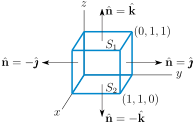
\includegraphics{cubeDT.pdf}
\end{center}
Observe that
\begin{align*}
\vF\cdot\hn = f\,\hk\cdot\hn = \begin{cases} +f &\text{on $S_1$} \\
                            -f &\text{on $S_2$} \\
                            0  &\text{on $S_3$, $S_4$, $S_5$, $S_6$}
             \end{cases}
\end{align*}
So the divergence theorem gives
\begin{align*}
\tripInt_V\frac{\partial f}{\partial z}(x,y,z)\ \dee{x}\,\dee{y}\,\dee{z}
&=\tripInt_V \vnabla\cdot\vF(x,y,z)\ \dee{x}\,\dee{y}\,\dee{z} \\
&= \dblInt_{\partial V} \vF\cdot\hn\ \dee{S}
=\sum_{j=1}^6  \dblInt_{S_j} \vF\cdot\hn\ \dee{S}\\
&=\dblInt_{S_1} f\ \dee{S}
     -\dblInt_{S_2} f\ \dee{S} \\
&=\dblInt_R f(x,y,1)\ \dee{x}\,\dee{y}
  - \dblInt_R f(x,y,0)\ \dee{x}\,\dee{y}
\end{align*}

\end{solution}

\goodbreak
%%%%%%%%%%%%%%%%%%%%%%%%%%%
\begin{question}
\begin{enumerate}[(a)]
\item
By applying the divergence theorem to $\vF=\phi\,\va$,
where $\va$ is an arbitrary constant vector, show that
\begin{equation*}
\tripInt_V \vnabla\phi\,\dee{V}=\dblInt_{\partial V}\phi\,\hn\,\dee{S}
\end{equation*}
\item 
Show that the centroid $(\bar x,\bar y,\bar z)$ of a solid $V$
with volume $|V|$ is given by
\begin{equation*}
(\bar x,\bar y,\bar z)=\frac{1}{2|V|}\dblInt_{\partial V} (x^2+y^2+z^2)\,\hn\,\dee{S}
\end{equation*}
\end{enumerate}
\end{question}

%\begin{hint} 
%
%\end{hint}

\begin{answer} 
See the solution.
\end{answer}

\begin{solution} 
(a) The divergence of $\phi\,\va$ is 
$\vnabla\cdot(\phi\,\va)
=\vnabla\phi\cdot\va+\phi\vnabla\cdot\va=\vnabla\phi\cdot\va$, since $\va$ is
constant. So, by
the divergence theorem, 
\begin{equation*}
\dblInt_{\partial V}\phi\,\va\cdot\hn\,\dee{S}
=\tripInt_V\vnabla\cdot(\phi\,\va)\ \dee{V}
=\tripInt_V \vnabla\phi\cdot\va\ \dee{V}
\implies \left[\dblInt_{\partial V}\phi\hn\,\dee{S}
         -\tripInt_V \vnabla\phi\,\dee{V}\right]\cdot\va=0
\end{equation*}
This is true for all vectors $\va$. In particular, applying this with
$\va=\hi,\hj,\hk$, we have that all three components of 
$\left[\dblInt_{\partial V}\phi\hn\,\dee{S}
         -\tripInt_V \vnabla\phi\,\dee{V}\right]$ are zero.
So 
\begin{equation*}
\dblInt_{\partial V}\phi\,\hn\,\dee{S}-\tripInt_V \vnabla\phi\,\dee{V}=0
\end{equation*}

(b) By part (a), with $\phi=x^2+y^2+z^2$ and 
$\vnabla\phi = 2x\,\hi+2y\,\hj+2z\,\hk$,
\begin{equation*}
\frac{1}{2|V|}\dblInt_{\partial V} (x^2+y^2+z^2)\,\hn\,\dee{S}
=\frac{1}{2|V|} \tripInt_V (2x\,\hi+2y\,\hj+2z\,\hk)\,\dee{V}
=(\bar x,\bar y,\bar z)
\end{equation*}
\end{solution}


%%%%%%%%%%%%%%%%%%
\subsection*{\Procedural}
%%%%%%%%%%%%%%%%%%

%%%%%%%%%%%%%%%%%%%%%%%%%%%%%%%%%%%
\begin{question}
Let $S$ be the unit sphere centered at the origin and oriented
by the outward pointing normal. If 
\begin{equation*}
\vF(x,y,z)=\big(x,y,z^2\big)
\end{equation*}
evaluate the flux of $\vF$ through $S$
\begin{enumerate}[(a)]
\item
   directly and
\item
   by applying the divergence theorem.
\end{enumerate}
\end{question}

\begin{hint} 
(b) The integral can be trivially evaluated by exploiting oddness
and the fact that $ \tripInt_V\ \dee{V}=\text{Volume}(V)$.
\end{hint}

\begin{answer} 
(a), (b) $\frac{8\pi}{3}$
\end{answer}

\begin{solution}
 (a) We'll parametrize the sphere using the spherical coordinates $\theta$ and
$\varphi$.
\begin{align*}
x&=\sin\varphi\cos\theta \\
y&=\sin\varphi\sin\theta \\
z&=\cos\varphi
\end{align*}
with $0\le\theta\le 2\pi$, $0\le\varphi\le \pi$.
Since
\begin{align*}
\Big(\frac{\partial x}{\partial\theta}\,,\,
      \frac{\partial y}{\partial\theta}\,,\,
      \frac{\partial z}{\partial\theta}\Big)
&=\big(-\sin\varphi\sin\theta\,,\,
       \sin\varphi\cos\theta\,,\,0\big)\\
\Big(\frac{\partial x}{\partial\varphi}\,,\,\frac{\partial y}{\partial\varphi}
             \,,\, \frac{\partial z}{\partial\varphi}\Big)
&=(\cos\varphi\cos\theta\,,\,\cos\varphi\sin\theta\,,\,-\sin\varphi) 
\end{align*}
(\eref{CLP317}{eq:SUdSparam}) in the CLP-4 text yields
\begin{align*}
\hn\,\dee{S}
&=\pm\Big(\frac{\partial x}{\partial\theta}\,,\,
          \frac{\partial y}{\partial\theta}\,,\,
          \frac{\partial z}{\partial\theta}\Big)
\times
\Big(\frac{\partial x}{\partial\varphi}\,,\,\frac{\partial y}{\partial\varphi}
   \,,\, \frac{\partial z}{\partial\varphi}\Big)
\ \dee{\theta}\dee{\varphi}\\
&=\pm \big(-\sin\varphi\sin\theta\,,\,
       \sin\varphi\cos\theta\,,\,0\big)
\times
(\cos\varphi\cos\theta\,,\,\cos\varphi\sin\theta\,,\,-\sin\varphi)
\ \dee{\theta}\dee{\varphi}\\
&=\pm\big(-\sin^2\varphi\cos\theta\,,\,
          -\sin^2\varphi\sin\theta\,,\,
          -\sin\varphi\cos\varphi\big)\ \dee{\theta}\dee{\varphi} \\
&=\mp \sin\varphi \big(\sin\varphi\cos\theta\,,\,
          \sin\varphi\sin\theta\,,\,
          \cos\varphi\big)\ \dee{\theta}\dee{\varphi}  \\
&=\mp \sin\varphi \big(x(\theta,\varphi)\,,\,
          y(\theta,\varphi)\,,\,
          z(\theta,\varphi)\big)\ \dee{\theta}\dee{\varphi} 
\end{align*}
To get an outward pointing normal we need the $+$ sign, since then
$\hn(\theta,\varphi)$ is a positive multiple, namely $\sin\varphi$,
times $\vr(\theta,\varphi)$. So, on $S$,
\begin{align*}
\vF\cdot\hn\,\dee{S}
  &= \sin\varphi \overbrace{\big(\sin\varphi\cos\theta\,,\,
          \sin\varphi\sin\theta\,,\,
          \cos^2\varphi\big)}^{\vF}\cdot
      \big(\sin\varphi\cos\theta\,,\,
          \sin\varphi\sin\theta\,,\,
          \cos\varphi\big)\ \dee{\theta}\dee{\varphi}   \\
  &= \sin\varphi\big(\sin^2\varphi\cos^2\theta
             +\sin^2\varphi\sin^2\theta+\cos^3\varphi\big)
\end{align*}
and
\begin{align*}
\dblInt_S\vF\cdot\hn\,\dee{S}
&=\int_0^\pi \dee{\varphi}\int_0^{2\pi}\dee{\theta}\ \sin\varphi\big(\sin^2\varphi\cos^2\theta
+\sin^2\varphi\sin^2\theta+\cos^3\varphi\big)\cr
&=\int_0^\pi \dee{\varphi}\int_0^{2\pi}\dee{\theta}\ 
      \big(\sin^3\varphi + \sin\varphi\cos^3\varphi\big)\cr
&=2\pi \left\{\int_0^\pi \dee{\varphi}\ \sin^3\varphi
         \ +\ \left[-\frac{1}{4}\cos^4\varphi\right]^\pi_0 \right\}\cr
&=2\pi\int_0^\pi \dee{\varphi}\ \sin\varphi(1-\cos^2\varphi)
=2\pi\left[-\cos\varphi+\frac{1}{3}\cos^3\varphi\right]_0^\pi
=2\pi\left[\frac{4}{3}\right] \\
&=\frac{8\pi}{3}
\end{align*}

(b) Let $V$ be the interior of $S$. Then, by the divergence theorem,
\begin{equation*}
\dblInt_S\vF\cdot\hn\,\dee{S}
=\tripInt_V\vnabla\cdot\vF\ \dee{V}
=\tripInt_V(1+1+2z)\ \dee{V}
\end{equation*}
By oddness under $z\rightarrow -z$, the $z$ integral vanishes, so that
\begin{equation*}
\dblInt_S\vF\cdot\hn\,\dee{S}
=2\tripInt_V\ \dee{V}
=2\,\text{Volume}(V)
=2\frac{4\pi}{3}
=\frac{8\pi}{3}
\end{equation*}
\end{solution}


%%%%%%%%%%%%%%%%%%%%%%%%%%%
\begin{question}
 Evaluate, by two methods, the integral 
$\dblInt_S\vF\cdot \hn\,\dee{S}$, where $\vF=z\,\hk$, 
$S$ is the surface $x^2+y^2+z^2=a^2$
and $\hn$ is the outward pointing unit normal to $S$.
\begin{enumerate}[(a)]
\item
First, by direct computation of the surface integral.
\item
Second, by using the divergence theorem.
\end{enumerate}
\end{question}

\begin{hint} 
For part (a), use spherical coordinates.
\end{hint}

\begin{answer} 
(a), (b) $\frac{4}{3}\pi a^3$
\end{answer}

\begin{solution} 
(a) Let's use spherical coordinates. As $S$ is the
sphere of radius $a$ centred on the origin,  we can parametrize it by
\begin{align*}
\vr(\theta,\varphi) 
  &=a\sin\varphi\cos\theta\,\hi
     +a\sin\varphi\sin\theta\,\hj
     + a\cos\varphi\,\hk \\
\pdiff{\vr}{\theta}
   &=-a\sin\varphi\sin\theta\,\hi
     +a\sin\varphi\cos\theta\,\hj \\
\pdiff{\vr}{\varphi}
   &= \phantom{-}a\cos\varphi\cos\theta\,\hi
     +a\cos\varphi\sin\theta\,\hj
    -a\sin\varphi\,\hk \\
\hn\,\dee{S}
&=\pm\pdiff{\vr}{\theta}
   \times \pdiff{\vr}{\varphi}
    \ \dee{\theta}\, d\varphi\\
&=\det\left[\begin{matrix}   \hi &\hj &\hk \\
              -a\sin\varphi\sin\theta & a\sin\varphi\cos\theta & 0 \\
              a\cos\varphi\cos\theta & a\cos\varphi\sin\theta & -a\sin\varphi
   \end{matrix}\right]  \dee{\theta}\, d\varphi\\
&=\pm\Big(-a^2\sin^2\varphi\cos\theta\,\hi
          -a^2\sin^2\varphi\sin\theta\,\hj
          -a^2\sin\varphi\cos\varphi\,\hk\Big)\ \dee{\theta}\, d\varphi \\
&=\mp a^2\sin\varphi \big(\sin\varphi\cos\theta\,\hi
          +\sin\varphi\sin\theta\,\hj
          +\cos\varphi\,\hk\Big)\ \dee{\theta}\, d\varphi 
\end{align*}
For the outward normal, we want the $+$ sign, so
\begin{align*}
\hn\,\dee{S}
&= a^2\sin\varphi \big(\sin\varphi\cos\theta\,\hi
          +\sin\varphi\sin\theta\,\hj
          +\cos\varphi\,\hk\Big)\ \dee{\theta}\, d\varphi  \\
\vF\cdot \hn\,\dee{S} &= z(\theta,\varphi)\,\hk\cdot \hn\,\dee{S}
           = a^3 \sin\varphi\cos^2\varphi\ \dee{\theta}\,d\varphi 
\end{align*}
and
\begin{align*}
\dblInt_S\vF\cdot \hn\,\dee{S}
&= a^3\int_0^\pi d\varphi\int_0^{2\pi}\dee{\theta}\ \sin\varphi\,\cos^2\varphi\\
&=2\pi a^3 \int_0^\pi d\varphi \ \sin\varphi\,\cos^2\varphi
=2\pi a^3\left[-\frac{1}{3}\cos^3\varphi\right]_0^\pi \\
&=\frac{4}{3}\pi a^3
\end{align*}

(b) Call the solid $x^2+y^2+z^2\le a^2$, $V$.
As
\begin{equation*}
\vnabla\cdot\vF
=\pdiff{}{x}(0)
+\pdiff{}{y}(0)
+\pdiff{}{z}(z)
=1
\end{equation*}
the divergence theorem gives
\begin{align*}
\dblInt_{\cS}\vF\cdot\hn\,\dee{S}
&=\tripInt_V\vnabla\cdot\vF\ \dee{V}
=\tripInt_V \ \dee{V}
=\text{Volume}(V)
=\frac{4}{3}\pi a^3
\end{align*}
\end{solution}

%%%%%%%%%%%%%%%%%%%%%%%%%%%
\begin{question}
 Let 
\begin{itemize}\itemsep1pt \parskip0pt \parsep0pt %\itemindent-15pt
\item
$\ \vF=zy^3\,\hi+yx\, \hj+(2z+y^2)\hk\ $ and
\item
 $V$ be the solid in 3-space defined by
$$
0\le z\le \frac{9-x^2-y^2}{9+x^2+y^2}
$$
and
\item
$D$ be the bottom surface of $V$.
Because $\frac{9-x^2-y^2}{9+x^2+y^2}$ is positive for 
$x^2+y^2< 9$ and negative for $x^2+y^2> 9$,
the bottom surface is $z=0$, $x^2+y^2\le 9$.
\item
Let $S$ be the curved portion of the boundary of $V$.
It is $z={9-x^2-y^2\over 9+x^2+y^2}$, $x^2+y^2\le 9$.
Here is a sketch of the first octant part of $S$ and $D$.
\begin{center}
       \includegraphics{divThmA.pdf}
\end{center}
\end{itemize}
Denote by $|V|$ the volume of $V$ and compute, in terms of $|V|$,
\begin{enumerate}[(a)]
\item
$\dst\dblInt_{D}\vF\cdot \hn\,\dee{S}$\quad\quad with $\hn$ pointing downward
\item
$\dst\tripInt_V\vnabla\cdot F\,\dee{V}$
\item
$\dst\dblInt_S\vF\cdot\hn\,\dee{S}$\quad\quad with $\hn$ pointing outward
\end{enumerate}
Use the divergence theorem to answer at least one of parts (a), (b) and
(c).
\end{question}

\begin{hint} 
(a) The integral is easier in polar coordinates.

(b) Since $x$ is odd, $\tripInt_V x\,\dee{V}=0$.

\end{hint}

\begin{answer}
(a) $-\frac{81}{4}\pi$\qquad 
(b) $2|V|$ \qquad
(c) $2|V|+\frac{81}{4}\pi$
\end{answer}

\begin{solution} 
(a)
On $D$, $z=0$ and
\begin{equation*}
\hn=-\hk\qquad
\dee{S}=\dee{x}\,\dee{y}\qquad 
\vF\cdot\hn=-y^2
\end{equation*}
so that
\begin{equation*}
\dblInt_{D}\vF\cdot \hn\,\dee{S}
=-\dblInt_D y^2\,\dee{x}\,\dee{y}
\end{equation*}
Switching to polar coordinates
\begin{align*}
\dblInt_{D}\vF\cdot \hn\,\dee{S}
&=-\int_0^3 dr\,r\int_0^{2\pi}\dee{\theta}\ \big(r\sin\theta\big)^2
=-\bigg[\int_0^3 dr\,r^3\bigg]\ \bigg[\int_0^{2\pi}\dee{\theta}\ \sin^2\theta\bigg]\\
&=-\frac{3^4}{4}\ \bigg[\int_0^{2\pi}\dee{\theta}\ \frac{1-\cos(2\theta)}{2}\bigg]
=-\frac{81}{4}\bigg[\frac{\theta}{2}-\frac{\sin(2\theta)}{4}\bigg]_0^{2\pi}
=-\frac{81}{4}\pi
\end{align*}
For an efficient, sneaky, way to evaluate 
$\int_0^{2\pi} \sin^2 \theta\ \dee{\theta}$, see Example
\eref{CLP317}{eg:workIntegalB} in the CLP-4 text.
% Example 2.4.4

(b)
Observe that $\vnabla\cdot \vF=x+2$. Since $x$ is odd and $V$ is invariant
under $x\rightarrow -x$, we have $\tripInt_V x\,\dee{V}=0$ (more details
below) so that
\begin{equation*}
\tripInt_V\vnabla\cdot F\,\dee{V}
=\tripInt_V (x+2)\,\dee{V}
=2\tripInt_V \,\dee{V}
=2|V|
\end{equation*}
Here are two more detailed arguments showing that $\tripInt_V x\,\dee{V}=0$.

\emph{Argument 1:} \ \ \ We may rewrite the equation 
$z=\frac{9-x^2-y^2}{9+x^2+y^2}$ of the curved boundary of $V$
as
\begin{equation*}
z(9+x^2+y^2) = 9-x^2-y^2 \iff
x^2+y^2 = \frac{9(1-z)}{1+z}
\end{equation*}
This is the equation of the circle of radius 
$r(z)=\sqrt{\frac{9(1-z)}{1+z}}$ centred on $x=y=0$.
So $z$ runs from $0$ to $1$, and for each fixed $0\le z\le 1$,
$y$ runs from  $-r(z)$ to $r(z)$
and, for each fixed $y$ and $z$, $x$ runs from $-\sqrt{r(z)^2-y^2}$
to $\sqrt{r(z)^2-y^2}$. So
\begin{align*}
\tripInt_V x\,\dee{V}
=\int_0^1 \dee{z}\int_{-r(z)}^{r(z)}\dee{y}
       \int_{-\sqrt{r(z)^2-y^2}}^{\sqrt{r(z)^2-y^2}} \dee{x}\ x
=\int_0^1 \dee{z}\int_{-r(z)}^{r(z)}\dee{y}\ 0
=0
\end{align*}
since $\int_{-a}^a x\ \dee{x}=0$ for any $a>0$.

\emph{Argument 2:} \ \ \ As we have observed above, the
curved boundary of $V$ is $x^2+y^2 = \frac{9(1-z)}{1+z}$ which
is invariant under rotations about the $z$--axis. By that symmetry, the 
centroid of $V$ lies on the $z$-axis. Recall that, for any solid $V$,
the centroid of $V$ is $(\bar x,\bar y,\bar z)$ with
\begin{equation*}
\bar x = \frac{\tripInt_V x \dee{V}}{\tripInt_V \dee{V}}\qquad
\bar y = \frac{\tripInt_V y \dee{V}}{\tripInt_V \dee{V}}\qquad
\bar z = \frac{\tripInt_V z \dee{V}}{\tripInt_V \dee{V}}
\end{equation*}
So
\begin{equation*}
\tripInt_V x\,\dee{V} = \bar x\, \text{Volume}(V) =0 \qquad\text{and}\qquad
\tripInt_V y\,\dee{V} = \bar y\,  \text{Volume}(V) =0 
\end{equation*}

(c)
By the divergence theorem,
\begin{equation*}
\tripInt_V\vnabla\cdot F\,\dee{V}
=\dblInt_{\partial V}\vF\cdot \hn\,\dee{S}
=\dblInt_S\vF\cdot \hn\,\dee{S}
+\dblInt_D\vF\cdot \hn\,\dee{S}
\end{equation*}
so that
\begin{equation*}
\dblInt_S\vF\cdot \hn\,\dee{S}
=\tripInt_V\vnabla\cdot F\,\dee{V}
-\dblInt_D\vF\cdot \hn\,\dee{S}
=2|V|+\frac{81}{4}\pi
\end{equation*}
\end{solution}

\goodbreak
%%%%%%%%%%%%%%%%%%%%%%%%%%%
\begin{question}
Evaluate the integral $\dblInt_S\vF\cdot \hn\,\dee{S}$,
where $\vF=(x,y,1)$, $S$ is the surface $z=1-x^2-y^2$ 
for $x^2+y^2\le 1$, and $\hn$ is the upward pointing normal, by two methods.
\begin{enumerate}[(a)]
\item
First, by direct computation of the surface integral.
\item
Second, by using the divergence theorem.
\end{enumerate}
\end{question}

\begin{hint} 
(a) The integral is easy in polar coordinates.

(b) The volume of the solid can be easily computed by decomposing the solid
into thin horizontal pancakes. See Section \eref{CLP101}{sec int volumes}
in the CLP-2 text.

\end{hint}

\begin{answer} 
(a), (b) $2\pi$
\end{answer}

\begin{solution} 
(a)  Let $G(x,y,z) = x^2+y^2+z$. Then the surface is $G(x,y,z)=1$
and $\vnabla G(x,y,z) = 2x\,\hi+2y\,\hj+\hk$ is upward pointing (i.e. the coefficient of $\hk$ is positive) so that,
by (\eref{CLP317}{eq:SUdSimplicit}) in the CLP-4 text, 
\begin{align*}
\hn\,\dee{S}&=\frac{\vnabla G}{\vnabla G\cdot\hk}\ \dee{x}\,\dee{y}
=\frac{2x\,\hi+2y\,\hj+\hk}{1}\,\dee{x}\,\dee{y}
=(2x\,\hi+2y\,\hj+\hk)\,\dee{x}\,\dee{y}\\
\vF\cdot\hn\,\dee{S}
&=\big[x\,\hi+y\,\hj+\hk\big]\cdot
          \big[2x\,\hi+2y\,\hj+\hk\big]\,\dee{x}\,\dee{y}
=\big[2x^2+2y^2+1\big]\,\dee{x}\,\dee{y}
\end{align*}
Switching to polar coordinates
\begin{equation*}
\dblInt_S\vF\cdot \hn\,\dee{S}
=\int_0^1dr\ r\int_0^{2\pi}\dee{\theta}\ (2r^2+1)
=2\pi\left[\frac{2}{4} r^4+\frac{1}{2} r^2\right]_0^1
=2\pi
\end{equation*}

(b) Call the solid $0\le z\le 1-x^2-y^2$, $V$.
\begin{center}
       \includegraphics{divThmB.pdf}
\end{center}
Let  $D$ denote the bottom surface of $V$.
The disk $D$ has radius $1$, area $\pi$, $z=0$ and outward normal $-\hk$, 
so that
\begin{equation*}
\dblInt_{D}\vF\cdot\hn\,\dee{S}
=-\dblInt_{D}\vF\cdot\hk\,\dee{x}\,\dee{y}
=-\dblInt_{D}\dee{x}\,\dee{y}
=-\pi
\end{equation*}
As
\begin{equation*}
\vnabla\cdot\vF
=\pdiff{}{x}(x)
+\pdiff{}{y}(y)
+\pdiff{}{z}(1)
=2
\end{equation*}
the divergence theorem gives
\begin{align*}
\dblInt_{\cS}\vF\cdot\hn\,\dee{S}
&=\tripInt_V\vnabla\cdot\vF\ \dee{V}
-\dblInt_{D}\vF\cdot\hn\,\dee{S}
=\tripInt_V 2\ \dee{V} -(-\pi)
=\pi + 2\tripInt_V \dee{V} 
\end{align*}
To evaluate the volume $\tripInt_V \dee{V}$, we slice the $V$ into
thin horizontal pancakes. Here is a sketch of the pancake at height
$z$.
\begin{center}
       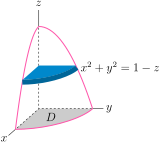
\includegraphics{divThmC.pdf}
\end{center}
Its cross-section is a circular disk of radius $\sqrt{1-z}$,
and hence of area $\pi(1-z)$. As the pancake has thickness $\dee{z}$, 
it has volume $\pi(1-z)\,\dee{z}$. So
\begin{align*}
\dblInt_{\cS}\vF\cdot\hn\,\dee{S}
&=\pi+2\int_0^1 \dee{z}\dblInt_{x^2+y^2\le 1-z} \dee{x}\,\dee{y}
=\pi+2\int_0^1 \dee{z}\ \pi(1-z)\\
&=\pi+2\pi\left[z-\frac{1}{2}z^2\right]_0^1
=2\pi
\end{align*}
\end{solution}

%%%%%%%%%%%%%%%%%%%%%%%%%%%%%%%%%%%
\begin{question}[M317 2012D] %7

\begin{enumerate}[(a)]
\item
Find the divergence of the vector field $\vF = (z + \sin y, zy, \sin x \cos y)$.
\item
Find the flux of the vector field $\vF$ of (a) outward through the sphere of 
radius $3$ centred at the origin in $\bbbr^3$ .
\end{enumerate}
\end{question}

\begin{hint} 
The divergence theorem, of course.
\end{hint}

\begin{answer} 
(a) $z$\qquad
(b) $0$
\end{answer}

\begin{solution} (a)
The divergence is
\begin{align*}
\vnabla\cdot\vF &= 
    \pdiff{}{x}\big(z+\sin y\big)
     +\pdiff{}{y}\left(zy\right)
     +\pdiff{}{z}\big(\sin x\cos y\big) \\
   &=   z
\end{align*}

\noindent (b) Let
\begin{align*}
V=\Set{(x,y,z)}{x^2+y^2+z^2\le 9}
\end{align*}
By the divergence theorem (note that we are to find the \emph{outward} 
flux),
\begin{align*}
\dblInt_{\partial V}  \vF\cdot\hn\,\dee{S}
&= \tripInt_V \vnabla\cdot \vF\ \dee{V} 
= \tripInt_V z\ \dee{V} 
= 0
\end{align*}
since $z$ is odd.
\end{solution}

%%%%%%%%%%%%%%%%%%%%%%%%%%%%%%%%%%%
\begin{question}
The sides of a grain silo are described by the portion of the 
cylinder $x^2 + y^2 = 1$ with $0 \le z\le 1$. The top of the silo is 
given by the portion of the sphere $x^2+ y^2+ z^2 = 2$ lying within the 
cylinder and above the $xy$-plane. Find the flux of the vector field
\begin{equation*}
\vV(x,y,z) = (x^2yz\,,\, yz+e^xz\,,\, x^2+y ) 
\end{equation*}
out of the silo. 
\end{question}

\begin{hint}
It's easier to use the divergence theorem.
But don't forget the base of the silo. 
\end{hint}

\begin{answer} 
$\pi$
\end{answer}

\begin{solution} 
Call the silo $V$.
Call the sides and top of the silo $S$. Call the base of the silo (namely,
$x^2+y^2\le 1$, $z=0$) $B$. By the divergence theorem,
\begin{align*}
\dblInt_S \vV\cdot\hn\ \dee{S} + \dblInt_B \vV\cdot(-\hk)\ \dee{S}
&=\tripInt_V\vnabla\cdot\vV\ \dee{V}\\
\dblInt_S \vV\cdot\hn\ \dee{S} 
        - \dblInt_{x^2+y^2\le 1} (x^2+y)\ \dee{x}\,\dee{y}
&=\tripInt_V(2xyz+z)\ \dee{V}\\
\end{align*}
By oddness under $Y\rightarrow -y$,
 $\dblInt_{x^2+y^2\le 1} y\ \dee{x}\,\dee{y} 
        = \tripInt_V xyz\ \dee{V}=0$, so
\begin{align*}
\dblInt_S \vV\cdot\hn\ \dee{S}
&=\dblInt_{x^2+y^2\le 1} x^2\ \dee{x}\,\dee{y} +\tripInt_V z\ \dee{V} \\
&=\int_0^1 \dee{r}\int_0^{2\pi}\dee{\theta}\ r\ (\overbrace{r\cos\theta}^{x})^2 
           +\tripInt_V z\ \dee{V}
\end{align*}
We can evaluate the volume integral by decomposing $V$
into thin horizontal pancakes. See Section \eref{CLP101}{sec int volumes}
in the CLP-2 text.
For $0\le z\le 1$, the horizontal cross-section of the silo at height
$z$ is a circle of radius $1$ and hence of area $\pi$. For $z\ge1$,
the horizontal cross-section of the silo at height $z$ is again a 
circle. Its radius is determined by the equation $x^2+ y^2+ z^2 = 2$ of
the top of the silo. The radius is $\sqrt{2-z^2}$, so the cross-section
has area $\pi(2-z^2)$. The biggest that $z$ can get is $\sqrt{2}$. Thus
\begin{align*}
\dblInt_S \vV\cdot\hn\ \dee{S}
&=\int_0^1 \dee{r}\int_0^{2\pi}\dee{\theta} \ r\ (r\cos\theta)^2+\int_0^1 dz\ \pi z
+\int_1^{\sqrt{2}}dz\ \pi(2-z^2) z\\
&=\left[\int_0^1 \dee{r}\ r^3\right]
   \left[\int_0^{2\pi}\dee{\theta} \ \frac{\cos(2\theta)+1}{2}\right]+\int_0^1 dz\ \pi z
+\int_1^{\sqrt{2}}dz\ \pi(2-z^2) z\\
&=\left[\frac{r^4}{4}\right]_0^1\pi
 +\left[\pi\frac{z^2}{2}\right]_0^1
 +\pi\left[z^2-\frac{z^4}{4}\right]_1^{\sqrt{2}}\\
&=\frac{\pi}{4}+\frac{\pi}{2}+\pi\left[1-\frac{3}{4}\right]\\
&=\pi
\end{align*}
For an efficient, sneaky, way to evaluate 
$\int_0^{2\pi} \cos^2 \theta\ \dee{\theta}$, see Example
\eref{CLP317}{eg:workIntegalB} in the CLP-4 text.
\end{solution}

%%%%%%%%%%%%%%%%%%%%%%%%%%%%%%%%%%%
\begin{question}
Let $B$ be the ball of volume $V$ centered at the point 
$(x_0, y_0, z_0)$, and let $S$ be the sphere that is the boundary of $B$.  
Find the flux of $\vF = x^2\hi + xy\hj+(3 z - yz)\hk$ outward (from $B$) 
through $S$. 
\end{question}

\begin{hint} 
The divergence theorem, of course.
The integral can be easily evaluated by using that, 
for any solid $\cV$ in $\bbbr^3$,
\begin{align*}
\tripInt_\cV\dee{V}=\text{Volume}(\cV)\qquad
\bar x =\frac{\tripInt_\cV x\,\dee{V}}{\text{Volume}(\cV)}\qquad
\bar y =\frac{\tripInt_\cV y\,\dee{V}}{\text{Volume}(\cV)}\qquad
\bar z =\frac{\tripInt_\cV z\,\dee{V}}{\text{Volume}(\cV)}
\end{align*}
where $(\bar x,\bar y,\bar z)$ is the centroid of $\cV$.
\end{hint}

\begin{answer} 
$[3+3x_0-y_0]\,V$
\end{answer}

\begin{solution}
Apply the divergence theorem.  The divergence of $\vF$ is
\begin{equation*}
\vnabla\cdot\vF = \pdiff{}{x}(x^2)
+\pdiff{}{y}(xy)
+\pdiff{}{z}(3 z - yz)
=3+3x-y
\end{equation*}
So
\begin{align*}
\dblInt_S\vF\cdot\hn\,\dee{S}
=\tripInt_B\vnabla\cdot\vF\ \dee{V}
=\tripInt_B(3+3x-y)\ \dee{V}
\end{align*}
To evaluate the integrals of $x$ and $y$ we use that, for any solid $\cV$
in $\bbbr^3$,
\begin{align*}
\tripInt_\cV\dee{V}=\text{Volume}(\cV)\qquad
\bar x =\frac{\tripInt_\cV x\,\dee{V}}{\text{Volume}(\cV)}\qquad
\bar y =\frac{\tripInt_\cV y\,\dee{V}}{\text{Volume}(\cV)}\qquad
\bar z =\frac{\tripInt_\cV z\,\dee{V}}{\text{Volume}(\cV)}
\end{align*}
where $(\bar x,\bar y,\bar z)$ is the centroid of $\cV$.
Our ball has volume $V$ and centroid
$(\bar x,\bar y,\bar z) = (x_0,y_0,z_0)$.
So
\begin{align*}
\dblInt_S\vF\cdot\hn\,\dee{S}
= V[3+3\bar x-\bar y]
=[3+3x_0-y_0]\,V
\end{align*}
\end{solution}




%%%%%%%%%%%%%%%%%%%%%%%%%%%
\begin{question}[M317 2010D] %7
Let
\begin{equation*}
\vF(x, y, z) = \big( 1 + z^{1+z^{1+z}}\,,\, 1 + z^{1+z^{1+z}}\,,\,1\big)
\end{equation*} 
Let $S$ be the portion of the surface
\begin{equation*}
x^2 + y^2 = 1 - z^4
\end{equation*}
which is above the $xy$-plane. What is the flux of $\vF$ downward through $S$?
\end{question}

\begin{hint} 
The complexity of $\vF$ is a hint that the flux should
not be evaluated directly.
\end{hint}

\begin{answer} 
$-\pi$
\end{answer}

\begin{solution} Let
\begin{equation*}
V=\Set{(x,y,z)}{x^2+y^2\le 1-z^4,\ 0\le z\le 1}
\end{equation*}
Then the boundary, $\partial V$, of $V$, with the orientation
that is used in the divergence theorem, consists of two parts
\begin{itemize}
\item
the surface $S$, but with the upward pointing normal, and 
\item
the disk $D=\Set{(x,y,z)}{x^2+y^2\le 1,\ z=0}$, with normal $-\hk$.
\end{itemize}
So the divergence theorem gives
\begin{align*}
\tripInt_V \vnabla\cdot\vF\,\dee{V}
=\dblInt_{\partial V}\vF\cdot\hn\,\dee{S}
=- \dblInt_S\vF\cdot\hn\,\dee{S}
  +\dblInt_D\vF\cdot(-\hk)\,\dee{S}
\end{align*}
As $\vnabla\cdot\vF=0$ and $\vF(x,y,0) = \big( 1 \,,\, 1 \,,\,1\big)$
\begin{align*}
\dblInt_S\vF\cdot\hn\,\dee{S}
=\dblInt_D\vF\cdot(-\hk)\,\dee{S}
=-\dblInt_D\dee{S}
=-\pi
\end{align*}


\end{solution}

%%%%%%%%%%%%%%%%%%%%%%%%%%%
\begin{question}[M317 2002A] %5
Use the divergence theorem to find the flux of $x\hi+y\hj+2z\hk$
through the part of the ellipsoid 
$$
x^2+y^2+2z^2=2
$$
with $z\ge 0$. [Note: the ellipsoid $\frac{x^2}{a^2}+\frac{y^2}{b^2}+\frac{z^2}{c^2}=1$
has volume $\frac{4}{3}\pi abc$.]
\end{question}

\begin{hint} 
The specified surface is not closed.
\end{hint}

\begin{answer} 
$\frac{16}{3}\pi$
\end{answer}

\begin{solution} 
 Let $V$ be the solid $x^2+y^2+2z^2\le 2$,
$z\ge 0$. The surface of $V$ consists of the half-ellipsoid
$S=\Set{(x,y,z)}{x^2+y^2+2z^2=2,\ z\ge 0}$, on top with upward pointing normal,
and the disk $D=\set{(x,y,z)}{z=0,\ x^2+y^2\le 2}$, on the bottom with 
normal $-\hk$.
Call the vector field $\vF$. By the divergence theorem
$$
\dblInt_S\vF\cdot\hn\ \dee{S}
+\dblInt_D\vF\cdot(-\hk)\,\dee{S}
=\tripInt_V\vnabla\cdot\vF\ \dee{V}
=\tripInt_V 4\ \dee{V}
$$
The ellipsoid has $a=\sqrt{2}$, $b=\sqrt{2}$, $c=1$ and volume 
$\frac{4}{3}\pi abc=\frac{8}{3}\pi$. So 
$$
\tripInt_V 4\ \dee{V}=4\times\half({\rm Volume\ of\ the\ ellipsoid})=\frac{16\pi}{3}
$$
On $D$, $z=0$ and $\dblInt_D x\,\dee{S}=\dblInt_D y\,\dee{S}=0$
because $x$ and $y$ are odd.
So
$$
\dblInt_D\vF\cdot(-\hk)\,\dee{S}
=\dblInt_D(x\hi+y\hj+0\hk)\cdot(-\hk)\,\dee{S}
=0
$$
and the desired flux is 
$$
\dblInt_S\vF\cdot\hn\ \dee{S}=\tripInt_V 4\ \dee{V}
=\frac{16}{3}\pi
$$
\end{solution}

%%%%%%%%%%%%%%%%%%%%%%%%%%%
\begin{question}[M317 2010A] %4
Let $\vF(x,y,z) = \vr/r^3$ where $\vr= x\,\hi + y\,\hj + z\,\hk$ and 
$r = |\vr|$.
\begin{enumerate}[(a)]
\item
Find $\vnabla \cdot \vF$.
\item
Find the flux of $\vF$ outwards through the spherical surface 
$x^2 + y^2 + z^2 = a^2$.
\item
Do the results of (a) and (b) contradict the divergence theorem? Explain your
answer.
\item
Let $E$ be the solid region bounded by the surfaces 
$z^2 - x^2 - y^2 + 1 = 0$, $z = 1$ and $z = -1$. Let $\sigma$ be 
the bounding surface of $E$. Determine the flux of $\vF$
outwards through $\sigma$.
\item
Let $R$ be the solid region bounded by the surfaces
$z^2 - x^2 - y^2 + 4y - 3 = 0$, $z = 1$ and $z = - 1$. Let $\Sigma$ 
be the bounding surface of $R$. Determine the flux of $\vF$ 
outwards through $\Sigma$.
\end{enumerate}
\end{question}

\begin{hint} 
(a), (b), (c) Review warning \eref{CLP317}{warn:divThm} in the CLP-4 text.

(d) The divergence theorem can be used --- with care.

(e) The equation can be made more understandable by completing a square.
\end{hint}

\begin{answer} 
(a) $\vnabla \cdot \vF(x,y,z)=0$ except at $(x,y,z)=(0,0,0)$, where
$\vF$ is not defined.

(b) $4\pi$\qquad
(c) No. \qquad
(d) $4\pi$\qquad
(e) $0$

\end{answer}

\begin{solution} (a) 
If $(x,y,z)\ne\vZero$,
\begin{align*}
&\vnabla\cdot\vF(x,y,z)
=\pdiff{}{x}\frac{x}{{\big[x^2+y^2+z^2\big]}^{3/2}}
+\pdiff{}{y}\frac{y}{{\big[x^2+y^2+z^2\big]}^{3/2}}
+\pdiff{}{z}\frac{z}{{\big[x^2+y^2+z^2\big]}^{3/2}}
\\
&\hskip0.25in
=\frac{\big[x^2+y^2+z^2\big]-x\frac{3}{2}(2x)}{{\big[x^2+y^2+z^2\big]}^{5/2}}
+\frac{\big[x^2+y^2+z^2\big]-y\frac{3}{2}(2y)}{{\big[x^2+y^2+z^2\big]}^{5/2}}
+\frac{\big[x^2+y^2+z^2\big]-z\frac{3}{2}(2z)}{{\big[x^2+y^2+z^2\big]}^{5/2}}
\\
&\hskip0.25in
=\frac{3\big[x^2+y^2+z^2\big]-3x^2-3y^2-3z^2}{{\big[x^2+y^2+z^2\big]}^{5/2}}
=0
\end{align*}
If $(x,y,z)=\vZero$, $\vF(x,y,z)$ is not defined 
and hence $\vnabla\cdot\vF(x,y,z)$ is also not defined.

\noindent (b)
Let $a>0$. Write
$\sigma_a = \Set{(x,y,z)}{x^2+y^2+z^2 = a^2}$. The outward unit normal 
to $\sigma_a$ is $\hn = \frac{\vr}{|\vr|}$ so that
\begin{align*}
\int_{\sigma_a}\vF\cdot\hn\, \dee{S}
&=\int_{|\vr|=a}  \frac{\vr}{|\vr|^3}\cdot \frac{\vr}{|\vr|}\ \dee{S} 
=\int_{|\vr|=a}  \frac{1}{|\vr|^2}\ \dee{S}
=\frac{1}{a^2}\int_{|\vr|=a}\dee{S} 
=\frac{1}{a^2}\big(4\pi a^2\big) \\
&=4\pi\ne 0
\end{align*}

\noindent (c)
No, the results of (a) and (b) do not contradict the divergence theorem.
One hypothesis of the divergence theorem is that $\vnabla\cdot\vF$
(in fact all first order derivatives of $\vF$) be defined and continuous
throughout the solid that $\vnabla\cdot\vF$ is to be integrated over.
That hypothesis is violated in this case.

\noindent (d)
Let's first figure out what the surface $z^2 - x^2 - y^2 + 1 = 0$,
i.e. the surface $x^2 + y^2 = 1 +z^2$, looks like. For each $z_0$, the
$z=z_0$ cross-section of this surface is the circle $x^2+y^2=1+z_0^2$.
The radius of this circle is $1$ when $z_0=0$ and grows as $|z_0|$
increases. So the solid region $E$ looks like an hourglass drum, as sketched
in the figure on the left below.

\begin{center}
  \raisebox{-8pt}[108pt][0pt]{\includegraphics[scale=1.2]{hyperboloid1.pdf}}
       \qquad\qquad
       \raisebox{-25pt}[0pt][23pt]{\includegraphics{hyperboloidHole.pdf}}
\end{center}

We are going to use the divergence theorem to compute the flux of $\vF$
out through the surface $\sigma$ of $E$. However we cannot apply the
divergence theorem using $E$ as the solid, because $\vF$ is not defined
at the origin, $(0,0,0)$, which is a point in $E$. So we pick any 
$0<a<1$, and define the auxiliary solid
\begin{equation*}
E_a = \Set{(x,y,z)}{ x^2+y^2+z^2\ge a^2,\ 
                    x^2+y^2\le 1+z^2,\ 
                    -1\le z\le 1}
\end{equation*}
The solid $E_a$ is constructed from the solid $E$ by removing 
the ball $x^2+y^2+z^2\le a^2$ from it. A side view of $E_a$ is sketched 
in the figure on the right above. As in part (b), denote by $\sigma_a$
the surface $x^2+y^2+z^2=a^2$ with \emph{outward} pointing normal.
Then the boundary of $E_a$ is $\partial E_a=\sigma-\sigma_a$, meaning that 
it consists of two parts. One part is the boundary, $\sigma$, of $E$,
with outward pointing normal. The other part is the surface 
$x^2+y^2+z^2=a^2$, but with normal pointing into the sphere, opposite to the
normals for $\sigma_a$. Consequently the divergence theorem gives
\begin{align*}
0=\tripInt_{E_a} \vnabla \cdot \vF\,\dee{V}
 =\dblInt_{\partial E_a} \vF\cdot\hn\,\dee{S}
 = \dblInt_{\sigma} \vF\cdot\hn\,\dee{S}
      -\dblInt_{\sigma_a} \vF\cdot\hn\,\dee{S}
\end{align*}
so that, by part (b)
\begin{align*}
\dblInt_{\sigma} \vF\cdot\hn\,\dee{S}
=\dblInt_{\sigma_a} \vF\cdot\hn\,\dee{S}
=4\pi
\end{align*}

\noindent (e) 
The equation $z^2 - x^2 - y^2 + 4y - 3 = 0$ can be rewritten as
\begin{equation*}
x^2 + (y-2)^2 = 1+z^2
\end{equation*}
As is part (d), for each $z_0$, the
$z=z_0$ cross-section of this surface is a circle $x^2+(y-2)^2=1+z_0^2$
of radius $\sqrt{1+z_0^2}$. But this circle is centred at
$(0,2,z_0)$, whereas the corresponding circle in part (d) was centred at
$(0,0,z_0)$. The solid $R$ again has the shape of an hourglass drum.
But while the origin $(0,0,0)$ was in $E$, it is \emph{not} in
\begin{equation*}
R=\Set{(x,y,z)}{x^2+(y-2)^2\le 1+z^2,\ -1\le z\le 1}
\end{equation*}
So $\vnabla \cdot \vF=0$ \emph{throughout all} of $R$ and the
divergence theorem gives
\begin{align*}
\dblInt_{\Sigma} \vF\cdot\hn\,\dee{S}
=\dblInt_{\partial R} \vF\cdot\hn\,\dee{S}
=\tripInt_{R} \vnabla \cdot \vF\,\dee{V}
=0
\end{align*}
\end{solution}

%%%%%%%%%%%%%%%%%%%%%%%%%%%
\begin{question}[M317 2009A] %6
Consider the ellipsoid $S$ given by
\begin{equation*}
x^2 + \frac{y^2}{4} +\frac{z^2}{4} = 1
\end{equation*}
with the unit normal pointing outward.

\begin{enumerate}[(a)]
\item
Parameterize $S$.
\item
Compute the flux $\dblInt_S \vF\cdot\hn\, \dee{S}$ of the vector field
\begin{equation*}
\vF(x,y,z) = (x, y, z)
\end{equation*}
\item
Verify your answer in (b) using the divergence theorem.
\end{enumerate}
\end{question}

\begin{hint} 
(a) Use a suitable modification of spherical coordinate. 
Do not forget to specify the range of the parameters.
\end{hint}

\begin{answer} 
(a) $\vr(\theta,\varphi)
=\sin\varphi\cos\theta\,\hi
  +2\sin\varphi\sin\theta\,\hj
  +2\cos\varphi\,\hk\qquad
0\le\theta<2\pi,\ 0\le \varphi \le \pi$

(b) $16\pi$\qquad
(c) $16\pi$, again

\end{answer}

\begin{solution} (a)
If the surface were the sphere $x^2+y^2+z^2=1$, we could parametrize 
it using the spherical coordinates  $\theta$ and $\varphi$ (with the radial 
spherical coordinate $\rho=1$).
\begin{align*}
x&=\sin\varphi\cos\theta \\
y&=\sin\varphi\sin\theta \\
z&=\cos\varphi
\end{align*}
with $0\le\theta<2\pi$, $0\le \varphi \le \pi$. Our surface is not a sphere,
but the equation looks like the equation of the sphere with the units of the
$y$- and $z$-coordinates changed. In particular, if we define $\tilde y =y/2$
and $\tilde z =z/2$, so that $y=2\tilde y$ and $z=2\tilde z$, then on our
surface
\begin{align*}
1=x^2 + \frac{y^2}{4} +\frac{z^2}{4} 
 =x^2 + \frac{(2\tilde y)^2}{4} +\frac{(2\tilde z)^2}{4}
 =x^2+\tilde y^2 +\tilde z^2 
\end{align*}
and we can parametrize
\begin{align*}
x&=\sin\varphi\cos\theta \\
\tilde y&=\sin\varphi\sin\theta \\
\tilde z&=\cos\varphi
\end{align*}
and then
\begin{align*}
x&=\sin\varphi\cos\theta \\
y&=2\tilde y=2\sin\varphi\sin\theta \\
z&=2\tilde z=2\cos\varphi
\end{align*}
or
\begin{align*}
\vr(\theta,\varphi)
=\sin\varphi\cos\theta\,\hi
  +2\sin\varphi\sin\theta\,\hj
  +2\cos\varphi\,\hk\qquad
0\le\theta<2\pi,\ 0\le \varphi \le \pi
\end{align*}

\noindent (b) Considering part (c) in this question, we are presumably
to evaluate the flux integral directly.
Since
\begin{align*}
\Big(\frac{\partial x}{\partial\theta}\,,\,
      \frac{\partial y}{\partial\theta}\,,\,
      \frac{\partial z}{\partial\theta}\Big)
&=\big(-\sin\varphi\sin\theta\,,\,
       2\sin\varphi\cos\theta\,,\,0\big)\\
\Big(\frac{\partial x}{\partial\varphi}\,,\,\frac{\partial y}{\partial\varphi}
             \,,\, \frac{\partial z}{\partial\varphi}\Big)
&=(\cos\varphi\cos\theta\,,\,2\cos\varphi\sin\theta\,,\,-2\sin\varphi) 
\end{align*}
(\eref{CLP317}{eq:SUdSparam}) in the CLP-4 text yields
\begin{align*}
\hn\,\dee{S}
&=\pm\Big(\frac{\partial x}{\partial\theta}\,,\,
          \frac{\partial y}{\partial\theta}\,,\,
          \frac{\partial z}{\partial\theta}\Big)
\times
\Big(\frac{\partial x}{\partial\varphi}\,,\,\frac{\partial y}{\partial\varphi}
   \,,\, \frac{\partial z}{\partial\varphi}\Big)
\ \dee{\theta}\dee{\varphi}\\
&=\pm \big(-\sin\varphi\sin\theta\,,\,
       2\sin\varphi\cos\theta\,,\,0\big)
\times
(\cos\varphi\cos\theta\,,\,2\cos\varphi\sin\theta\,,\,-2\sin\varphi)
\ \dee{\theta}\dee{\varphi}\\
&=\pm\big(-4\sin^2\varphi\cos\theta\,,\,
          -2\sin^2\varphi\sin\theta\,,\,
          -2\sin\varphi\cos\varphi\Big)\ \dee{\theta}\dee{\varphi} \\
&=\mp 2\sin\varphi \big(2\sin\varphi\cos\theta\,,\,
          \sin\varphi\sin\theta\,,\,
          \cos\varphi\Big)\ \dee{\theta}\dee{\varphi} 
\end{align*}
To get an outward pointing normal we need the $+$ sign. For example, with the
$+$ sign, the $z$-component is $2\sin\varphi\cos\varphi
=\sin(2\varphi)$ so that the normal is pointing upward when
$0<\varphi<\frac{\pi}{2}$, i.e. in the northern hemisphere,
and is pointing downward when $\frac{\pi}{2}<\varphi<\pi$, i.e.
in the southern hemisphere. So
\begin{align*}
\vF\cdot\hn\dee{S} 
&=\big\{
     (\sin\varphi\cos\theta)(4\sin^2\varphi\cos\theta)
     + (2\sin\varphi\sin\theta)(2\sin^2\varphi\sin\theta) \\&\hskip3in
     + (2\cos\varphi)(2\sin\varphi\cos\varphi)
  \big\}\dee{\theta}\dee{\varphi} \\
&=\big\{4\sin^3\varphi\cos^2\theta
  +4\sin^3\varphi\sin^2\theta
  +4\sin\varphi\cos^2\varphi\big\}\dee{\theta}\dee{\varphi} \\
 &=4\sin\varphi \big(\sin^2\varphi +\cos^2\varphi\big)
                \dee{\theta}\dee{\varphi}\\
 &=4\sin\varphi\,\dee{\theta}\dee{\varphi}
\end{align*}
and the flux is
\begin{align*}
\dblInt_S \vF\cdot\hn\, \dee{S}
&=\int_0^\pi\dee{\varphi}\int_0^{2\pi}\dee{\theta}\ 4\sin\varphi
 =8\pi \int_0^\pi \dee{\varphi}\ \sin\varphi
=16\pi
\end{align*}

\noindent (c)
Set
\begin{equation*}
V=\Set{(x,y,z)} {x^2 + \tfrac{y^2}{4} +\tfrac{z^2}{4} \le 1}
\end{equation*}
Since $\vnabla\cdot\vF=3$, the divergence theorem gives
\begin{align*}
\dblInt_S \vF\cdot\hn\, \dee{S}
&=\tripInt_V \vnabla\cdot\vF\ \dee{V}
= 3 \text{Volume}(V)
\end{align*}
The volume contained in the ellipsoid, 
$\frac{x^2}{a^2} + \frac{y^2}{b^2} +\tfrac{z^2}{c^2}=1$, of semiaxes
$a$, $b$ and $c$ is $\frac{4}{3}\pi abc$. In our case $a=1$, $b=c=2$,
so 
\begin{align*}
\dblInt_S \vF\cdot\hn\, \dee{S}
&= 3 \text{Volume}(V)
=3\times \frac{4}{3}\pi (1)(2)(2)
=16\pi
\end{align*}
which is exactly what we found in part (b).

The volume of the ellipsoid $V$ can also be found by observing that,
in $V$,
\begin{itemize}\itemsep1pt \parskip0pt \parsep0pt %\itemindent-15pt
\item
$x$ runs from $-1$ to $1$ and
\item for each fixed $-1\le x\le 1$, $(y,z)$ runs over the
   disk $y^2+z^2\le 4(1-x^2)$, which has area $4\pi (1-x^2)$.
\end{itemize}
That is
\begin{equation*}
V=\Set{(x,y,z)} {-1\le x\le 1,\  y^2+z^2 \le 4(1-x^2)}
\end{equation*}
so that
\begin{align*}
\text{Volume}(V) &=\int_{-1}^1 \dee{x}
           \dblInt_{y^2+z^2 \le 4(1-x^2)}\dee{y}\,\dee{z} \\
&= \int_{-1}^1 \dee{x}\ 4\pi(1-x^2)
  =2\times 4\pi \int_0^1 \dee{x}\ (1-x^2)
  =8\pi\left[1-\frac{1}{3}\right] \\
&=\frac{16\pi}{3}
\end{align*}

\end{solution}

%%%%%%%%%%%%%%%%%%%%%%%%%%%
\begin{question}[M317 2009A]  %8
Evaluate the flux integral
$\dblInt_S \vF\cdot\hn\, \dee{S}$, where
\begin{equation*}
  \vF(x,y,z) = \big(x^3 + \cos(y^2)\,,\, y^3 + ze^x\,,\, z^2 + \arctan(xy)\big) 
\end{equation*}
and $S$ is the surface of the solid region bounded by the cylinder 
$x^2 + y^2 = 2$ and the planes $z = 0$ and $z = 2x + 3$. 
The surface is positively oriented (its unit normal points outward).
\end{question}

\begin{hint} 
Don't evaluate the flux directly.
\end{hint}

\begin{answer} 
$40\pi$
\end{answer}

\begin{solution} 
Set
\begin{equation*}
V=\Set{(x,y,z)}{x^2+y^2\le 2,\ 0\le z\le 2x+3}
\end{equation*}
Let's try the divergence theorem. Since
\begin{align*}
\vnabla\cdot\vF &= 
    \pdiff{}{x}\big(x^3 + \cos(y^2)\big)
     +\pdiff{}{y}\big(y^3 + ze^x\big)
     +\pdiff{}{z}\big(z^2 + \arctan(xy)\big) \\
   &=3x^2+3y^2+2z
\end{align*}
the divergence theorem (Theorem \eref{CLP317}{thm:divThm} of the CLP-4 text) 
gives
\begin{align*}
\dblInt_S \vF \cdot \hn\,\dee{S}
&=\tripInt_V \vnabla\cdot\vF\,\dee{V} \\
&=\int_{x^2+y^2\le 2}\dee{x}\dee{y}\int_0^{2x+3}\dee{z}\ 
      \big(3x^2+3y^2+2z\big) \\
&= \int_{x^2+y^2\le 2}\dee{x}\dee{y}\ 
      \big\{3(x^2+y^2)(2x+3)+(2x+3)^2\big\} \\
&= \int_{x^2+y^2\le 2}\dee{x}\dee{y}\ 
      \big\{9+12x+13x^2+9y^2+6x^3+6xy^2\big\} \\
&= 9(2\pi) +\int_{x^2+y^2\le 2}\dee{x}\dee{y}\ 
      \big\{13x^2+9y^2\big\} 
\end{align*}
because $12x$, $6x^3$ and $6xy^2$ are all odd under $x\rightarrow -x$.
To evaluate the final remaining integral, let's switch to polar coordinates.
\begin{align*}
\dblInt_{x^2+y^2\le 2} \big\{13x^2+9y^2\big\}\,\dee{x}\dee{y}
&=\int_0^{\sqrt{2}}\dee{r}\ r\int_0^{2\pi}\dee{\theta}\  
\big\{13\big(r\cos\theta)^2+9\big(r\sin\theta)^2\big\} \\
&=\int_0^{\sqrt{2}} \dee{r}\ r^3\int_0^{2\pi}\dee{\theta}\
\big\{ 13\cos^2\theta+9\sin^2\theta\big\}
\end{align*}
Since
\begin{align*}
\int_0^{2\pi}\cos^2\theta\ \dee{\theta}
&=\int_0^{2\pi}\frac{\cos(2\theta)+1}{2}\ \dee{\theta}
=\left[\frac{\sin(2\theta)}{4}+\frac{\theta}{2}\right]_0^{2\pi}
=\pi
\\
\int_0^{2\pi}\sin^2\theta\ \dee{\theta}
&=\int_0^{2\pi}\frac{1-\cos(2\theta)}{2}\ \dee{\theta}
=\left[\frac{\theta}{2}-\frac{\sin(2\theta)}{4}\right]_0^{2\pi}
=\pi
\end{align*}
we finally have
\begin{equation*}
\dblInt_S \vF \cdot \hn\,\dee{S}
=18\pi+\frac{(\sqrt{2})^4}{4}\pi\big\{13+9\big\}
=(18+22)\pi=40\pi
\end{equation*}
For an efficient, sneaky, way to evaluate 
$\int_0^{2\pi} \cos^2\theta\,\dee{\theta}$ 
and $\int_0^{2\pi} \sin^2\theta\,\dee{\theta}$,
see Example
\eref{CLP317}{eg:workIntegalB} in the CLP-4 text.

\end{solution}

%%%%%%%%%%%%%%%%%%%%%%%%%%%
\begin{question}[M317 2008D] %8
Find the flux of the vector field $(x + y, x + z, y + z)$ 
through the cylindrical surface whose equation is $x^2 + z^2 = 4$, 
and which extends from $y = 0$ to $y = 3$. (Only the curved part 
of the cylinder is included, not the two disks bounding it on the 
left and right.) The orientation of the surface is outward, 
i.e., pointing away from the $y$-axis.
\end{question}

\begin{hint} 
For practice, try doing this question twice --- once using the divergence
theorem and once using direct evaluation.
% Do not compute the integral directly.
\end{hint}

\begin{answer} 
$24\pi$
\end{answer}

\begin{solution} 
\emph{Solution 1 (divergence theorem)}:\ \ \ 
Set $\vF = (x + y, x + z, y + z)$.
Then $\vnabla\cdot\vF = 2$. That's really simple. So let's
try using the divergence theorem.

\begin{itemize}\itemsep1pt \parskip0pt \parsep0pt %\itemindent-15pt
\item[$\circ$]
Set $S=\Set{(x,y,z)}{x^2+z^2=4,\ 0\le y\le 3}$. We are to compute
$\dblInt_S\vF\cdot\hn\,\dee{S}$, with $\hn$ denoting the outward normal to $S$.
$S$ is \emph{not} the boundary of a solid, so we cannot compute
$\dblInt_S\vF\cdot\hn\,\dee{S}$ by applying the divergence theorem directly.
The figure on the left below shows the part of $S$ that is in the first octant.

\begin{center}
       \includegraphics{cylinder.pdf}\qquad
       \includegraphics{cylinder2.pdf}
\end{center}


\item[$\circ$]
On the other hand $S$, is ``almost'' the boundary of 
\begin{equation*}
V = \Set{(x,y,z)}{x^2+z^2\le 4,\ 0\le y\le 3}
\end{equation*} 
The boundary, $\partial V$ of $V$ consists of three pieces --- $S$ and the
two disks
\begin{equation*}
D_l = \Set{(x,y,z)}{x^2+z^2\le 4,\ y=0}\qquad
D_r = \Set{(x,y,z)}{x^2+z^2\le 4,\ y=3}
\end{equation*}
The figure on the right above shows the parts of $S$, $V$, $D_l$ 
and $D_r$ that are  in the first octant.
\end{itemize}
The outward normal to $D_r$ is $\hj$ and the outward normal to $D_l$ is
$-\hj$, to the divergence theorem gives
\begin{align*}
\tripInt_V \vnabla\cdot \vF\,\dee{V}
&=\dblInt_{\partial V}\vF\cdot\hn\,\dee{S} \\
&=\dblInt_{S}\vF\cdot\hn\,\dee{S}
  + \dblInt_{D_r}\vF\cdot\hj\,\dee{S}
  + \dblInt_{D_l}\vF\cdot(-\hj)\,\dee{S}
\end{align*}
Since $\vnabla\cdot\vF = 2$ and $\vF\cdot\hj = x+z$, 
\begin{align*}
\dblInt_{S}\vF\cdot\hn\,\dee{S}
&= \tripInt_V 2\,\dee{V}
  -\dblInt_{x^2+z^2\le 4}(x+z)\,\dee{x}\dee{z}
  - \dblInt_{x^2+z^2\le 4}(-x-z)\,\dee{x}\dee{z} \\
&= \tripInt_V 2\,\dee{V} \\
&= 2\ \text{volume}(V)
=2(\pi 2^2) 3 =24\pi
\end{align*}

\emph{Solution 2 (direct evaluation)}:\ \ \ 
Let's parametrize the surface by
\begin{align*}
\vr(\theta,y) &= 2\cos\theta\,\hi +y\,\hj + 2\sin\theta\,\hk\qquad
0\le\theta<2\pi,\ 0\le y\le 3
\end{align*}
Then
\begin{align*}
\tfrac{\partial\vr}{\partial\theta}
&=\big(-2\sin\theta\,,\,
        0\,,\,
        2\cos\theta \big) \\
\tfrac{\partial\vr}{\partial y}
&=\big(0\,,\,
       1\,,\,
       0\big) \\
\hn\dee{S}
&=\pm\tfrac{\partial\vr}{\partial\theta} \times \tfrac{\partial\vr}{\partial y} 
   \dee{\theta}\dee{y}
=\pm \big(-2\cos\theta\,,\,
       0\,,\,
       -2\sin\theta\big)\dee{\theta}\dee{y}
\end{align*}
To get the outward normal, we want the minus sign. So
\begin{equation*}
\hn\dee{S}
=\big(2\cos\theta\,,\,
       0\,,\,
       2\sin\theta\big)\dee{\theta}\dee{y}
\end{equation*}
and, since 
\begin{equation*}
\vF\big(\vr(\theta,y)\big)
=\big(2\cos\theta + y\,,\,2\cos\theta+2\sin\theta\,,\,y+2\sin\theta\big)
\end{equation*}
the specified flux is 
\begin{align*}
\dblInt_{S}\vF\cdot\hn\,\dee{S}
&= \int_0^{2\pi}\dee{\theta}\int_0^3\dee{y} \ 
\big(2\cos\theta + y\,,\,2\cos\theta+2\sin\theta\,,\,y+2\sin\theta\big)\cdot
  \big(2\cos\theta\,,\,0\,,\, 2\sin\theta\big) \\
&= \int_0^{2\pi}\dee{\theta}\int_0^3\dee{y} \ 
\big(4\cos^2\theta + 2y\cos\theta
      +2y\sin\theta+4\sin^2\theta\big)  \\
&= \int_0^{2\pi}\dee{\theta}\int_0^3\dee{y} \ 
\big(4 + 2y\cos\theta +2y\sin\theta\big)  
\end{align*}
Since $\int_0^{2\pi}\dee{\theta}\ \cos\theta
 = \int_0^{2\pi}\dee{\theta}\ \sin\theta = 0$,
\begin{align*}
\dblInt_{S}\vF\cdot\hn\,\dee{S}
&= 4\int_0^{2\pi}\dee{\theta}\int_0^3\dee{y} 
=4(2\pi)3
=24\pi 
\end{align*}
\end{solution}

%%%%%%%%%%%%%%%%%%%%%%%%%%%
\begin{question}[M317 2008D] %10
The surface $S$ is the part above the $xy$-plane of the surface obtained 
by revolving the graph of $z = 1 - x^4$ around the $z$-axis. 
The surface $S$ is oriented such that the normal vector has positive 
$z$-component. The circle with radius $1$ and centre at the origin 
in the $xy$-plane is the boundary of $S$.

Find the flux of the divergenceless vector field 
$\vF(x, y, z) = (yz, x + z, x^2 + y^2)$ through $S$.
\end{question}

\begin{hint} 
The question highlights that the vector field has divergence $0$.
Thta's a big hint.
\end{hint}

\begin{answer} 
$\frac{\pi}{2}$
\end{answer}

\begin{solution} 
The question highlights that the vector field has divergence $0$.
That strongly suggests that we use the divergence theorem.
Set
\begin{equation*}
V=\Set{(x,y,z)}{0\le z\le 1-\big(x^2+y^2\big)^2}\hskip0.5in\raisebox{-37pt}[30pt][25pt]
                         {\smash{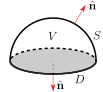
\includegraphics{OE08D_10.pdf}}}
\end{equation*}
Then the boundary, $\partial V$, of $V$ consists of two parts, namely $S$
(with normal pointing upwards) and the disk
\begin{equation*}
D=\Set{(x,y,0)}{x^2+y^2\le 1}
\end{equation*}
(with normal pointing downwards).  The divergence theorem (Theorem \eref{CLP317}{thm:divThm} of the CLP-4 text) 
gives
\begin{align*}
\dblInt_S \vF \cdot \hn\,\dee{S}
&=\tripInt_V \vnabla\cdot\vF\,\dee{V}
    -\dblInt_D \vF \cdot (-\hk)\,\dee{S} \\
&=\dblInt_D (x^2+y^2)\,\dee{x}\dee{y} 
\end{align*}
Switching to polar coordinates, the flux is
\begin{align*}
\dblInt_S \vF\cdot\hn\,\dee{S}
=\int_0^1\dee{r}\,r\int_0^{2\pi}\dee{\theta}\ r^2
=2\pi \int_0^1 \dee{r}\, r^3
=2\pi \tfrac{1}{4}
=\tfrac{\pi}{2}
\end{align*}

\end{solution}

%%%%%%%%%%%%%%%%%%%%%%%%%%%
\begin{question}[M317 2008A] %9

Let $S$ be the part of the paraboloid $z = 2 - x^2 - y^2$ contained 
in the cone $z = \sqrt{x^2+y^2}$ and oriented in the upward direction. 
Let
\begin{equation*}
\vF = (\tan \sqrt{z} + \sin(y^3))\,\hi + e^{-x^2}\,\hj + z\hk
\end{equation*}
Evaluate the flux integral $\dblInt_S \vF \cdot\hn\,\dee{S}$.
\end{question}

\begin{hint} 
As $\vF$ looks complicated, it is probably wise not to try and evaluate
the flux integral directly.
\end{hint}

\begin{answer} 
$\frac{3}{2}\pi$
\end{answer}

\begin{solution} 
As $\vF$ looks complicated, we will probably want to avoid evaluating
the flux integral directly. Let's first compute the divergence of $\vF$,
to see if it looks wise to use the divergence theorem instead.
\begin{align*}
\vnabla\cdot\vF = 
   \pdiff{}{x}\big(\tan \sqrt{z} + \sin(y^3)\big)
   +\pdiff{}{y}\big(e^{-x^2}\big)
   +\pdiff{}{z}\big(z\big)
=1
\end{align*}
Looks good! We cannot yet apply the divergence theorem, since $S$ is
not the boundary of a solid region $V$. To help us choose a solid 
$V$ whose boundary at least includes $S$, here is a sketch. $S$ is the
top of the ``ice cream cone''

\begin{center}
       \includegraphics{iceCream.pdf}
\end{center}
Note that the paraboloid $z = 2 - x^2 - y^2$ and the cone
$z = \sqrt{x^2+y^2}$ intersect along the circle $x^2+y^2=1$, $z=1$.
Probably the simplest solid whose boundary includes $S$ is
\begin{equation*}
V=\Set{(x,y,z)}{1\le z\le 2-x^2-y^2,\ x^2+y^2\le 1}
\end{equation*}
The boundary $\partial V$ of $V$ consists of $S$ (with upward pointing normal)
and the disk
\begin{equation*}
D = \Set{(x,y,z)}{x^2+y^2\le 1,\ z=1}
\end{equation*}
with normal $-\hk$. So the divergence theorem gives
\begin{align*}
\dblInt_S \vF \cdot\hn\,\dee{S}
&=\tripInt_V \vnabla\cdot\vF\ \dee{V} 
      -\dblInt_D \vF \cdot(-\hk)\,\dee{S} \\
&=\tripInt_V  \overbrace{1}^{\vnabla\cdot\vF}\dee{V} 
      +\dblInt_D \overbrace{1}^{\vF \cdot \hk = z}\,\dee{S} 
\end{align*}
As $D$ is a disk of radius 1, $\dblInt_D \dee{S}=\pi$. To compute the volume of
$V$, we'll slice it into a stack of horizontal ``pancakes''. Since
$z=2-x^2-y^2$ is equivalent to $\sqrt{x^2+y^2}=\sqrt{2-z}$, the pancake at height $z$
is a circular disk of radius $\sqrt{2-z}$ and hence of cross-sectional area
$\pi(2-z)$. So the volume of $V$ is
\begin{align*}
\tripInt_V  \dee{V}
&=\int_1^2 \pi(2-z) \ \dee{z}
= -\frac{\pi}{2}(2-z)^2\Big|_1^2
=\frac{\pi}{2}
\end{align*}
and the flux
\begin{align*}
\dblInt_S \vF \cdot\hn\,\dee{S}
=\frac{\pi}{2} +\pi =\frac{3}{2}\pi
\end{align*}

\end{solution}

%%%%%%%%%%%%%%%%%%%%%%%%%%%
\begin{question}[M317 2007A] %4
Evaluate the surface integral
\begin{equation*}
\dblInt_S \vF\cdot\hn\,\dee{S}
\end{equation*}
where $\vF(x, y, z) = \big(\cos z + xy^2\,,\, xe^{-z}\,,\, \sin y + x^2 z\big)$ 
and $S$ is the boundary of the solid region
enclosed by the paraboloid $z = x^2 + y^2$ and the plane $z = 4$, with outward pointing normal.
\end{question}

\begin{hint} 
As $\vF$ looks complicated, it is probably wise not to try and evaluate
the flux integral directly.
\end{hint}

\begin{answer} 
$\frac{32}{3}\pi$
\end{answer}

\begin{solution} 
As $\vF$ looks complicated, we will probably want to avoid evaluating
the flux integral directly. Let's first compute the divergence of $\vF$,
to see if it looks wise to use the divergence theorem instead.
\begin{align*}
\vnabla\cdot\vF = 
   \pdiff{}{x}\big(\cos z + xy^2\big)
   +\pdiff{}{y}\big(xe^{-z}\big)
   +\pdiff{}{z}\big(\sin y + x^2 z\big)
=y^2+x^2
\end{align*}
Looks promising. Furthermore $S$ is the boundary of the solid region
\begin{equation*}
V=\Set{(x,y,z)}{x^2+y^2\le z\le 4}
\hskip1.0in
\raisebox{-45pt}[65pt][30pt]{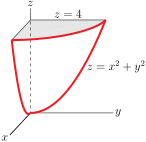
\includegraphics[scale=0.8]{OE07A_4.pdf}}
\end{equation*}
So the divergence theorem gives
\begin{align*}
\dblInt_S \vF \cdot\hn\,\dee{S}
&=\tripInt_V \vnabla\cdot\vF\ \dee{V} 
=\tripInt_V  (x^2+y^2)\ \dee{V} 
\end{align*}
To compute the triple integral, we'll use the cylindrical coordinates $(r,\theta,z)$.
The $z$-coordinate runs from $0$ to $4$. For each fixed $0\le z \le 4$
(see the blue disk in the figure below --- which shows the part of $V$ in the first octant),
\vadjust{
     \begin{center}
          \includegraphics{OE07A_4b.pdf}
     \end{center}
} 
$(x,y)$ runs over $0\le x^2+y^2 \le z$, which in cylindrical coordinates
is $0\le r^2\le z$ or $0\le r\le\sqrt{z}$. 
So the flux and the triple integral are
\begin{align*}
\dblInt_S \vF \cdot\hn\,\dee{S}
&=\tripInt_V  (x^2+y^2)\ \dee{V} \\
&=\int_0^4\dee{z}\int_0^{\sqrt{z}}\dee{r}\ r\int_0^{2\pi}\dee{\theta}\   r^2 \\
&=2\pi \int_0^4\dee{z}\int_0^{\sqrt{z}}\dee{r}\ r^3 \\
&=2\pi \int_0^4\dee{z}\ \frac{z^2}{4}
=2\pi \frac{4^3}{3\times 4}\\
&=\frac{32}{3}\pi
\end{align*}


\end{solution}

%%%%%%%%%%%%%%%%%%%%%%%%%%%%
\begin{question}[M317 2006D] %4
Let $S$ be the part of the sphere $x^2 + y^2 + z^2 = 4$ between the 
planes $z = 1$ and $z = 0$ oriented away from the origin. Let
\begin{align*}
\vF = (e^y + xz)\,\hi + (zy + \sin(x))\,\hj + (z^2 - 1)\,\hk
\end{align*}
Compute the flux integral
\begin{align*}
\dblInt_S \vF\cdot\hn\,\dee{S}.
\end{align*}
\end{question}

\begin{hint} 
The vector field $\vF$ looks complicated. Try to avoid a direct
evaluation of the flux integral.
\end{hint}

\begin{answer} 
$3\pi$
\end{answer}

\begin{solution}
If we were to evaluate this integral directly using, for example,
spherical coordinates, our integrand would contain
\begin{equation*}
\sin(x) = \sin\big(2\sin\varphi\cos\theta\big)
\end{equation*}
That's not very friendly looking. So let's consider using the divergence
theorem instead. To start, 
\begin{align*}
\vnabla\cdot\vF &= 
    \pdiff{}{x}\big(e^y + xz\big)
     +\pdiff{}{y}\big(zy + \sin(x)\big)
     +\pdiff{}{z}\big(z^2 - 1\big) 
   = 4z
\end{align*}
That's nice and simple. So let's move on to consideration of $S$.
The part of $S$ in the first octant is outlined in red in the figure 
on the left below.

\begin{center}
       \includegraphics{OE06D_4.pdf}\qquad
       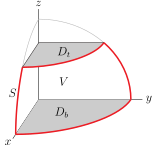
\includegraphics{OE06D_4b.pdf}
\end{center}

The surface $S$ is not closed, and so is not the boundary of a solid,
so we cannot apply the divergence theorem directly. But we can easily
come up with a solid whose boundary contains $S$. Let
\begin{equation*}
V=\Set{(x,y,z)}{ x^2 + y^2 + z^2 \le 4,\ 0\le z\le 1}
\end{equation*}
The boundary $\partial V$ of $V$ consists of three parts --- $S$,
the bottom disk
\begin{equation*}
D_b = \Set{(x,y,z)}{x^2 + y^2 \le 4,\ z=0}
\end{equation*}
and the top disk
\begin{equation*}
D_t = \Set{(x,y,z)}{x^2 + y^2 \le 3,\ z=1}
\end{equation*}
The outward normal to $D_t$ is $\hk$ and the outward normal to $D_b$ is $-\hk$.
So the divergence theorem gives
\begin{align*}
\tripInt_V\vnabla\cdot\vF\,\dee{V}
=\dblInt_{\partial V} \vF\cdot\hn\,\dee{S}
=\dblInt_S \vF\cdot\hn\,\dee{S}
  +\dblInt_{D_t} \vF\cdot\hk\,\dee{S}
  +\dblInt_{D_b} \vF\cdot(-\hk)\,\dee{S}
\end{align*}
On $D_b$, $z=0$ so that $\vF\cdot(-\hk) = -(0^2-1)=1$ and
on $D_t$, $z=1$ so that $\vF\cdot\hk = 1^2-1=0$.
So
\begin{align*}
\dblInt_S \vF\cdot\hn\,\dee{S}
=\tripInt_V\overbrace{4z}^{\vnabla\cdot\vF}\,\dee{V}
   -\dblInt_{D_b} \dee{S}
\end{align*}
The constant $z$ cross-section of $V$ is a disk of radius $\sqrt{4-z^2}$
and hence of area $\pi(4-z^2)$ and $D_b$ is a disk of radius $2$ and hence
of area $4\pi$. So
\begin{align*}
\dblInt_S \vF\cdot\hn\,\dee{S}
&=\int_0^1 (4z)\ \pi(4-z^2) \ \dee{z}  -4\pi 
=4\pi\Big[2z^2 - \frac{z^4}{4}\Big]_0^1 -4\pi
=3\pi
\end{align*}
\end{solution}


%%%%%%%%%%%%%%%%%%%%%%%%%%%
\begin{question}[M317 2006A] %7
Let $B$ be the solid region lying between the planes $x=-1$,
$x=1$, $y=0$, $y=2$ and bounded below by the plane $z=0$ and above 
by the plane $z+y=3$. Let $S$ be the surface of $B$. Find the flux 
of the vector field
\begin{equation*}
\vF(x,y,z) =  \big(x^2 z +\cos \pi y\big)\,\hi
             +\big(yz +\sin \pi z\big)\,\hj
             +(x-y^2)\,\hk
\end{equation*}
\end{question}

\begin{hint} 
The divergence of $\vF$ is a lot simpler than $\vF$ itself.
By default, we want the outward flux.
\end{hint}

\begin{answer} 
$\frac{26}{3}$
\end{answer}

\begin{solution}
The divergence of $\vF$, namely,
\begin{align*}
\vnabla\cdot\vF &= 
    \pdiff{}{x}\big(x^2 z +\cos \pi y\big)
     +\pdiff{}{y}\big(yz +\sin \pi z\big)
     +\pdiff{}{z}\big(x-y^2\big) \\
  &=2xz +z
\end{align*}
is a lot simpler than $\vF$ itself. So let's use the divergence theorem
(Theorem \eref{CLP317}{thm:divThm} of the CLP-4 text). 
\begin{align*}
\dblInt_S \vF \cdot \hn\,\dee{S}
=\tripInt_B \vnabla\cdot\vF\,\dee{V}
=\tripInt_B (2xz+z)\,\dee{V}
\end{align*}
As $B$ is invariant under $x\rightarrow-x$ while $2xz$ is odd under 
$x\rightarrow-x$, the integral $\tripInt_B 2xz\,\dee{V}$ is zero.
To help set up the limits of integration for $\tripInt_B z\,\dee{V}$,
note that, in $B$,
\begin{itemize}\itemsep1pt \parskip0pt \parsep0pt %\itemindent-15pt
\item[$\circ$]
$(x,y)$ runs over the rectangle $-1\le x\le 1$, $0\le y\le 2$ and
\item[$\circ$]
for each fixed $(x,y)$, $z$ runs over $0\le z\le 3-y$.
\end{itemize}
So
\begin{align*}
\dblInt_S \vF \cdot \hn\,\dee{S}
&= \int_{-1}^1\dee{x}\int_0^2\dee{y}\int_0^{3-y}\dee{z}\ z \\
&= \frac{1}{2}\int_{-1}^1\dee{x}\int_0^2\dee{y}\ (3-y)^2 \\
&=-\frac{1}{2}\int_{-1}^1\dee{x}\int_3^1\dee{u}\ u^2 \qquad
\text{with } u = 3-y,\ \dee{u}=-\dee{y} \\
&=-\frac{1}{2}\int_{-1}^1\dee{x}\ 
       \Big[\frac{1^3}{3} - \frac{3^3}{3}\Big]_{-1}^1\\
&=\frac{26}{3}
\end{align*}

\end{solution}

%%%%%%%%%%%%%%%%%%%%%%%%%%%
\begin{question}[M317 2005D] %9
Let $S$ be the hemisphere $x^2 + y^2 + z^2 = 1$, $z\ge 0$, 
oriented with $\hn$ pointing away from the origin. Evaluate the 
flux integral
\begin{equation*}
\dblInt_S \vF\cdot\hn\, \dee{S}
\end{equation*}
where
\begin{equation*}
\vF = \big(x + \cos(z^2)\big)\,\hi + \big(y + \ln(x^2 + z^5)\big)\,\hj 
           + \sqrt{x^2 + y^2}\,\hk
\end{equation*}
\end{question}

\begin{hint} 
The vector field $\vF$ looks very complicated. 
That strongly suggests that we not evaluate the integral directly.
\end{hint}

\begin{answer} 
$2\pi$
\end{answer}

\begin{solution}
The vector field $\vF$ looks very complicated. 
That strongly suggests that we not evaluate the integral directly.
So let's start by computing
\begin{align*}
\vnabla\cdot\vF &= 
    \pdiff{}{x}\big(x + \cos(z^2)\big)
     +\pdiff{}{y}\left(y + \ln(x^2 + z^5)\right)
     +\pdiff{}{z}\big(\sqrt{x^2 + y^2}\big) \\
   &=   2
\end{align*}
That's really simple, which suggest that we use the divergence theorem.
But the surface $S$ is not closed, and so is not the boundary of a solid.
So we cannot apply the divergence theorem directly. But we can easily
come up with a solid whose boundary contains $S$. Let
\begin{equation*}
V=\Set{(x,y,z)}{0\le z\le \sqrt{1-x^2-y^2},\ x^2+y^2\le 1}
    \hskip0.5in\raisebox{-40pt}[40pt][30pt]
                         {\includegraphics{OE05D_9.pdf}}
\end{equation*}
Then the boundary, $\partial V$, of $V$ consists of two parts, namely $S$
(with normal pointing upwards) and the disk
\begin{equation*}
D=\Set{(x,y,0)}{x^2+y^2\le 1}
\end{equation*}
(with normal $-\hk$).  The divergence theorem 
(Theorem \eref{CLP317}{thm:divThm} of the CLP-4 text) gives
\begin{align*}
\dblInt_S \vF \cdot \hn\,\dee{S}
&=\tripInt_V \vnabla\cdot\vF\,\dee{V}
    -\dblInt_D \vF \cdot (-\hk)\,\dee{S} \\
&=\tripInt_V 2\,\dee{V}
  +\dblInt_D \sqrt{x^2+y^2}\,\dee{x}\dee{y} 
&=2\ \frac{1}{2}\ \frac{4}{3}\pi 1^3
  +\dblInt_D \sqrt{x^2+y^2}\,\dee{x}\dee{y} 
\end{align*}
Switching to polar coordinates, the flux is
\begin{align*}
\dblInt_S \vF\cdot\hn\,\dee{S}
=\frac{4}{3}\pi+\int_0^1\dee{r}\,r\int_0^{2\pi}\dee{\theta}\ r
=\frac{4}{3}\pi + 2\pi \int_0^1 \dee{r}\, r^2
=\frac{4}{3}\pi + 2\pi \frac{1}{3}
=2\pi
\end{align*}

\end{solution}

%%%%%%%%%%%%%%%%%%%%%%%%%%%%%%%%%%%%%%%%%%%%
\begin{question}\label{prb_flux_surface}
Let $E$ be the solid region between the plane $z = 4$ and the paraboloid 
$z = x^2 + y^2$. Let
\begin{equation*}
\vF = \Big(-\frac{1}{3}x^3 + e^{z^2}\Big)\hi 
     + \Big(-\frac{1}{3}y^3 + x\sin z\Big)\hj + 4z\hk
\end{equation*}
\begin{enumerate}[(a)]
\item
Compute the flux of $\vF$ outward through the boundary of $E$.

\item
Let $S$ be the part of the paraboloid $z = x^2 + y^2$ lying below the 
$z = 4$ plane oriented with a normal vector $\hN$ that has a positive $\hk$ component. 
Compute the flux of $\vF$ through $S$.
\end{enumerate}

\end{question}

\begin{hint} 
The divergence of $\vF$ is a lot simpler than $\vF$ itself.
\end{hint}

\begin{answer} 
(a) $\frac{64}{3}\pi$\qquad
(b) $\frac{128}{3}\pi$
\end{answer}

\begin{solution} (a)
By the divergence theorem (Theorem \eref{CLP317}{thm:divThm} of the 
CLP-4 text), the outward flux of $\vF$ through the boundary of $E$ is
\begin{align*}
\dblInt_{\partial E}\vF\cdot\hn\,\dee{S}
&=\tripInt_E \vnabla\cdot\vF\,\dee{V} \\
&=\tripInt_E \big(-x^2-y^2+4\big)\,\dee{V} 
\end{align*}
To evaluate this integral we switch to cylindrical coordinates.
In cylindrical coordinates
\begin{equation*}
E=\Set{(r\cos\theta\,,\,r\sin\theta\,,\,z)}{0\le z\le 4,\ r^2\le z}
\end{equation*}
So
\begin{align*}
\dblInt_{\partial E}\vF\cdot\hn\,\dee{S}
&=\int_0^4\dee{z}\int_0^{\sqrt{z}}\dee{r}\,r\int_0^{2\pi}\dee{\theta}\ 
         \big(-r^2+4\big) \\
&=2\pi \int_0^4\dee{z}\int_0^{\sqrt{z}}\dee{r}\ \big(4r-r^3\big) \\
&=2\pi \int_0^4\dee{z}\ \Big(2z-\frac{z^2}{4}\Big) \\
&= 2\pi\Big[z^2-\frac{z^3}{12}\Big]_0^4
=2\pi\Big[16-\frac{16}{3}\Big]
=\frac{64}{3}\pi
\end{align*}

(b) The boundary of $E$ consists of two parts --- $S$, but with downward
pointing normal $\hn = -\hN$, on the bottom and the disk
\begin{equation*}
D =\Set{(x,y,z)}{z=4,\ x^2+y^2\le 4}
\end{equation*} 
with normal $\hk$, on top.
 \begin{center}
    \includegraphics{OE15A_6.pdf}
\end{center}
So, by part (a),
\begin{align*}
\frac{64}{3}\pi =\dblInt_{\partial E}\vF\cdot\hn\,\dee{S}
=-\dblInt_S \vF\cdot\hN\,\dee{S} 
  +\dblInt_D \vF\cdot\hk\,\dee{S}
=-\dblInt_S \vF\cdot\hN\,\dee{S} 
  +\dblInt_D \overbrace{4z}^{\vF\cdot\hk}\,\dee{S}
\end{align*}
Since $z=4$ on $D$, and $D$ is a disk of radius 2,
\begin{align*}
\dblInt_S \vF\cdot\hN\,\dee{S} 
=-\frac{64}{3}\pi +16\dblInt_D \dee{S}
=-\frac{64}{3}\pi +16(4\pi)
=\frac{128}{3}\pi
\end{align*}
\end{solution}

%%%%%%%%%%%%%%%%%%%%%%%%%%%%%%%
\begin{question}[M317 2012J] %8
Consider the vector field
\begin{equation*}
\vF(x,y,z) = \frac{x\,\hi+y\,\hj+z\,\hk}
                  {{[x^2 + y^2 + z^2\big]}^{3/2}}
\end{equation*}
\begin{enumerate}[(a)]
\item
   Compute $\vnabla\cdot\vF$.
\item
Let $S_1$ be the sphere given by
\begin{equation*}
x^2 + (y - 2)^2 + z^2 = 9
\end{equation*}
oriented outwards. Compute
$\dst\dblInt_{S_1} \vF\cdot\hn\,\dee{S}$.
\item
Let $S_2$ be the sphere given by
\begin{equation*}
x^2 + (y - 2)^2 + z^2 = 1
\end{equation*}
oriented outwards. Compute
$\dst\dblInt_{S_2} \vF\cdot\hn\,\dee{S}$.
\item
Are your answers to (b) and (c) the same or different? Give a 
mathematical explanation of your answer.
\end{enumerate}

\end{question}

\begin{hint} 
Note that $\vF(x,y,z)$ is not defined at $(x,y,z)=(0,0,0)$.
\end{hint}

\begin{answer} 
(a) $\vnabla\cdot\vF=0$ if $(x,y,z)\ne\vZero$ and is not defined if $(x,y,z)=\vZero$.

(b) $4\pi$\qquad
(c) $0$

(d) The flux integrals $\dblInt_{S_1} \vF\cdot\hn\,\dee{S}$ and
$\dblInt_{S_2} \vF\cdot\hn\,\dee{S}$ are different, because the one point,
$(0,0,0)$, where $\vnabla\cdot\vF$ fails to be well-defined and zero,
is contained inside $S_1$ but is not contained inside $S_2$.
\end{answer}

\begin{solution} (a) Since
\begin{alignat*}{3}
\pdiff{}{x}\frac{x}{{[x^2+y^2+z^2]}^{3/2}}
&=\frac{1}{{[x^2+y^2+z^2]}^{3/2}} 
            -\frac{3}{2}\frac{x(2x)}{{[x^2+y^2+z^2]}^{5/2}}
&\,=\,\frac{-2x^2+y^2+z^2}{{[x^2+y^2+z^2]}^{5/2}}
\\
\pdiff{}{y}\frac{y}{{[x^2+y^2+z^2]}^{3/2}}
&=\frac{1}{{[x^2+y^2+z^2]}^{3/2}} 
            -\frac{3}{2}\frac{y(2y)}{{[x^2+y^2+z^2]}^{5/2}}
&\,=\,\frac{x^2-2y^2+z^2}{{[x^2+y^2+z^2]}^{5/2}}
\\
\pdiff{}{z}\frac{z}{{[x^2+y^2+z^2]}^{3/2}}
&=\frac{1}{{[x^2+y^2+z^2]}^{3/2}} 
            -\frac{3}{2}\frac{z(2z)}{{[x^2+y^2+z^2]}^{5/2}}
&\,=\,\frac{x^2+y^2-2z^2}{{[x^2+y^2+z^2]}^{5/2}}
\end{alignat*}
the specified divergence is
\begin{align*}
\vnabla\cdot\vF 
           &=  \frac{(-2x^2+y^2+z^2) + (x^2-2y^2+z^2) + (x^2+y^2-2z^2)}
                     {{[x^2+y^2+z^2]}^{5/2}}
           =0
\end{align*}
if $(x,y,z)\ne\vZero$ and is not defined if $(x,y,z)=\vZero$.

(b), (c) Set
\begin{align*}
V_1 &= \Set{(x,y,z)}{x^2 + (y - 2)^2 + z^2 \le 9} \\
V_2 &= \Set{(x,y,z)}{x^2 + (y - 2)^2 + z^2 \le 1} 
\end{align*}
Here are side views of both $V_1$ and $V_2$.
\vadjust{
\begin{center}
     \includegraphics[scale=0.90]{OE12J_8a.pdf}\qquad\qquad
     \includegraphics[scale=0.90]{OE12J_8b.pdf}
\end{center}
}%
Both $V_1$ and $V_2$ are spherical balls centred on $(0,2,0)$.
The difference between them is that $V_1$ has radius $3$ while $V_2$
has radius $1$. In particular $(0,0,0)$ is not in $V_2$. So $\vnabla\cdot\vF$ is 
well-defined and zero throughout $V_2$ and, by the divergence theorem
(Theorem \eref{CLP317}{thm:divThm} of the CLP-4 text),
\begin{align*}
\dblInt_{S_2} \vF\cdot\hn\,\dee{S}
=\tripInt_{V_2} \vnabla\cdot\vF\,\dee{V}
=0
\end{align*}
On the other hand, $(0,0,0)$ is in $V_1$. We cannot blindly apply the divergence
theorem to $V_1$ --- $\vnabla\cdot\vF(x,y,z)$ is not defined at the point
$(x,y,z)=(0,0,0)$ in $V_1$. We can work around this obstruction
by 
\begin{itemize}\itemsep1pt \parskip0pt \parsep0pt %\itemindent-15pt
\item[$\circ$]
choosing a number $\rho>0$ that is small enough that the sphere
\begin{equation*}
S_\rho = \Set{(x,y,z)}{x^2+y^2+z^2=\rho^2}
\end{equation*}
is completely contained inside $V_1$ (for example, $\rho=\frac{1}{2}$ is fine)
\item[$\circ$]
and then removing the interior of $S_\rho$ from $V_1$. 
\end{itemize}
This produces
\begin{equation*}
V_3 = \Set{(x,y)}{x^2 + (y - 2)^2 + z^2 \le 9,\ x^2+y^2+z^2\ge\rho^2}
\end{equation*}
whose side view is sketched below.
 \begin{center}
    \includegraphics{OE12J_8c.pdf}
\end{center}
The boundary of $V_3$ consists of two parts
\begin{itemize}\itemsep1pt \parskip0pt \parsep0pt %\itemindent-15pt
\item[$\circ$]
the sphere $S_1$, with outward normal and
\item[$\circ$]
the sphere $S_\rho$ with \emph{inward} normal $\hn=-\frac{\vr}{|\vr|}$
\end{itemize}
The divergence $\vnabla\cdot\vF$ is well-defined and zero throughout $V_3$ 
so that, by the divergence theorem,
\begin{align*}
0=\tripInt_{V_3} \vnabla\cdot\vF\,\dee{V}
=\dblInt_{S_1} \vF\cdot\hn\,\dee{S} 
 +\dblInt_{S_\rho} \vF\cdot\Big(-\frac{\vr}{|\vr|}\Big)\,\dee{S}
\end{align*}
So
\begin{align*}
\dblInt_{S_1} \vF\cdot\hn\,\dee{S}
&=\dblInt_{S_\rho} \vF\cdot\Big(\frac{\vr}{|\vr|}\Big)\,\dee{S}
=\dblInt_{S_\rho} \Big(\frac{\vr}{|\vr|^3}\Big)\cdot\Big(\frac{\vr}{|\vr|}\Big)\,\dee{S}
=\dblInt_{S_\rho} \frac{1}{|\vr|^2}\,\dee{S}
=\dblInt_{S_\rho} \frac{1}{\rho^2}\,\dee{S} \\
&=\frac{1}{\rho^2}\ 4\pi\rho^2=4\pi
\end{align*}
since $S_\rho$ is a sphere of radius $\rho$ and hence of surface area $4\pi\rho^2$.

(d) The flux integrals $\dblInt_{S_1} \vF\cdot\hn\,\dee{S}$ and
$\dblInt_{S_2} \vF\cdot\hn\,\dee{S}$ are different, because the one point,
$(0,0,0)$, where $\vnabla\cdot\vF$ fails to be well-defined and zero,
is contained inside $S_1$ but is not contained inside $S_2$.
\end{solution}

%%%%%%%%%%%%%%%%%%%%%%%%%%%%%%%
\begin{question}[M317 2016D] %8
Let $\vF$ be the vector field defined by
\begin{equation*}
\vF(x,y, z) = \big(y^3 z + 2x\big)\,\hi 
             +\big(3y - e^{\sin z}\big)\,\hj + \big(e^{x^2+y^2}+ z\big)\,\hk
\end{equation*}
Calculate the flux integral $\dblInt_S \vF\cdot\hn\,\dee{S}$
where $S$ is the boundary surface of the solid region
\begin{equation*}
E\ :\ 
0 \le x \le 2,\quad
0 \le y \le 2,\quad
0 \le z \le 2+ y
\end{equation*}
with outer normal.
\end{question}

%\begin{hint} 
%
%\end{hint}

\begin{answer} 
$72$
\end{answer}

\begin{solution} 
The vector field $\vF$ looks pretty complicated. But its divergence
\begin{equation*}
\vnabla\cdot\vF = 2 + 3 + 1 = 6
\end{equation*}
is very simple. So let's use the divergence theorem
(Theorem \eref{CLP317}{thm:divVrn} of the CLP-4 text). It says
\begin{align*}
\dblInt_S \vF\cdot\hn\,\dee{S}
&=\tripInt_E \vnabla\cdot\vF\ \dee{V}
=\tripInt_E 6\ \dee{V}
=6\ \text{Volume}(E)
\end{align*}
For any fixed $0\le X\le 2$, the cross-section of $E$ with $x=X$ has side view
\begin{center}
     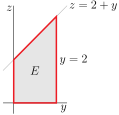
\includegraphics{OE16D_8.pdf}
\end{center}
That cross-section has area $2\times \frac{2+4}{2}=6$. Consequently the 
volume of $E$ is $2\times 6=12$ and
\begin{equation*}
\dblInt_S \vF\cdot\hn\,\dee{S}
=6\times 12
=72
\end{equation*}
\end{solution}

%%%%%%%%%%%%%%%%%%%%%%%%%%%
\begin{question}[M317 2017A] %7
Consider the vector field
\begin{equation*}
 \vF(x, y, z) = \big(z \arctan(y^2)\,,\, z^3 \ln(x^2 + 1)\,,\, 3z\big)
\end{equation*}
Let the surface $S$ be the part of the sphere $x^2 + y^2 + z^2 = 4$ 
that lies above the plane $z = 1$ and be oriented downwards.
\begin{enumerate}[(a)]
\item
Find the divergence of $\vF$.

\item
Compute the flux integral $\dblInt_S \vF \cdot\hn\,\dee{S}$.

\end{enumerate}
\end{question}

\begin{hint} 
The surface S is not a closed surface.
\end{hint}

\begin{answer} 
(a) $3$\qquad
(b) $-14\pi$
\end{answer}

\begin{solution} (a) The divergence is
\begin{align*}
\vnabla\cdot\vF
&=\pdiff{}{x}\big(z \arctan(y^2)\big)
      +  \pdiff{}{y}\big(z^3 \ln(x^2 + 1)\big)
      +  \pdiff{}{z}\big(3z\big) 
= 3
\end{align*}

(b) The complexity of $\vF$ and the simplicity of $\vnabla\cdot\vF$
strongly suggest that we use the divergence theorem to evaluate
$\dblInt_S \vF \cdot\hn\,\dee{S}$. However, $S$ is \emph{not} a closed
surface and is \emph{not} the boundary of a solid. The figure on the left below
is a sketch of the part of $S$ in the first octant.
\begin{center}
     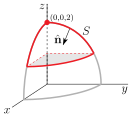
\includegraphics{OE17A_7a}\qquad
     \includegraphics{OE17A_7b}
\end{center}
On the other hand $S$ is part of the surface of the solid
\begin{equation*}
V=\Set{(x,y,z)}{x^2+y^2+z^2\le 4,\ z\ge 1}
\end{equation*}
which is sketched on the right above. The boundary of $V$ consists of two parts:
\begin{itemize}\itemsep1pt \parskip0pt \parsep0pt %\itemindent-15pt
\item[$\circ$]
the original surface $S$, but with upward, rather than downward, normal and
\item[$\circ$]
the disk $D=\Set{(x,y,z)}{ x^2+y^2\le 3,\ z=1}$ with normal $-\hk$.
\end{itemize}
So the divergence theorem (Theorem \eref{CLP317}{thm:divVrn} in the 
CLP-4 text) gives
\begin{align*}
   \dblInt_{\partial V}\vF\cdot\hn\,\dee{S} 
           &= \tripInt_V\vnabla\cdot\vF\ \dee{V}
           = 3 \tripInt_V \dee{V} \\
\implies
  -\dblInt_S\vF\cdot\hn\,\dee{S} +\dblInt_D\vF\cdot(-\hk)\,\dee{S} 
           &=3\,\text{Volume}(V)
\end{align*}
Thus
\begin{align*}
\dblInt_S\vF\cdot\hn\,\dee{S} &= -3\,\text{Volume}(V)
                      + \dblInt_D\overbrace{-3}^{-\vF\cdot\hk}\,\dee{S} \\
&= -3\,\text{Volume}(V) -3\,\text{Area}(D) \\
&= -3\,\text{Volume}(V) -9\pi
\end{align*}
since $D$ is a circular disk of radius $\sqrt{3}$. To compute the volume
of $V$, we slice $V$ into thin horizontal pancakes each of thinkness $\dee{z}$. 
The pancake at height $z$ has cross-section the circular disk 
$x^2+y^2\le 4-z^2$. As this disk has area $\pi(4-z^2)$, the pancake has volume 
$\pi(4-z^2)\,\dee{z}$. All together
\begin{align*}
\text{Volume}(V)
&=\int_1^2\dee{z}\ \pi(4-z^2)
=\pi\left[4z-\frac{z^3}{3}\right]_1^2
=\pi\left[4-\frac{7}{3}\right]
=\frac{5\pi}{3}
\end{align*}
and
\begin{equation*}
\dblInt_S\vF\cdot\hn\,\dee{S} =-3\frac{5\pi}{3}-9\pi
=-14\pi
\end{equation*}
\end{solution}

%%%%%%%%%%%%%%%%%%%%%%%%%%%%%%%
\begin{question}[M317 2017D] %9
Let $S$ be the sphere $x^2+y^2+z^2=3$ oriented inward. 
Compute the flux integral
\begin{equation*}
\dblInt_S\vF\cdot\hn\,\dee{S}
\end{equation*}
where
\begin{equation*}
\vF = \big(xy^2 + y^4z^6\,,\, yz^2+x^4z\,,\,zx^2+xy^4\big)
\end{equation*}
\end{question}

%\begin{hint} 
%\end{hint}

\begin{answer} 
$-\frac{4\,\pi}{5}\ 3^{5/2}$
\end{answer}

\begin{solution} 
Let's try the divergence theorem. Set
\begin{equation*}
V = \Set{(x,y,z)}{x^2+y^2+z^2\le 3}
\end{equation*}
Then the boundary of $V$ is $S$, but with outward pointing normal. 
Since
\begin{equation*}
\vnabla\cdot\vF = 
   \pdiff{}{x} \big(xy^2 + y^4z^6\big)
 + \pdiff{}{y} \big(yz^2+x^4z\big) 
 + \pdiff{}{z} \big(zx^2+xy^4\big)
=y^2+z^2+x^2
\end{equation*}
and because $S$ is oriented \emph{inward}, the divergence theorem 
(Theorem \eref{CLP317}{thm:divThm} of the CLP-4 text)
gives
\begin{align*}
\dblInt_S\vF\cdot\hn\,\dee{S}
         &=-\tripInt_V \vnabla\cdot\vF\,\dee{V}
          = -\tripInt_V (x^2+y^2+z^2)\,\dee{V}
\end{align*}
Switching to spherical coordinates (see Appendix \eref{CLP317}{ap:spherCoord}
in the CLP-4 text)
\begin{align*}
\dblInt_S\vF\cdot\hn\,\dee{S}
&=-\int_0^{\sqrt{3}}\dee{\rho}\int_0^\pi\dee{\varphi}
             \int_0^{2\pi}\dee{\theta} \ \rho^4\sin\varphi \\
&=-2\pi\left[\int_0^{\sqrt{3}}\dee{\rho}\ \rho^4\right]
      \left[\int_0^\pi\dee{\varphi}\ \sin\varphi\right] \\
&=-2\pi\left[\frac{\rho^5}{5}\right]_0^{\sqrt{3}}
      \Big[-\cos\varphi\Big]_0^\pi \\
&=-\frac{36\sqrt{3}}{5}\pi
\end{align*}
\end{solution}

%%%%%%%%%%%%%%%%%%%%%%%%%%%
\begin{question}[M317 2004A] %6
Consider the vector field $\vF(x,y,z)
=-2xy\,\hi+\big(y^2+\sin(xz)\big)\,\hj+(x^2+y^2)\,\hk$.
\begin{enumerate}[(a)]
\item 
Calculate $\nabla\cdot \vF$. 
\item
Find the flux of $\vF$ through the surface $S$ defined by
\begin{equation*}
x^2+y^2+(z-12)^2=13^2,\ z\ge 0
\end{equation*}
using the outward normal to $S$.
\end{enumerate}
\end{question}

%\begin{hint} 
%\end{hint}

\begin{answer} 
(a) $0$\qquad
(b) $\frac {625}{2}\pi$
\end{answer}

\begin{solution} 
(a) The divergence of $\vF$ is
\begin{equation*}
\nabla\cdot \vF
=\pdiff{}{x}\big(-2xy\big)
+\pdiff{}{y}\big(y^2+\sin(xz)\big)
+\pdiff{}{z}\big(x^2+y^2\big)
=-2y+2y+0=0
\end{equation*}

(b)
Call the specified surface $S$ and set
\begin{equation*}
V = \Set{(x,y,z)}{x^2+y^2+(z-12)^2\le 13^2,\ z\ge 0}
\end{equation*}
The boundary, $\partial V$, of $V$ consists of two parts ---
$S$, with outward normal, and the disk
\begin{equation*}
D = \Set{(x,y,z)}{x^2+y^2\le 13^2-12^2=5^2,\ z=0}
\end{equation*}
with normal $-\hk$.
By the divergence theorem, the desired flux is
\begin{align*}
\dblInt_S\vF\cdot\hn\ \dee{s}
&=\tripInt_V\nabla\cdot \vF\ \dee{V} - \dblInt_D \vF\cdot(-\hk)\ \dee{S}\\
&=\tripInt_V 0 \ \dee{V} + \dblInt_D (x^2+y^2) \dee{x}\dee{y} \\
&=0 +\int_0^5\dee{r}\ r\int_0^{2\pi}\dee{\theta}\ r^2 \\
&=2\pi\frac{5^4}{4} = \frac {625}{2}\pi
\end{align*}
\end{solution}

%%%%%%%%%%%%%%%%%%%%%%%%%%%
\begin{question}[M317 2003A] %6
Let $S$ be the portion of the hyperboloid $x^2 + y^2 -z^2 = 1$ 
between $z=-1$ and $z=1$. Find the flux of 
$\vF = (x+e^{yz})\,\hi +\big(2yz+\sin(xz)\big)\,\hj +(xy-z-z^2)\,\hk$ 
out of $S$ (away from the origin).
\end{question}

%\begin{hint} 
%\end{hint}

\begin{answer} 
$4\pi$
\end{answer}

\begin{solution} 
The boundary of the solid $V$ enclosed by $S$ and $z= \pm 1$ consists 
of three pieces: $S$, the top disk 
\begin{equation*}
S_1=\Set{(x,y,z)}{x^2 + y^2 \le 2,\ z= 1}
\end{equation*} 
and the bottom disk 
\begin{equation*}
S_2=\Set{(x,y,z)}{x^2 + y^2 \le 2,\ z= -1}
\end{equation*}
On $S_1$, $\hn=\hk$ and 
\begin{equation*}
\vF\cdot\hn=\vF\cdot\hk=xy-z-z^2\Big|_{z=1}= xy-2
\end{equation*} so that,
denoting $D=\Set{(x,y)}{x^2+y^2 \le 2}$,
$$
\dblInt_{S_1} \vF \cdot \hn\, \dee{S} 
   = \dblInt_D (xy -2) \,\dee{x}\dee{y} 
   =-2\,\text{Area}(D)= - 4 \pi
$$
Here we have used that the integral $\dblInt_D xy \,\dee{x}\dee{y}=0$
because $xy$ is odd under $x\rightarrow -x$.
On $S_2$, $\hn=-\hk$ and 
\begin{equation*}
\vF\cdot\hn=-\vF\cdot\hk= -(xy-z-z^2)\Big|_{z=-1}=-xy
\end{equation*} 
so that
$$
\dblInt_{S_2} \vF \cdot \hn\, \dee{S} = \dblInt_D (- xy)\,  \dee{x}\dee{y} = 0
$$
By the divergence theorem (Theorem \eref{CLP317}{thm:divThm} in 
the CLP-4 text),
\begin{align*}
\dblInt_S \vF \cdot \hn \dee{S} 
= \dblInt_V \vnabla\cdot\vF\, \dee{V} - 
 \dblInt_{S_1} \vF \cdot \hn\, \dee{S}
- \dblInt_{S_2} \vF \cdot \hn\, \dee{S} = 0 -(- 4 \pi) - 0 
= 4\pi
\end{align*}
since 
\begin{align*}
\vnabla\cdot\vF &= 
    \pdiff{}{x}(x+e^{yz})
     +\pdiff{}{y}\big(2yz+\sin(xz)\big)
     +\pdiff{}{z}(xy-z-z^2) \\
   &=   1 + 2z -1 -2z \\
   &=0
\end{align*}
\end{solution}

%%%%%%%%%%%%%%%%%%%%%%%%%%%
\begin{question}[M317 2002A] %7
Let $\vF$ be the vector field
$\vF(x,y,z)=(x^2-y-1)\,\hi+(e^{\cos y}+z^3)\,\hj+(2xz+z^5)\,\hk$.
Evaluate $\dblInt_S\vnabla\times \vF\cdot\hn\,\dee{S}$ where $S$ is the part
of the ellipsoid $x^2+y^2+2z^2=1$ with $z\ge 0$.
\end{question}

\begin{hint} 
The complexity of $\vF$ is a hint that the flux should
not be evaluated directly.
\end{hint}

\begin{answer} 
$\pi$
\end{answer}

\begin{solution} 
\emph{Direct Solution.}
The surface is given by the implicit equation
$f(x,y,z)=0$ with $f(x,y,z)=x^2+y^2+2z^2-1$. Hence,
 by (\eref{CLP317}{eq:SUdSimplicit}) in the CLP-4 text,
$$
\hn\,\dee{S}=\frac{\vnabla f}{\vnabla f\cdot\hk}\dee{x}\dee{y}
=\frac{2x\hi+2y\hj+4z\hk}{4z}\dee{x}\dee{y}
$$
This $\hn$ has positive $\hk$ component. Assume that it is the desired
$\hn$, though this was not specified in the question.
Since
\begin{align*}
\vnabla\times\vF
&=\det\left[\begin{matrix}
\hi &\hj &\hk \\
\tfrac{\partial\hfill}{\partial x} & \tfrac{\partial\hfill}{\partial y} & 
                \tfrac{\partial\hfill}{\partial z} \\
x^2-y-1 & e^{\cos y}+z^3 & 2xz+z^5
\end{matrix}
\right] \\
&=-3z^2\,\hi-2z\,\hj+\hk
\end{align*}
we have
\begin{align*}
\dblInt_S\vnabla\times \vF\cdot\hn\,\dee{S}
&=\dblInt_{x^2+y^2\le 1}\big(-3z(x,y)^2\,\hi-2z(x,y)\,\hj+\hk\big)
   \cdot\frac{2x\,\hi+2y\,\hj+4z(x,y)\,\hk}{4z(x,y)}\ \dee{x}\dee{y}
\\
&=\dblInt_{x^2+y^2\le 1}\Big(-\frac{3}{2}x\,z(x,y)-y+1\Big)\ \dee{x}\dee{y}
\end{align*}
Since $y$ is an odd function of $y$ and $x\,z(x,y)=x\sqrt{\half(1-x^2-y^2)}$
is an odd function of $x$, they both integrate to zero. Hence
$$
\dblInt_S\vnabla\times \vF\cdot\hn\,\dee{S}
=\dblInt_{x^2+y^2\le 1}1\ \dee{x}\dee{y}
=\pi
$$

\smallskip
\noindent\emph{Tricky Solution.}
 Let $V$ be the solid $x^2+y^2+2z^2\le 1$,
$z\ge 0$. The surface of $V$ consists of $S$ with upward pointing normal
and the disk $D=\Set{(x,y,z)}{z=0,\ x^2+y^2\le 1}$ with normal $-\hk$.
By the divergence theorem, Theorem \eref{CLP317}{thm:divThm} in the CLP-4
text,
$$
\dblInt_S\vnabla\times \vF\cdot\hn\,\dee{S}
+\dblInt_D\vnabla\times \vF\cdot(-\hk)\,\dee{S}
=\tripInt_V\vnabla\cdot\vnabla\times\vF\ \dee{V}
=\tripInt_V 0\ \dee{V}=0
$$
Hence
$$
\dblInt_S\vnabla\times \vF\cdot\hn\,\dee{S}
=\dblInt_D\vnabla\times \vF\cdot\hk\,\dee{S}
=\dblInt_D \dee{S}
=\pi
$$
\end{solution}


%%%%%%%%%%%%%%%%%%%%%%%%%%%
\begin{question}[M317 2001A] %4
Let $S$ be the portion of the sphere $x^2+y^2+(z-1)^2=4$
that lies above the $xy$-plane. Find the flux of 
$\vF=(x^2+e^{y^2})\,\hi+(e^{x^2}+y^2)\,\hj +(4+5x)\,\hk$ outward across
$S$.
\end{question}

%\begin{hint} 
%\end{hint}

\begin{answer} 
$12\pi$
\end{answer}

\begin{solution} 
Let $S'$ be the disk $x^2+y^2\le 3,\ z=0$ (with $\hn$ the downward 
pointing normal) and let $V$
be the portion of the ball $x^2+y^2+(z-1)^2\le 4$ with $z\ge 0$. 
Then, by the divergence theorem,
\begin{align*}
\dblInt_{S}\vF\cdot\hn\,\dee{S}
&=\tripInt_{V}\vnabla\cdot\vF\, \dee{V}
-\dblInt_{S'}\vF\cdot(-\hk)\,\dee{S}\\
&=\tripInt_{V}(2x+2y)\, \dee{V}
+\dblInt_{S'}(4+5x)\,\dee{x}\dee{y}
\end{align*}
Because $x$ is odd under $x\rightarrow-x$ and $y$ is odd under
$y\rightarrow -y$,
\begin{equation*}
\tripInt_{V}x\, \dee{V}=\tripInt_{V}y\, \dee{V}=\dblInt_{S'}x\,\dee{x}\dee{y}=0
\end{equation*}
so that
\begin{align*}
\dblInt_{S}\vF\cdot\hn\,\dee{S}
=4\dblInt_{S'}\,\dee{x}\dee{y}
=4\,\text{Area}(S')
=4\times \pi\big(\sqrt{3}\big)^2=12\pi 
\end{align*}

\end{solution}

%%%%%%%%%%%%%%%%%%%%%%%%%%%
\begin{question}[M317 1999A] %5
Find the flux of $\vF=xy^2\hi+x^2y\hj+\hk$ outward through
the hemispherical surface 
\begin{equation*}
x^2+y^2+z^2=4,\qquad z\ge 0
\end{equation*}
\end{question}

\begin{hint} 
The flux can be calculated directly, but it is rather easier to 
calculate it using the Divergence Theorem.
\end{hint}

\begin{answer} 
$\frac{188}{15}\pi\approx39.37$
\end{answer}

\begin{solution} 
Call the hemisphere $0\le z\le \sqrt{4-x^2-y^2}$, $H$.
Call the bottom surface of the hemisphere $D$ and the top surface $S$.
The disk $D$ has radius $2$, area $4\pi$, $z=0$ and 
the outward normal $-\hk$, so that
$$
\dblInt_{D}\vF\cdot\hn\,\dee{S}
=-\dblInt_{D}\vF\cdot\hk\,\dee{x}\dee{y}
=-\dblInt_D\,\dee{x}\dee{y}
=-4\pi
$$
As
$$
\vnabla\cdot\vF
=\pdiff{}{x}(xy^2)
+\pdiff{}{y}(x^2y)
+\pdiff{}{z}(1)
=x^2+y^2
$$
the divergence theorem (Theorem \eref{CLP317}{thm:divThm} of the CLP-4 text) 
gives
\begin{align*}
\dblInt_{\cS}\vF\cdot\hn\,\dee{S}
&=\tripInt_H\vnabla\cdot\vF\ \dee{V}
-\dblInt_D\vF\cdot\hn\,\dee{S}
=\tripInt_R(x^2+y^2)\ \dee{V}
-(-4\pi)
\end{align*}
To evaluate the remaining integral, let's switch to the
cylindrical coordinates $(r,\theta,z)$. In cylindrical coordinates,
the equation $x^2+y^2+z^2=4$ becomes $r^2+z^2=4$. So
\begin{align*}
\dblInt_{\cS}\vF\cdot\hn\,\dee{S}
&=4\pi+\int_0^2 \dee{z}\int_0^{\sqrt{4-z^2}}dr\ r\int_0^{2\pi}\dee{\theta}\ r^2
=4\pi+2\pi\int_0^2 \dee{z}\ \frac{1}{4}\big(\sqrt{4-z^2}\big)^4\\
&=4\pi+\frac{\pi}{2}\int_0^2 \dee{z}\ (16-8z^2+z^4\big)
=4\pi+\frac{\pi}{2}\Big[16z-\frac{8}{3}z^3+\frac{1}{5}z^5\Big]_0^2 \\
&=\frac{188}{15}\pi\approx39.37
\end{align*}
\end{solution}

%%%%%%%%%%%%%%%%%%%%%%%%%%%
\begin{question}[M317 1998D] %5
 Let $D$ be the cylinder $x^2+y^2\le 1$, $0\le z\le 5$. Calculate
the flux of the vector field
$$
\vF=(x+xye^z)\,\hi+\half y^2ze^z\,\hj+(3z-yze^z)\,\hk
$$
outward through the curved part of the surface of $D$.
\end{question}

\begin{hint} 
Use that $y$ is odd to easily evaluate some integrals.
\end{hint}

\begin{answer} 
$5\pi$
\end{answer}

\begin{solution} 
Let $S_t$, $S_b$ and $S_c$ denote the top, bottom and curved surfaces of
$D$ respectively. On the top surface, $z=5$ and 
the outward normal to $D$ is $\hk$, so that
$$
\dblInt_{\cS_t}\vF\cdot\hn\,\dee{S}
=\dblInt_{x^2+y^2\le 1}(15-5ye^5)\,\dee{x}\dee{y}
=15\dblInt_{x^2+y^2\le 1}\,\dee{x}\dee{y}
=15\pi
$$
The integral over $y$ was zero because $y$ is odd under $y\rightarrow -y$.
On the bottom surface, $z=0$ and 
the outward normal to $D$ is $-\hk$, so that
$$
\dblInt_{\cS_b}\vF\cdot\hn\,\dee{S}
=-\dblInt_{x^2+y^2\le 1}(3\times 0-0\times ye^0)\,\dee{x}\dee{y}
=0
$$
Again, the integral over $y$ was zero because $y$ is odd under 
$y\rightarrow -y$. As
$$
\vnabla\cdot\vF
=\pdiff{}{x}(x+xye^z)
+\half\pdiff{}{y}\big( y^2ze^z\big)
+\pdiff{}{z}(3z-yze^z)
=(1+ye^z)+yze^z+(3-yze^z-ye^z)
=4
$$
the divergence theorem gives
\begin{align*}
\dblInt_{\cS_c}\vF\cdot\hn\,\dee{S}
&=\tripInt_D\vnabla\cdot\vF\ \dee{V}
-\dblInt_{\cS_t}\vF\cdot\hn\,\dee{S}
-\dblInt_{\cS_b}\vF\cdot\hn\,\dee{S}\\
&=\tripInt_D4\ \dee{V}
-15\pi-0
=4\times\pi 1^2\times 5-15\pi
=5\pi
\end{align*}
\end{solution}

%%%%%%%%%%%%%%%%%%%%%%%%%%%%%%%%
\begin{question}
Find the flux of $\vF=(y+xz)\hi+(y+yz)\hj-(2x+z^2)\hk$ upward
through the first octant part of the sphere $x^2+y^2+z^2=a^2$.
\end{question}

%\begin{hint} 
%
%\end{hint}

\begin{answer} 
$\left[\frac{\pi}{6}-\frac{1}{3}\right]a^3$
\end{answer}

\begin{solution} 
Let $V=\Set{(x,y,z)}{x^2+y^2+z^2\le a^2, x\ge 0, y\ge 0,\ z\ge 0}$. 
\begin{center}
       \includegraphics{quartSph.pdf}
\end{center}
Then $\partial V$ consists of
\begin{itemize}\itemsep1pt \parskip0pt \parsep0pt %\itemindent-15pt
\item
   the $x=0$ face $\Set{(x,y,z)}{y^2+z^2\le a^2, x=0, y\ge 0,\ z\ge 0}$
   with normal $\hn=-\hi$, 
\item
   the $y=0$ face $\Set{(x,y,z)}{x^2+z^2\le a^2, x\ge 0, y= 0,\ z\ge 0}$
   with normal $\hn=-\hj$, 
\item
   the $z=0$ face $\Set{(x,y,z)}{x^2+y^2\le a^2, x\ge 0, y\ge 0,\ z= 0}$
   with normal $\hn=-\hk$, 
\item
   and the first octant part of the sphere. Call it $S$. 
\end{itemize}
Then
\begin{align*}
&\tripInt_V \vnabla\cdot\vF\,\dee{V}=\tripInt_V\big[z+1+z-2z\big]\,\dee{V}
=\tripInt_V \,\dee{V}=\frac{1}{8}\ \frac{4}{3}\pi a^3=\frac{1}{6}\pi a^3\\
%
&\dblInt_{\Atop{z=0}{\rm face}}\vF\cdot(-\hk)\,\dee{x}\,\dee{y}
=\dblInt_{\Atop{z=0}{\rm face}}(2x+0^2)\,\dee{x}\,\dee{y}
=2\int_0^a dr\,r\int_0^{\pi/2}\dee{\theta}\ r\cos\theta
=2\int _0^a r^2\,dr
=\frac{2a^3}{3}\\
%
&\dblInt_{\Atop{y=0}{\rm face}}\vF\cdot(-\hj)\,\dee{x}\,\dee{z}
=-\dblInt_{\Atop{y=0}{\rm face}}(0+0z)\,\dee{x}\,\dee{z}
=0\\
%
&\dblInt_{\Atop{x=0}{\rm face}}\vF\cdot(-\hi)\,\dee{y}\,\dee{z}
=\dblInt_{\Atop{x=0}{\rm face}}-(y+0z)\,\dee{y}\,\dee{z}
=-\int_0^a dr\,r\int_0^{\pi/2}\dee{\theta}\ r\sin\theta
=-\int _0^a r^2\,dr=-\frac{a^3}{3}
\end{align*}
By the divergence theorem
\begin{align*}
\dblInt_{S}\vF\cdot\hn\,\dee{x}\,\dee{y}
&=\tripInt_V \vnabla\cdot\vF\,\dee{V}
-\dblInt_{\Atop{x=0}{\rm face}}\hskip-3pt\vF\cdot(-\hi)\,\dee{y}\,\dee{z}
-\dblInt_{\Atop{y=0}{\rm face}}\hskip-3pt\vF\cdot(-\hj)\,\dee{x}\,\dee{z}
-\dblInt_{\Atop{z=0}{\rm face}}\hskip-3pt\vF\cdot(-\hk)\,\dee{x}\,\dee{y}
\\
&=\left[\frac{\pi}{6}-\frac{1}{3}\right]a^3
\end{align*}
\end{solution}

%%%%%%%%%%%%%%%%%%%%%%%%%%%%%%%%
\begin{question}
 Let $\ \vF=(x-yz)\hi+(y+xz)\hj+(z+2xy)\hk\ $ and let
\begin{itemize}\itemsep1pt \parskip0pt \parsep0pt %\itemindent-15pt
\item 
$S_1$ be the portion of the cylinder $\ x^2+y^2=2\ $ that lies 
inside the sphere $\ x^2+y^2+z^2=4$
\item
$S_2$ be the portion of the sphere  $\ x^2+y^2+z^2=4\ $ that lies 
outside the cylinder $\ x^2+y^2=2\ $
\item
$V$ be the solid bounded by $S_1$ and $S_2$
\end{itemize}
Compute
\begin{enumerate}[(a)]
\item 
$\dblInt_{S_1}\vF\cdot \hn\,\dee{S}$\quad\quad with $\hn$ pointing inward
\item
$\tripInt_V\vnabla\cdot F\,\dee{V}$
\item
$\dblInt_{S_2}\vF\cdot \hn\,\dee{S}$\quad\quad with $\hn$ pointing outward
\end{enumerate}
Use the divergence theorem to answer at least one of parts (a), (b) and (c).
\end{question}

\begin{hint} 
(a) Use cylindrical coordinates.

(b) The volume of the $V$ can be easily computed by decomposing $V$
into thin horizontal washers. See Section \eref{CLP101}{sec int volumes}
in the CLP-2 text.

\end{hint}

\begin{answer} 
(a) $-8\sqrt{2}\pi$\qquad
(b) $8\sqrt{2}\pi$\qquad
(c) $16\sqrt{2}\pi$
\end{answer}

\begin{solution} 
(a)
On the cylindrical surface $S_1$, use (surprise!) cylindrical coordinates.
Since the cylinder has radius $\sqrt{2}$, we may parametrize it by
\begin{align*}
\vr(\theta,z) &= \sqrt{2}\cos\theta\,\hi + \sqrt{2}\sin\theta\,\hj + z\,\hk \\
\pdiff{\vr}{\theta}(\theta,z) 
   &= -\sqrt{2}\sin\theta\,\hi + \sqrt{2}\cos\theta\,\hj  \\
\pdiff{\vr}{z}(\theta,z) 
   &= \hk  \\
\hn\,\dee{S} &= \pm \pdiff{\vr}{\theta}(\theta,z)\times
                \pdiff{\vr}{z}(\theta,z)\ \dee{\theta}\, \dee{z} \\
        &=\pm\det\left[\begin{matrix} \hi & \hj &\hk \\
                          -\sqrt{2}\sin\theta\,\hi & \sqrt{2}\cos\theta & 0 \\
                            0 & 0 & 1 
                   \end{matrix}\right]\ \dee{\theta}\, \dee{z} \\
        &= \pm\big(\sqrt{2}\cos\theta\,\hi+\sqrt{2}\sin\theta\,\hj\big)\ 
                                   \dee{\theta}\ \dee{z}
\end{align*}
To get the inward pointing normal, choose the minus sign. So
\begin{align*}
\vF\cdot\hn\,\dee{S}
&=
\big[\sqrt{2}\big(\cos\theta-z\sin\theta\big)\hi
      + \sqrt{2}\big(\sin\theta+z\cos\theta\big)\hj
      + (\cdots)\hk\big]\cdot
\big[-\sqrt{2}\cos\theta\,\hi-\sqrt{2}\sin\theta\,\hj\big]\ \dee{\theta}\, \dee{z}
\\
&=-2\big[\big(\cos\theta-z\sin\theta\big)\cos\theta
+\big(\sin\theta+z\cos\theta\big)\sin\theta\big]\ \dee{\theta}\, \dee{z}\\
&=-2\, \dee{\theta}\, \dee{z}
\end{align*}
On the intersection of the sphere and cylinder 
\begin{align*}
z^2=4-x^2-y^2 = 4-2=2
\end{align*}
so $z$ runs from $-\sqrt{2}$ to $\sqrt{2}$ (see the figure below)
and
\begin{align*}
\dblInt_{S_1}\vF\cdot \hn\,\dee{S}
=-2\int_{-\sqrt{2}}^{\sqrt{2}}\dee{z}\,\int_0^{2\pi}\dee{\theta}
=-8\sqrt{2}\pi
\end{align*}

(b) Observe that $\vnabla\cdot \vF=3$. So
\begin{equation*}
\tripInt_V\vnabla\cdot F\,\dee{V}
=\tripInt_V 3\,\dee{V}
\end{equation*}
The horizontal cross-section of $V$ at height $z$ is a washer with outer
radius $\sqrt{4-z^2}$ (determined by the equation of the sphere) and inner
radius $\sqrt{2}$ (determined by the equation of the cylinder).
\begin{center}
       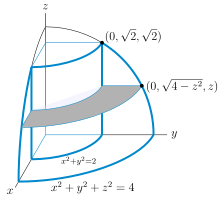
\includegraphics{cylSph.pdf}
\end{center}
So the cross-section has area 
$\pi\big(\sqrt{4-z^2}\big)^2-\pi\big(\sqrt{2}\big)^2=\pi\big(2-z^2\big)$
and
\begin{align*}
\tripInt_V\vnabla\cdot F\,\dee{V}
&=3\tripInt_V \,\dee{V}
=3\int_{-\sqrt{2}}^{\sqrt{2}} \pi\big(2-z^2\big)\,\dee{z}
=6\pi \int_{0}^{\sqrt{2}} \big(2-z^2\big)\,\dee{z}
=6\pi\big(2\sqrt{2}-\frac{2^{3/2}}{3}\big) \\
&=8\sqrt{2}\pi
\end{align*}

(c)
By the divergence theorem
$$
\dblInt_{S_2}\vF\cdot \hn\,\dee{S}
=\tripInt_V\vnabla\cdot F\,\dee{V}
-\dblInt_{S_1}\vF\cdot \hn\,\dee{S}
=16\sqrt{2}\pi
$$
\end{solution}


%%%%%%%%%%%%%%%%%%
\subsection*{\Application}
%%%%%%%%%%%%%%%%%%

\begin{question}
Let $\vE(\vr)$ be the electric field due to a charge
configuration that has density $\rho(\vr)$. Gauss' law states that, if
$V$ is any solid in $\bbbr^3$ with surface $\partial V$, then the electric
flux 
\begin{equation*}
\dblInt_{\partial V}\vE\cdot\hn\, \dee{S}=4\pi Q
\qquad{\rm where}\qquad Q=\tripInt_V\rho\ \dee{V}
\end{equation*}
is the total charge  in $V$. Here, as usual, $\hn$ is the outward pointing
unit normal to $\partial V$. Show that
\begin{equation*}
\vnabla\cdot\vE(\vr)=4\pi \rho(\vr)
\end{equation*}
for all $\vr$ in $\bbbr^3$. This is one of Maxwell's equations.
Assume that $\vnabla\cdot\vE(\vr)$ and $ \rho(\vr)$ are well--defined and continuous
everywhere.
\end{question}

\begin{hint} 
Review the derivation of the heat equation in Section \eref{CLP317}{sec:heatEqn}
of the CLP-4 text.
\end{hint}

\begin{answer} 
See the solution.
\end{answer}

\begin{solution} 
By the divergence theorem
\begin{equation*}
\dblInt_{\partial V}\vE\cdot\hn\, \dee{S}
=\tripInt_V\vnabla\cdot\vE\,\dee{V}
\end{equation*}
So by Gauss' law
\begin{equation*}
\tripInt_V\vnabla\cdot\vE\,\dee{V}=4\pi\tripInt_V\rho\ \dee{V}
\qquad\Rightarrow\qquad
\tripInt_V\big[\vnabla\cdot\vE-4\pi\rho\big]\,\dee{V}=0
\end{equation*}
This is true for all solids $V$ for which the divergence theorem applies.
If there were some point in $\bbbr^3$ for which $\vnabla\cdot\vE-4\pi\rho$
were, say, strictly bigger than zero, then, by continuity, we could find a ball
$B_\epsilon$ centered on that point with $\vnabla\cdot\vE-4\pi\rho>0$ everywhere
on $B_\epsilon$. This would force  $\tripInt_{B_\epsilon}\big[\vnabla\cdot\vE-4\pi\rho\big]\,\dee{V}>0$,
which violates $\tripInt_V\big[\vnabla\cdot\vE-4\pi\rho\big]\,\dee{V}=0$ with $V$
set equal to $B_\epsilon$. Hence $\vnabla\cdot\vE-4\pi\rho$ must be zero everywhere.
\end{solution}

%%%%%%%%%%%%%%%%%%%%%%%%%%%%%%%%
\begin{question}
Let $V$ be a solid in $\bbbr^3$ with surface $\partial V$.
Show that
\begin{equation*}
\dblInt_{\partial V}\vr\cdot\hn\,\dee{S}=3\,\text{Volume}(V)
\end{equation*}
where $\vr=x\,\hi+y\,\hj+z\,\hk$ and, as usual, $\hn$ is the outer 
normal to $\partial V$.
See if you can explain this result geometrically. 
\end{question}

%\begin{hint} 
%
%\end{hint}

\begin{answer} 
See the solution.
\end{answer}

\begin{solution} 
 By the divergence theorem
\begin{equation*}
\dblInt_{\partial V}\vr\cdot\hn\, \dee{S}
=\tripInt_V\vnabla\cdot\vr\,\dee{V}
=\tripInt_V\vnabla\cdot(x\,\hi+y\,\hj+z\,\hk)\,\dee{V}
=\tripInt_V 3\,\dee{V}
=3\,\text{Volume}(V)
\end{equation*}
Our gemetric explanation starts with the observation that
the volume of the cone with vertex $(0,0,0)$ and base a tiny piece of 
surface $\dee{S}$ is $\frac{1}{3}$ times the area of the base times 
the height of the cone. The height of the cone is $|\hn\cdot\vr|$, 
where $\vr$ is a point in $\dee{S}$. So the volume of the cone is $\frac{1}{3}|\hn\cdot\vr|\,\dee{S}$. 
\begin{center}
       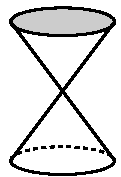
\includegraphics{cone.pdf}
\end{center}
First assume that $(0,0,0)$ is in $V$ and $V$ is convex.
Then 
\begin{itemize}\itemsep1pt \parskip0pt \parsep0pt %\itemindent-15pt
\item
$\hn\cdot\vr>0$, and the volume is  $\frac{1}{3} \hn\cdot\vr \,\dee{S}$. 
\item 
the cone is contained in $V$ and
\item
 $V$ is the union of all the tiny conical pieces
with $\dee{S}$ running over $\partial V$.
\end{itemize}
So
\begin{equation*}
\text{Volume}(V)=\frac{1}{3}\dblInt_{\partial V}\vr\cdot\hn\, \dee{S}
\end{equation*}
To generalise to the case that  $V$ is not convex or $(0,0,0)$ is not in $V$,
write $V$ as the difference between a large convex solid and one or more
smaller convex solids. 

\end{solution}

%%%%%%%%%%%%%%%%%%%%%%%%%%%%%%%%
\begin{question}[M317 2016A] %3
Let $S$ be the sphere of radius $3$, centered at the origin and 
with outward orientation. Given the vector field $\vF(x,y,z) = (0, 0, x + z)$:
\begin{enumerate}[(a)]
\item
Calculate (using the definition) the flux of $\vF$ through $S$
\begin{equation*}
   \dblInt_S \vF \cdot \hn\,\dee{S}
\end{equation*}
That is, compute the flux by evaluating the surface integral directly.

%\emph{Hint:} If you give a parametrization $\vr(\theta,\varphi)$ of the 
%sphere using the usual $\theta, \varphi$ of the spherical coordinates, 
%then $\vr_\theta\times\vr_\varphi$ and $\vr_\varphi\times\vr_\theta$ 
%both give a vector of the form $\alpha(\varphi)\vr(\theta, \varphi)$ 
%for some function $\alpha(\varphi)$. Determining which one to use is 
%important in the calculation above. Here, $\varphi$ is the angle 
%measured from the positive $z$-axis.
\item
   Calculate the same flux using the divergence theorem.
\end{enumerate}
\end{question}

\begin{hint} 
Make a judicious choice of parametrization.
\end{hint}

\begin{answer} 
(a), (b) $36\pi$
\end{answer}

\begin{solution} (a)
We'll parametrize the sphere using the spherical coordinates $\theta$ and
$\varphi$.
\begin{align*}
x&=3\sin\varphi\cos\theta \\
y&=3\sin\varphi\sin\theta \\
z&=3\cos\varphi
\end{align*}
with $0\le\theta\le 2\pi$, $0\le\varphi\le \pi$.
Since
\begin{align*}
\Big(\frac{\partial x}{\partial\theta}\,,\,
      \frac{\partial y}{\partial\theta}\,,\,
      \frac{\partial z}{\partial\theta}\Big)
&=\big(-3\sin\varphi\sin\theta\,,\,
       3\sin\varphi\cos\theta\,,\,0\big)\\
\Big(\frac{\partial x}{\partial\varphi}\,,\,\frac{\partial y}{\partial\varphi}
             \,,\, \frac{\partial z}{\partial\varphi}\Big)
&=(3\cos\varphi\cos\theta\,,\,3\cos\varphi\sin\theta\,,\,-3\sin\varphi) 
\end{align*}
(\eref{CLP317}{eq:SUdSparam}) in the CLP-4 text yields
\begin{align*}
\hn\,\dee{S}
&=\pm\Big(\frac{\partial x}{\partial\theta}\,,\,
          \frac{\partial y}{\partial\theta}\,,\,
          \frac{\partial z}{\partial\theta}\Big)
\times
\Big(\frac{\partial x}{\partial\varphi}\,,\,\frac{\partial y}{\partial\varphi}
   \,,\, \frac{\partial z}{\partial\varphi}\Big)
\ \dee{\theta}\dee{\varphi}\\
&=\pm \big(-3\sin\varphi\sin\theta\,,\,
       3\sin\varphi\cos\theta\,,\,0\big)
\times
(3\cos\varphi\cos\theta\,,\,3\cos\varphi\sin\theta\,,\,-3\sin\varphi)
\ \dee{\theta}\dee{\varphi}\\
&=\pm\big(-9\sin^2\varphi\cos\theta\,,\,
          -9\sin^2\varphi\sin\theta\,,\,
          -9\sin\varphi\cos\varphi\Big)\ \dee{\theta}\dee{\varphi} \\
&=\mp 9\sin\varphi \big(\sin\varphi\cos\theta\,,\,
          \sin\varphi\sin\theta\,,\,
          \cos\varphi\Big)\ \dee{\theta}\dee{\varphi} 
\end{align*}
To get an outward pointing normal we need the $+$ sign. For example, with the
$+$ sign, the $z$-component is $9\sin\varphi\cos\varphi
=\frac{9}{2}\sin(2\varphi)$ so that the normal is pointing upward when
$0<\varphi<\frac{\pi}{2}$, i.e. in the northern hemisphere,
and is pointing downward when $\frac{\pi}{2}<\varphi<\pi$, i.e.
in the southern hemisphere. (As a further consistency check, note that
$\hn(\theta,\varphi)$ is parallel to $\vr(\theta,\varphi)$.) So
\begin{align*}
\dblInt_S \vF \cdot \hn\,\dee{S}
&= 9\!\int_{0}^{2\pi}\hskip-10pt\dee{\theta}\!
\int_0^\pi\hskip-5pt\dee{\varphi}\,\sin\varphi\, 
(0,0,3\sin\varphi\cos\theta+3\cos\varphi)\!\cdot\!
\big(\sin\varphi\cos\theta\,,\,
          \sin\varphi\sin\theta\,,\,
          \cos\varphi\Big) \\
&= 27\int_{0}^{2\pi}\hskip-10pt\dee{\theta}
\int_0^\pi\hskip-5pt\dee{\varphi}\ \big(\sin^2\varphi\cos\varphi\cos\theta
                    +\sin\varphi\cos^2\varphi\big) \\
&= 54\pi\int_0^\pi\hskip-5pt\dee{\varphi}\ \sin\varphi\cos^2\varphi\qquad
\text{since $\int_0^{2\pi}\cos\theta\ \dee{\theta}=0$} \\
&= -18\pi \big[\cos^3\varphi\big]_0^\pi \\
&= 36\pi
\end{align*}

\noindent (b) 
Set
\begin{equation*}
V=\Set{(x,y,z)\in\bbbr^3}{x^2+y^2+z^2\le 9}
\end{equation*}
Since
\begin{equation*}
\vnabla\cdot\vF = \pdiff{}{z}\big(x+z\big)=1
\end{equation*}
the divergence theorem (Theorem \eref{CLP317}{thm:divThm} of the CLP-4 text) 
gives
\begin{equation*}
\dblInt_S \vF \cdot \hn\,\dee{S}
=\tripInt_V \vnabla\cdot\vF\,\dee{V}
=\tripInt_V \dee{V}
=\frac{4}{3}\pi 3^3
=36\pi
\end{equation*}
\end{solution}
%%%%%%%%%%%%%%%%%%%

\begin{question}[M317 2016A] %5
Consider the cube of side length $1$ that lies entirely in the first octant 
($x \ge 0$, $y \ge 0$, $z \ge 0$) with one corner at the origin and 
another corner at point $(1, 1, 1)$. As such, one face lies in the plane 
$x = 0$, one lies in the plane $y = 0$, and another lies in the plane $z = 0$. 
The other three faces lie in the planes $x = 1$, $y = 1$, and $z = 1$.
Denote $S$ as the open surface that consists of the union of the $5$ 
faces of the cube that do not lie in the plane $z = 0$. The surface $S$ 
is oriented in such a way that the unit normal vectors point outwards 
(that is, the orientation of $S$ is such that the unit normal
vectors on the top face point towards positive $z$-directions). 
Determine the value of
\begin{equation*}
I=\dblInt_S \vF \cdot\hn\, \dee{S} 
\end{equation*}
where $\vF$ is the vector field given by
\begin{equation*}
\vF = \left(y \cos(y^2) + z - 1\,,\, \frac{z}{x+1}+1\,,\, xy e^{z^2}\right)
\end{equation*}
%Hint: do not compute the integral directly. 
\end{question}

\begin{hint} 
Do not compute the integral directly.
\end{hint}

\begin{answer} 
$\frac{e}{4}$
\end{answer}

\begin{solution} 
Denote by $V$ the cube specified in the problem. Then $\partial V$
consists of $S$ together with the face $F$ in the plane $z=0$, oriented
with the normal being $-\hk$. 

\begin{center}
       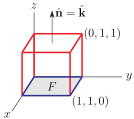
\includegraphics{cubeP.pdf}
\end{center}


\noindent 
As
\begin{align*}
\vnabla\cdot\vF &= 
    \pdiff{}{x}\big(y \cos(y^2) + z - 1\big)
     +\pdiff{}{y}\left(\frac{z}{x+1}+1\right)
     +\pdiff{}{z}\big(xy e^{z^2}\big) \\
   &=   \pdiff{}{z}\big(xy e^{z^2}\big) 
%   &=2xyz e^{z^2}
\end{align*}
the divergence theorem (Theorem \eref{CLP317}{thm:divThm} of the CLP-4 text) 
gives
\begin{align*}
\dblInt_S \vF \cdot \hn\,\dee{S}
&=\tripInt_V \vnabla\cdot\vF\,\dee{V}
    -\dblInt_F \vF \cdot (-\hk)\,\dee{S} \\
&=\int_0^1\dee{x}\int_0^1\dee{y}\int_0^1\dee{z}\ 
      \pdiff{}{z}\big(xy e^{z^2}\big)
  +\int_0^1\dee{x}\int_0^1\dee{y}\ xy e^{z^2}\Big|_{z=0} \\
&=\int_0^1\dee{x}\int_0^1\dee{y}\ xy e^{z^2}\Big|_{z=0}^{z=1}
+\int_0^1\dee{x}\int_0^1\dee{y}\ xy e^{z^2}\Big|_{z=0} \displaybreak[0]\\
&=\int_0^1\dee{x}\int_0^1\dee{y}\ xy e^{z^2}\Big|_{z=1} \displaybreak[0]\\
&=e\left[\frac{x^2}{2}\right]_0^1\ \left[\frac{y^2}{2}\right]_0^1 \\
&=\frac{e}{4}
\end{align*}

\end{solution}

%%%%%%%%%%%%%%%%%%%

\begin{question}[M317 2013D] %6

\begin{enumerate}[(a)]
\item
Find an upward pointing unit normal vector to the surface $z = xy$ at the 
point $(1, 1, 1)$.
\item
Now consider the part of the surface $z = xy$, which lies within the 
cylinder $x^2 + y^2 = 9$ and call it $S$. Compute the upward flux of 
$\vF = (y, x, 3)$ through $S$.
\item
Find the flux of $\vF = (y, x, 3)$ through the cylindrical surface 
$x^2 + y^2 = 9$ in between $z = xy$ and $z = 10$. The orientation is 
outward, away from the z-axis.
\end{enumerate}
\end{question}

\begin{hint} 
Be careful about which normals to use in part (c). For practice, try to do 
part (c) in two different ways, with one being direct evaluation.
\end{hint}

\begin{answer} 
(a) $\frac{1}{\sqrt{3}}(-1,-1,1)$\qquad
(b) $-\tfrac{27\pi}{2}$\qquad
(c) $-\tfrac{81\pi}{2}$
\end{answer}

\begin{solution}  (a)
The equation of the surface is $G(x,y,z)=z-xy=0$. So one normal to the
surface at $(1,1,1)$ is $(\vnabla G)(1,1,1)=(-y,-x,1)\big|_{(x,y,z)=(1,1,1)}
=(-1,-1,1)$ and a unit upward pointing normal at $(1,1,1)$ is
$\frac{(-1,-1,1)}{|(-1,-1,1)|}=\frac{1}{\sqrt{3}}(-1,-1,1)$.


\noindent (b)
For the surface $G(x,y,z)=z-xy$, so that, by (\eref{CLP317}{eq:SUdSimplicit})
in the CLP-4 text,
\begin{align*}
\hn\,\dee{S} =\pm\frac{\vnabla G(x,y,z)}{\vnabla G(x,y,z)\cdot\hk}\dee{x}\dee{y}
=\pm (-y,-x,1) \dee{x}\dee{y}
\end{align*}
The ``$+$'' sign gives the upward normal, so the specified upward flux is
\begin{align*}
\dblInt_S \vF\cdot\hn\,\dee{S}
=\dblInt_{x^2+y^2\le 9} (y,x,3)\cdot (-y-x,1)\,\dee{x}\dee{y}
=\dblInt_{x^2+y^2\le 9} (3-x^2-y^2)\,\dee{x}\dee{y}
\end{align*}
Switching to polar coordinates, the flux is
\begin{align*}
\dblInt_S \vF\cdot\hn\,\dee{S}
=\int_0^3\dee{r}\,r\int_0^{2\pi}\dee{\theta}\ (3-r^2)
=2\pi \int_0^3 \dee{r}\, (3r-r^3)
=2\pi \big(\tfrac{3}{2}3^2-\tfrac{1}{4}3^4\big)
=-\tfrac{27\pi}{2}
\end{align*}

\noindent (c) \emph{ by direct evaluation:}\ \ \ 
Parametrize the specified surface using the cylindrical coordinates $\theta$
and $z$.
\begin{align*}
x &= 3\cos \theta \\
y &= 3\sin \theta \\
z & = z 
\end{align*}
with $0\le\theta\le 2\pi$ and $9\sin\theta\cos\theta\le z\le 10$.
Then, using (\eref{CLP317}{eq:SUdSparam}) in the CLP-4 text,
\begin{align*}
\pdiff{\vr}{\theta}
 &= \big(-3\sin\theta\,,\, 3\cos\theta \,,\, 0\big) \\
\pdiff{\vr}{z}
 &= \big(0\,,\, 0 \,,\, 1\big) \\
\pdiff{\vr}{\theta} \times
     \pdiff{\vr}{z}
&=3\big(\cos\theta\,,\, \sin\theta\,,\,0 \big) \\
\hn\,\dee{S}
&= \pdiff{\vr}{\theta} \times
     \pdiff{\vr}{z}\dee{\theta}\,\dee{z}
=3\big(\cos\theta\,,\, \sin\theta\,,\,0 \big)\,\dee{\theta}\,\dee{z}
\end{align*}
(We have taken the $+$ sign in 
$\hn\,\dee{S}
= \pm \pdiff{\vr}{\theta} \times
     \pdiff{\vr}{z}\dee{\theta}\,\dee{z}$
to give the outward pointing normal.)
So the specified flux is
\begin{align*}
\dblInt \vF\cdot\hn\,\dee{S}
& = 3\int_0^{2\pi}\dee{\theta} \int_{9\cos\theta\sin\theta}^{10}\dee{z}\ 
     \overbrace{\big(3\sin\theta\,,\,3\cos\theta\,,\,3\big)}^{\vF=(y,x,3)}
        \cdot \big(\cos\theta\,,\, \sin\theta\,,\,0 \big) \\
& = 18\int_0^{2\pi}\dee{\theta} \int_{9\cos\theta\sin\theta}^{10}\dee{z}\ 
     \sin\theta\,\cos\theta \\
& = 18\int_0^{2\pi}\dee{\theta} \ 
     \big[10 -9\cos\theta\sin\theta\big]\sin\theta\,\cos\theta \\
& = -9\times 18\int_0^{2\pi}\dee{\theta}\ \sin^2\theta\,\cos^2\theta \\
&\qquad\qquad\text{since} \int_0^{2\pi} \sin\theta\cos\theta\ \dee{\theta}
                 =\frac{1}{2} \int_0^{2\pi}\sin(2\theta)\ \dee{\theta} = 0 \\
&=-9\times 18\times\frac{1}{4} \int_0^{2\pi}\dee{\theta}\ \sin^2(2\theta) \\
&=-\frac{81}{2}
          \int_0^{2\pi}\dee{\theta}\,\frac{1-\cos(4\theta)}{2} \\
&=-\frac{81}{2} 
     \left[\frac{\theta}{2}-\frac{\sin(4\theta)}{8}\right]_0^{2\pi} \\
&= -\frac{81}{2}\pi
\end{align*}
For an efficient, sneaky, way to evaluate 
$\int_0^{2\pi}\dee{\theta}\ \sin^2(2\theta)$ see Example
\eref{CLP317}{eg:workIntegalB} in the CLP-4 text.


\noindent (c) \emph{ using the divergence theorem:}\ \ \ 
Note that if $x^2+y^2\le 9$, then $|x|\le 3$ and $y\le 3$ so
that $|xy|\le 9<10$. Set
\begin{align*}
\tilde S&=\Set{(x,y,z)}{ x^2+y^2 = 9,\ xy\le z\le 10} \\
V&=\Set{(x,y,z)}{ x^2+y^2\le 9,\ xy\le z\le 10}
\end{align*}
Note that the boundary, $\partial V$,  of $V$ consists of three parts:
\begin{itemize}\itemsep1pt \parskip0pt \parsep0pt %\itemindent-15pt
\item[$\circ$]
the side $\tilde S$, with outward pointing normal (which is the surface and
the normal specified in part (c) of the question)
\item[$\circ$]
the bottom, which is the surface $S$ of part (b), with downward pointing
normal (which is opposite the normal specified in part (b)) and 
\item[$\circ$]
the top, which is the surface $S_T=\Set{(x,y,z)}{x^2+y^2\le 9,\ z=10}$,
with normal $\hn=\hk$.
\end{itemize} 
Here is a sketch of the part of $\partial V$ that is in the first octant.

\begin{center}
       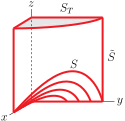
\includegraphics{OE13D_6.pdf}
\end{center}

\noindent
Note that $\vnabla\cdot\vF=0$. So the divergence theorem yields
\begin{align*}
0&=\tripInt_V \vnabla\cdot \vF\,\dee{V} \\
&=\dblInt_{\tilde \partial V} \vF\cdot\hn\,\dee{S} \\
&=\dblInt_{\tilde S} \vF\cdot\hn\,\dee{S}
   -\dblInt_{S} \vF\cdot\hn\,\dee{S}
   +\dblInt_{S_T} \vF\cdot\hk\,\dee{S} \\
\end{align*}
This implies
\begin{align*}
\dblInt_{\tilde S} \vF\cdot\hn\,\dee{S}
&=\dblInt_{S} \vF\cdot\hn\,\dee{S}
   -\dblInt_{S_T} \vF\cdot\hk\,\dee{S} \\
&=-\tfrac{27\pi}{2} -\dblInt_{x^2+y^2\le 9} 3\,\dee{S} \\
&= -\tfrac{27\pi}{2} -3 \pi 3^2
=-\tfrac{81\pi}{2}
\end{align*}
\end{solution}

%%%%%%%%%%%%%%%%%%%

\begin{question}[M317 2013D] %7

\begin{enumerate}[(a)]
\item
Find the divergence of the vector field $\vF  = (x + \sin y, z + y, z^2)$.
\item
Find the flux of $\vF$ through the upper hemisphere $x^2 + y^2 + z^2 = 25$, 
$z \ge 0$, oriented in the positive $z$-direction.
\item
Specify an oriented closed surface $S$, such that the flux 
$\dblInt_S\vF \cdot\hn\,\dee{S}$ is equal to $-9$.
\end{enumerate}
\end{question}

\begin{hint} 
For part (b), do not evaluate the flux directly.
In part (c), the flux can be related to the volume enclosed by the
surface, and the centre of mass of the volume enclosed by the surface.

\end{hint}

\begin{answer} 
(a) $\vnabla\cdot\vF =2+2z$\qquad
(b) $\pi\frac{23}{6} 5^3 =\frac{2875}{6}\pi$  

(c) Let $S$ be an oriented surface that encloses a solid $V$ and has outward pointing normal. If $\bar z = -\frac{9}{2|V|}-1$, where $|V|$ is the 
volume of $V$ and $\bar z$ is the $z$-component of the centroid
(i.e. centre of mass with constant density) of $V$, then 
$\dblInt_{S} \vF\cdot\hn\,\dee{S}=-9$. One surface which obeys 
this condition is the unit cube (with outward normal)
centred on $\big(0,0, -\frac{11}{2}\big)$.
\end{answer}

\begin{solution} (a)
The divergence of $\vF$ is
\begin{align*}
\vnabla\cdot\vF 
&= \tfrac{\partial\hfill}{\partial x}(x+\sin y)
  +\tfrac{\partial\hfill}{\partial y}(z+y)
  +\tfrac{\partial\hfill}{\partial z}(z^2) \\
&=2+2z
\end{align*}

\noindent (b) Set
\begin{align*}
V &= \Set{(x,y,z)}{x^2+y^2\le 25,\ 0\le z\le \sqrt{25-x^2-y^2}} \\
S_T &= \Set{(x,y,z)}{x^2+y^2+z^2 = 25,\ z\ge 0} \\
S_B &= \Set{(x,y,z)}{x^2+y^2 \le 25,\ z= 0} 
\end{align*}
Note that the boundary, $\partial V$, of $V$ consists ot two parts ---
$S_T$ with upward normal, and $S_B$ with normal $-\hk$.
We are to find the flux through $S_T$ with upward normal. By the 
divergence theorem, it is
\begin{align*}
\dblInt_{S_T} \vF\cdot\hn\,\dee{S}
&=\tripInt_V \vnabla\cdot\vF\,\dee{V} 
     - \dblInt_{S_B} \vF\cdot(-\hk)\,\dee{S} \\
&= \tripInt_V (2+2z)\,\dee{V}  
\end{align*} 
since $\vF\cdot\hk=z^2=0$ on $S_B$. We'll compute the volume integral by expressing it as an iterated integral, with the $z$ integration on the 
outside. In $V$, $z$ ranges for $0$ to $5$. The set of points 
at exactly height $z$ in $V$ is  $\Set{(x,y,z)}{x^2+y^2\le 25-z^2}$. 
So
\begin{align*}
\dblInt_{S_T} \vF\cdot\hn\,\dee{S}
&= \int_0^5\dee{z}\hskip-10pt \dblInt_{x^2+y^2\le 25-z^2}\hskip-15pt 
            \dee{x}\,\dee{y}\  (2+2z)
= \int_0^5\dee{z}\ (2+2z)\hskip-10pt\dblInt_{x^2+y^2\le 25-z^2}\hskip-15pt 
\dee{x}\,\dee{y} \\
&= \int_0^5\dee{z}\ \pi(25-z^2) (2+2z) \\
\intertext{since $\dblInt_{x^2+y^2\le 25-z^2} \dee{x}\,\dee{y}$
is the area of a disk of radius $\sqrt{25-z^2}$}
&= \pi\int_0^5\dee{z}\ (50 -2z^2 +50z -2z^3) \\
&=\pi\Big(50\times 5-2\frac{5^3}{3} +50\frac{5^2}{2}-2\frac{5^4}{4}\Big)
=\pi 5^3 \Big(2-\frac{2}{3} +5-\frac{5}{2}\Big) 
= \pi\,5^3 \Big(\frac{4}{3}+\frac{5}{2}\Big) \\
&=\pi\frac{23}{6} 5^3
=\frac{2875}{6}\pi
\end{align*}

\noindent (c)
To start, consider any closed surface $S$ that is the boundary of a
solid $V$. Use 
\begin{itemize}\itemsep1pt \parskip0pt \parsep0pt %\itemindent-15pt
\item[$\circ$]
the outward pointing normal for $S$, 
\item[$\circ$]
$|V|$ to denote the volume of $V$, and
\item[$\circ$] 
$\bar z=\frac{1}{|V|}\tripInt_V z\ \dee{V}$ to denote the $z$-component 
of the centroid (i.e. centre of mass with constant density) of $V$.
\end{itemize}
Then, by the divergence theorem
\begin{align*}
\dblInt_{S} \vF\cdot\hn\,\dee{S}
&=\tripInt_V \vnabla\cdot\vF\,\dee{V}
=\tripInt_V (2+2z)\,\dee{V}
=2\tripInt_V \,\dee{V} +2\tripInt_V z\,\dee{V} \\
&=2|V| +2|V|\bar z
\end{align*}
This takes the value $-9$ if and only if
\begin{align*}
 2|V|\bar z =-9-2|V| \iff
\bar z = -\frac{9}{2|V|}-1
\end{align*}
One surface which obeys this condition is the unit cube (with outward normal)
centred on $\big(0,0, -\frac{11}{2}\big)$.


\end{solution}

%%%%%%%%%%%%%%%%%%%%%%%%%%%
\begin{question}[M317 2011D] %7
Evaluate the surface integrals. (Use any method you like.)
\begin{enumerate}[(a)]
\item
$\dblInt_S z^2\,\dee{S}$, if $S$ is the part of the cone 
$x^2 + y^2 = 4z^2$ where $0 \le x \le y$ and $0 \le z \le 1$.

\item
$\dblInt_S \vF \cdot \hn\,\dee{S}$, if $\vF = z\hk$ and $S$ is the rectangle 
with vertices $(0, 2, 0)$, $(0, 0, 4)$, $(5, 2, 0)$, $(5, 0, 4)$, oriented 
so that the normal vector points upward.

\item
$\dblInt_S \vF \cdot \hn\,\dee{S}$, where $\vF = (y - z^2 )\hi + (z - x^2)\hj 
+ z^2\hk$ and $S$ is the boundary surface
of the box $0 \le x \le 1$, $0 \le y \le 2$, $0 \le z \le 3$, 
with the normal vector pointing outward.
\end{enumerate}
\end{question}

\begin{hint} 
(b) We have several different methods for evaluating flux integrals.
Think about what would be involved in applying each of them before 
settling on which one to use.

(c) Be sneaky --- don't evaluate this integral directly.
\end{hint}

\begin{answer} 
(a) $\frac{\sqrt{5}\pi}{8}$ \qquad
(b) $20$ \qquad
(c) $18$
\end{answer}

\begin{solution} (a) The constant $z$ cross-section of the cone at height
$0\le z\le 1$ is a circle of radius $2z$. So we may parametrize the
cone by
\begin{equation*}
\vr(\theta,z) = 2z\cos\theta\,\hi + 2z\sin\theta\,\hj +z\,\hk
\qquad 0\le\theta< 2\pi,\ 0\le z\le 1
\end{equation*}
Since
\begin{align*}
\tfrac{\partial\vr}{\partial\theta}
&=\big(-2z\sin\theta\,,\,
        2z\cos\theta\,,\,
          0 \big) \\
\tfrac{\partial\vr}{\partial z}
&=\big(2\cos\theta\,,\,
       2\sin\theta\,,\,
          1 \big) \\
\tfrac{\partial\vr}{\partial\theta} \times \tfrac{\partial\vr}{\partial z} 
&=\big(2z\cos\theta\,,\,
       2z\sin\theta\,,\,
       -4z\big)
\end{align*}
(\eref{CLP317}{eq:SUdSparam}) in the CLP-4 text yields that
the element of surface area for this parametrization is
\begin{align*}
\dee{S} &= 
\big|\tfrac{\partial\vr}{\partial\theta}\times
      \tfrac{\partial\vr}{\partial z} \big|\dee{\theta}\dee{z}
\ =\ 2z\big|(\cos\theta\,,\,\sin\theta\,,\,-2\big)\big|
    \dee{\theta}\dee{z} \\ 
&=2\sqrt{5}z\,\dee{\theta}\dee{z}
\end{align*}
In our parametrization the condition $x\le y$ becomes
$2z\cos\theta\le 2z\sin\theta$, which, for $z> 0$, is equivalent
to $\tan\theta\ge 1$.
So the specified integral is
\begin{align*}
\dblInt_S z^2\,\dee{S}
&=2\sqrt{5}\int_0^1\dee{z}\int_{\pi/4}^{\pi/2}\dee{\theta}\ z^3
=\frac{\sqrt{5}\pi}{2}\int_0^1\dee{z}\ z^3
=\frac{\sqrt{5}\pi}{8}
\end{align*}

\noindent (b) Let's first do some strategizing. We have to compute a flux integral over a surface that is not closed. There are two potential sneaky
attacks that come to mind.
\begin{itemize}\itemsep1pt \parskip0pt \parsep0pt %\itemindent-15pt
\item[$\circ$] The first uses Stokes' theorem. But the flux integral 
in Stokes' theorem  is of the form 
$\dblInt_S \vnabla\times\vA\cdot\hn\,\dee{S}$. So to be able to apply
Stokes' theorem in the current problem, $\vF$ has to be of the form
$\vnabla\times\vA$. That is, $\vF$ has to have a vector potential.
We know that in order for $\vF$ to have a vector potential, it must 
pass the screening test $\vnabla\cdot\vF=0$. Our $\vF=z\,\hk$ fails
this screening test. So we can't use Stokes' theorem.

\item[$\circ$] The second uses the divergence theorem. But the flux
integral in the divergence theorem is over the boundary of a solid.
That is not the case for our $S$. So in order to apply the divergence theorem
in the current problem, we have to enlarge $S$ to the boundary of
a solid. There are many ways to do this. But they all appear
fairly complicated. So it does not seem wise to use the divergence theorem.
\end{itemize}
So it looks like we have to evaluate the flux integral directly.
To do so, we have to determine $\hn\,\dee{S}$ for the specified rectangle.
Look at the sketch of $S$ below. It is part of a plane,
\vadjust{
\begin{center}
       \includegraphics{OE11D_7.pdf}
\end{center}
}
and that plane is invariant under translations parallel to the
$x$ axis. As the plane does not pass through the origin, the equation
of the plane has to be of the form $by+cz=1$. For $(0,0,4)$ to be on the plane,
we need $c=\frac{1}{4}$. For $(0,2,0)$ to be on the plane, we need
$b=\frac{1}{2}$. So $S$ is contained in the plane 
$G(x,y,z) = \frac{y}{2} +\frac{z}{4} =1$ and 
equation (\eref{CLP317}{eq:SUdSimplicit}) in the CLP-4 text gives that
\begin{equation*}
\hn\,\dee{S} = \pm\frac{\vnabla G(x,y,z)}{\vnabla G(x,y,z)\cdot\hk}
                       \dee{x}\dee{y}
=\pm \frac{(0,\nicefrac{1}{2},\nicefrac{1}{4})}{\nicefrac{1}{4}} \dee{x}\dee{y}
=\pm (0,2,1)\, \dee{x}\dee{y}
\end{equation*}
The problem specifies that the normal is to be upward, i.e. is to have
a positive $z$-component. So
\begin{equation*}
\hn\,\dee{S} = (0,2,1)\,\dee{x}\dee{y}
\end{equation*}
Again looking at the sketch of $S$ above we see, as $(x,y,z)$ runs over $S$, $(x,y)$ runs over
\begin{equation*}
R = \Set{(x,y)}{0\le x\le 5,\ 0\le y\le 2}
\end{equation*}
Thus our flux integral is
\begin{align*}
\dblInt_S \vF \cdot \hn\,\dee{S}
&=\dblInt_R \overbrace{\big(4-2y\big)}^{z}\hk\cdot 
           \overbrace{(0,2,1)\,\dee{x}\dee{y}}^{\hn\,\dee{S}}
=\int_0^2\dee{y}\int_0^5\dee{x}\ (4-2y) \\
&= \int_0^2\dee{y}\ 5(4-2y)
=5\Big[4y-y^2\Big]_0^2
=20
\end{align*}



\noindent (c) The divergence of the given vector field is
$\vnabla\cdot\vF = 2z$, which is pretty simple. So let's
use the divergence theorem. If 
$V=\Set{(x,y,z)}{0 \le x \le 1$, $0 \le y \le 2$, $0 \le z \le 3}$,
the divergence theorem says that
\begin{align*}
\dblInt_S \vF \cdot \hn\,\dee{S}
&= \tripInt_V \vnabla\cdot\vF\,\dee{V}
= 2\tripInt_V z\,\dee{V}
\end{align*}
This integral would be easy enough to evaluate directly, but we don't
need to. The average value of $z$ (i.e. the $z$-coordinate of the centre
of mass with constant density) is $\frac{3}{2}$, by symmetry. Since $V$
has volume $6$, that average value of $z$ is also
\begin{align*}
\bar z = \frac{1}{6} \tripInt_V z\,\dee{V} = \frac{3}{2}
\end{align*}
So $\tripInt_V z\,\dee{V}=9$
\begin{align*}
\dblInt_S \vF \cdot \hn\,\dee{S}
= 2\tripInt_V z\,\dee{V}
=18
\end{align*}


\end{solution}

%%%%%%%%%%%%%%%%%%%%%%%%%%%
\begin{question}[M317 2010A] %5
Let $\sigma_1$ be the open surface given by $z = 1 - x^2 - y^2$, $z \ge 0$. 
Let $\sigma_2$ be the open surface given by $z = x^2 + y^2 - 1$, $z \le 0$. 
Let $\sigma_3$ be the planar surface given by $z = 0$, 
$x^2 + y^2 \le 1$. 
Let $\vF = [ a ( y^2 + z^2 ) + bxz ]\,\hi 
          + [ c ( x^2 + z^2 ) + dyz ]\,\hj 
          + x^2\,\hk$
where $a$, $b$, $c$, and $d$ are constants.
\begin{enumerate}[(a)]
\item
Find the flux of $\vF$ upwards across $\sigma_1$.
\item
Find all values of the constants $a$, $b$, $c$, and $d$ so that the 
flux of $\vF$ outwards across the closed surface $\sigma_1 \cup \sigma_3$ 
is zero.
\item
Find all values of the constants $a$, $b$, $c$, and $d$ so that the 
flux of $\vF$ outwards across the closed surface $\sigma_1 \cup \sigma_2$ 
is zero.

\end{enumerate}
\end{question}

\begin{hint} 
For parts (b) and (c), write out carefully the integral that the
divergence theorem gives you.
\end{hint}

\begin{answer} 
(a) $\frac{\pi}{4} +\frac{\pi(b+d)}{6}$

(b) $\dblInt_{\sigma_1\cup\sigma_3} \vF\cdot\hn\,\dee{S}$ is zero 
if and only if $d=-b$.

(c) $\dblInt_{\sigma_1\cup\sigma_3} \vF\cdot\hn\,\dee{S}$ is zero 
  for all $a$, $b$, $c$, $d$.
\end{answer}

\begin{solution} (a) For the surface $z=f(x,y)=1-x^2-y^2$, with an upwards
pointing normal,
\begin{equation*}
\hn\,\dee{S} = \big[-f_x(x,y)\,\dee{x} -f_y(x,y) +\hk\big]\dee{x}\dee{y}
             = \big[2x\,\hi + 2y\,\hj +\hk\big]\,\dee{x}\dee{y}
\end{equation*}
by (\eref{CLP317}{eq:SUdSgraph}) in the CLP-4 text.
So the specified upward flux is
\begin{align*}
&\dblInt_{\sigma_1} \vF\cdot\hn\,\dee{S} \\
&\hskip0.5in=\dblInt_{x^2+y^2\le 1}\hskip-5pt
         \big\{[ a ( y^2 + z^2 ) + bxz ]\,\hi 
          + [ c ( x^2 + z^2 ) + dyz ]\,\hj + x^2\,\hk\big\}\\
&\hskip3.8in\cdot
            \big\{2x\,\hi + 2y\,\hj +\hk\big\}_{z=1 - x^2 - y^2}
         \,\dee{x}\dee{y} \\
&\hskip0.5in=\!\dblInt_{x^2+y^2\le 1}\hskip-5pt
         \big\{[2a x( y^2 \!+\! z^2 ) + 2bx^2z ]
          + [2cy ( x^2 \!+\! z^2 ) +2 dy^2z ] + x^2\big\}_{z=1 - x^2 - y^2}
         \,\dee{x}\dee{y} \\
\end{align*}
Now
\begin{equation*}
\dblInt_{x^2+y^2\le 1}\hskip-5pt
         \big\{2a x( y^2 + z^2 ) \big\}_{z=1 - x^2 - y^2}
         \,\dee{x}\dee{y} =0
\end{equation*}
because the integrand is odd under $x\rightarrow -x$ and
\begin{equation*}
\dblInt_{x^2+y^2\le 1}\hskip-5pt
         \big\{2cy ( x^2 + z^2 )\big\}_{z=1 - x^2 - y^2}
         \,\dee{x}\dee{y} =0 
\end{equation*}
because the integrand is odd under $y\rightarrow -y$. So that leaves
\begin{equation*}
\dblInt_{\sigma_1} \vF\cdot\hn\,\dee{S}
=\dblInt_{x^2+y^2\le 1}\hskip-5pt
         \big\{ 2bx^2z +2 dy^2z  + x^2\big\}_{z=1 - x^2 - y^2}
         \,\dee{x}\dee{y}
\end{equation*}
We'll switch to polar coordinates to evaluate the remaining integral.
\begin{align*}
\dblInt_{\sigma_1} \vF\cdot\hn\,\dee{S}
&=\int_0^1\dee{r}\, r\int_0^{2\pi}\dee{\theta}\ 
         \big\{ 2br^2z\cos^2\theta  +2 dr^2z\sin^2\theta 
                     + r^2\cos^2\theta\big\}_{z=1 - r^2}
\end{align*}
Now
\begin{align*}
\int_0^{2\pi}\cos^2\theta\ \dee{\theta}
&=\int_0^{2\pi}\frac{\cos(2\theta)+1}{2}\ \dee{\theta}
=\left[\frac{\sin(2\theta)}{4}+\frac{\theta}{2}\right]_0^{2\pi}
=\pi
\\
\int_0^{2\pi}\sin^2\theta\ \dee{\theta}
&=\int_0^{2\pi}\frac{1-\cos(2\theta)}{2}\ \dee{\theta}
=\left[\frac{\theta}{2}-\frac{\sin(2\theta)}{4}\right]_0^{2\pi}
=\pi
\end{align*}
For an efficient, sneaky, way to evaluate 
$\int_0^{2\pi} \cos^2\theta\,\dee{\theta}$ 
and $\int_0^{2\pi} \sin^2\theta\,\dee{\theta}$,
see Example
\eref{CLP317}{eg:workIntegalB} in the CLP-4 text.
So, we finally have
\begin{align*}
\dblInt_{\sigma_1} \vF\cdot\hn\,\dee{S}
&=\int_0^1\dee{r}\,  
         \big\{ 2\pi br^3(1-r^2)  +2\pi dr^3(1-r^2) 
                     + \pi r^3\big\} \\
&=2\pi b\Big[\frac{1}{4}-\frac{1}{6}\Big]
  +2\pi d\Big[\frac{1}{4}-\frac{1}{6}\Big]
  +\pi\frac{1}{4}
=\frac{\pi}{4} +\frac{\pi(b+d)}{6}
\end{align*}

(b), (c) Here is a side view of $\sigma_1$, $\sigma_2$ and $\sigma_3$.
\begin{center}
  \includegraphics{OE10A_5.pdf}
\end{center}
Set
\begin{align*}
V_b &=\Set{(x,y,z)}{0\le z \le 1-x^2-y^2,\ x^2+y^2\le 1} \\
V_c &=\Set{(x,y,z)}{x^2+y^2-1 \le z \le 1-x^2-y^2,\ x^2+y^2\le 1} 
\end{align*}
Then $\partial V_b = \sigma_1\cup\sigma_3$ and 
     $\partial V_c = \sigma_1\cup\sigma_2$,
all with outward pointing normals. Since the divergence of $\vF$ is
\begin{equation*}
\vnabla\cdot\vF = 
  \pdiff{}{x}[ a ( y^2 + z^2 ) + bxz ]
  +\pdiff{}{y}[ c ( x^2 + z^2 ) + dyz ]
  +\pdiff{}{z}[ x^2]
= (b+d) z
\end{equation*}
the divergence theorem gives
\begin{align*}
\dblInt_{\sigma_1\cup\sigma_3} \vF\cdot\hn\,\dee{S}
   & = \tripInt_{V_b} \vnabla\cdot\vF\,\dee{V}
     = (b+d)\tripInt_{V_b} z\,\dee{V} \\
\dblInt_{\sigma_1\cup\sigma_2} \vF\cdot\hn\,\dee{S}
   & = \tripInt_{V_c} \vnabla\cdot\vF\,\dee{V}
     = (b+d)\tripInt_{V_c} z\,\dee{V} \\
\end{align*}
Now on $V_b$, $z\ge 0$ and $z>0$ except on $\sigma_3$. So 
$\tripInt_{V_b} z\,\dee{V}>0$ and 
$\dblInt_{\sigma_1\cup\sigma_3} \vF\cdot\hn\,\dee{S}$ is zero if and only if 
$d=-b$. That's the answer to part (b).


On the other hand,  $V_c$ is even under $z\rightarrow -z$ so that 
$\tripInt_{V_c} z\,\dee{V}=0$. Consequently
$\dblInt_{\sigma_1\cup\sigma_3} \vF\cdot\hn\,\dee{S}$ is zero for all $a$, $b$,
$c$, $d$.  That's the answer to part (c).

\end{solution}

%%%%%%%%%%%%%%%%%%%%%%%%%%%
\begin{question}[M317 2005A] %3
Let $S$ be the ellipsoid $x^2+2y^2+3z^2=16$ and $\hn$ its outward unit 
normal.
\begin{enumerate}[(a)]
\item
Find $\dblInt_S \vF\cdot\hn\,\dee{S}$ if
$\vF(x,y,z)=\dfrac{(x,y,z)-(2,1,1)}{{\big[(x-2)^2+(y-1)^2+(z-1)^2\big]}^{3/2}}$.
\item
Find $\dblInt_S \vG\cdot\hn\,\dee{S}$ if
$\vG(x,y,z)=\dfrac{(x,y,z)-(3,2,2)}{{\big[(x-3)^2+(y-2)^2+(z-2)^2\big]}^{3/2}}$.
\end{enumerate}
\end{question}

\begin{hint} 
Note that $2^2+2(1^2)+3(1)^2 = 9<16$ so that $(2,1,1)$ is inside $S$,\\
while $3^2+2(2^2)+3(2)^2 = 29>16$ so that $(3,2,2)$ is outside $S$.
\end{hint}

\begin{answer} 
(a) $4\pi$  \qquad
(b) $0$.
\end{answer}

\begin{solution}
We will be using the divergence theorem in both parts (a) and $b$. 
So as a prelimary calculation, let's find the divergence of
$\vH(x,y,z)=\frac{(x,y,z)-(a,b,c)}{{[(x-a)^2+(y-b)^2+(z-b)^2]}^{3/2}}$
for any $(a,b,c)$. If $(x,y,z)\ne(a,b,c)$,
\begin{align*}
&\vnabla\cdot\vH(x,y,z) \\
&\hskip0.25in
=\pdiff{}{x}\frac{x-a}
               {{[(x-a)^2+(y-b)^2+(z-c)^2]}^{3/2}}
+\pdiff{}{y}\frac{y-b}
               {{[(x-a)^2+(y-b)^2+(z-c)^2]}^{3/2}} \\&\hskip2in
+\pdiff{}{z}\frac{z-c}
                {{[(x-a)^2+(y-b)^2+(z-c)^2]}^{3/2}}
\\
&\hskip0.25in
=\frac{\big[(x-a)^2+(y-b)^2+(z-c)^2\big]\ -\ (x-a)\ \frac{3}{2}(2(x-a))}
                       {{\big[(x-a)^2+(y-b)^2+(z-c)^2\big]}^{5/2}}
   \\&\hskip2in
+\frac{\big[(x-a)^2+(y-b)^2+(z-c)^2\big]\ -\ (y-b)\ \frac{3}{2}(2y)}
                        {{\big[(x-a)^2+(y-b)^2+(z-c)^2\big]}^{5/2}}
    \\&\hskip2in
+\frac{\big[(x-a)^2+(y-b)^2+z^2\big]\ -\ (z-c)\ \frac{3}{2}(2(z-c))}
                       {{\big[(x-a)^2+(y-b)^2+(z-c)^2\big]}^{5/2}}
\\
&\hskip0.25in
=\frac{3\big[(x-a)^2+(y-b)^2+(z-c)^2\big]\ -\ 3(x-a)^2-3(y-b)^2-3(z-c)^2}
                       {{\big[(x-a)^2+(y-b)^2+(z-c)^2\big]}^{5/2}} \\
&\hskip0.25in=0
\end{align*}
If $(x,y,z)=(a,b,c)$, $\vH(x,y,z)$ is not defined 
and hence $\vnabla\cdot\vH(x,y,z)$ is also not defined.

(b) By the above preliminary computation with $(a,b,c)=(3,2,2)$, 
$\vnabla\cdot\vG$ is defined and zero for all $(x,y,z)\ne (3,2,2)$,
and, in particular for all $(x,y,z)$ in
\begin{equation*}
V=\Set{(x,y,z)}{x^2+2y^2+3z^2\le 16}
\end{equation*}
So, by the divergence theorem,
\begin{align*}
\dblInt_S \vG\cdot\hn\,\dee{S}
&=\tripInt_V\vnabla\cdot\vG\,\dee{V}
=0
\end{align*}

(a) Because $(1,1,2)$ is inside $V$, we cannot use the argument of part (b),
to conclude that the integral is zero. Let $\veps>0$ be small enough
that
\begin{equation*}
S_\veps = \Set{(x,y,z)}{(x-2)^2 + (y-1)^2 +(z-1)^2=\veps^2}
\end{equation*}
is completely contained inside $V$, as in the sketch below.

\begin{center}
       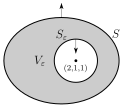
\includegraphics{OE05A_3.pdf}
\end{center}

\noindent Set
\begin{equation*}
V_\veps=\Set{(x,y,z)}{x^2+2y^2+3z^2\le 16,\ 
                (x-2)^2 + (y-1)^2 +(z-1)^2\ge\veps^2}
\end{equation*}
The boundary, $\partial V_\veps$, of $V$ consists of two parts ---
$S$ and $S_\veps$, with the normals as in the figure above. The divergence
$\vnabla\cdot\vF$ of $\vF$ is well-defined and zero throughout $V_\veps$.
Consequently, the divergence theorem gives
\begin{align*}
0 &= \tripInt_V\vnabla\cdot\vF\,\dee{V}
   = \dblInt_S \vF\cdot\hn\,\dee{S} 
      + \dblInt_{S_\veps} \vF\cdot\hn\,\dee{S}
\end{align*}
So
\begin{equation*}
\dblInt_S \vF\cdot\hn\,\dee{S} = -\dblInt_{S_\veps} \vF\cdot\hn\,\dee{S}
\end{equation*}
The unit normal to $S_\veps$ at the point $(x,y,z)$ on $S_\veps$ is
\begin{equation*}
\hn =-\frac{1}{\veps}\big[(x-2)\,\hi + (y-1)\,\hj +(z-1)\,\hk\big]
\end{equation*}
(Recall that $|(2-1)\,\hi + (y-1)\,\hj +(z-1)\,\hk|=\veps$ on $S_\veps$.
So, on $S_\veps$,
\begin{align*}
\vF\cdot\hn 
&= -\frac{1}{\veps}
  \left(\frac{(x,y,z)-(2,1,1)}{{\big[(x-2)^2+(y-1)^2+(z-1)^2\big]}^{3/2}}\right)
  \cdot\big[(x-2)\,\hi + (y-1)\,\hj +(z-1)\,\hk\big] \\
&=-\frac{1}{\veps} \left(\frac{(x-2)^2+(y-1)^2+(z-1)^2}{{\big[(x-2)^2+(y-1)^2+(z-1)^2\big]
                                                        }^{3/2}}\right)\\
&= -\frac{1}{\veps^2}
\end{align*}
Hence
\begin{align*}
\dblInt_S \vF\cdot\hn\,\dee{S} 
= -\dblInt_{S_\veps}   \left(-\frac{1}{\veps^2}\right)\,\dee{S}
=\frac{1}{\veps^2} (4\pi\veps^2)
=4\pi
\end{align*}

\end{solution}
%%%%%%%%%%%%%%%%%%%

%%%%%%%%%%%%%%%%%%%%%%%%%%%
\begin{question}[M317 2005A] %7
Let $\Om\subset\bbbr^3$ be a smoothly bounded domain, with boundary $\partial\Om$ and outer unit normal $\hn$. Prove that for any vector field $\vF$ which is continuously differentiable in $\Om\cup\partial\Om$,
\begin{equation*}
\tripInt_\Om \vnabla\times\vF\,\dee{V}
   = -\dblInt_{\partial\Om} \vF\times\hn\,\dee{S}
\end{equation*}
\end{question}

\begin{hint} 
Review \S\eref{CLP317}{sec:divVar} in the CLP-4 text.
\end{hint}

\begin{answer} 
See the solution.
\end{answer}

\begin{solution}
This was part of Theorem \eref{CLP317}{thm:divVrn} in the CLP-4 text. 
To prove it apply the divergence theorem, but with
$\vF$ replaced by $\va\times\vF$, where $\va$ is any constant vector.
\begin{align*}
&\dblInt_{\partial \Omega} (\va\times\vF)\cdot\hn\ \dee{S}
=\tripInt_V\vnabla\cdot(\va\times\vF)\ \dee{V} \\
&\hskip0.5in
=\tripInt_\Omega\big[\vF\cdot\underbrace{(\vnabla \times \va)}_{=\vZero}
  -\va\cdot(\vnabla\times\vF)\big]\ \dee{V}  \\
&\hskip0.5in=-\tripInt_\Omega\va\cdot(\vnabla \times\vF)\ \dee{V}
=-\va\cdot\tripInt_\Omega\vnabla \times\vF\ \dee{V}
\end{align*}
To get the second line we used the vector identity Theorem \eref{CLP317}{thm:divIdentities}.d in the CLP-4 text.
To get the third line, we used that $\va$ is a constant, so that
all of its derivatives are zero. For all vectors 
$\va\cdot(\vb\times\vc)=(\va\times\vb)\cdot\vc$ (in case you don't
remember this, it was Lemma \eref{CLP317}{lem:tripProd}.a in the CLP-4 text) 
so that
\begin{equation*}
(\va\times\vF)\cdot\hn
=\va\cdot(\vF\times\hn)
\end{equation*}
and
\begin{align*}
&\va\cdot\dblInt_{\partial \Omega} \vF\times\vn\ \dee{S}
=-\va\cdot\tripInt_\Omega\vnabla \times\vF\ \dee{V} \\
\implies &\va\cdot\bigg\{\dblInt_{\partial \Omega} \vF\times\vn\ \dee{S}
+\tripInt_\Omega\vnabla\times\vF\ \dee{V}\bigg\}=0
\end{align*}
In particular, choosing $\va=\hi$, $\hj$ and $\hk$, we see that
all three components of the vector 
$\dblInt_{\partial \Omega} \vF\times\vn\ \dee{S}
+\tripInt_\Omega\vnabla\times\vF\ \dee{V}$ are zero. So 
\begin{equation*}
\tripInt_\Omega\vnabla\times\vF\ \dee{V}
=-\dblInt_{\partial \Omega} \vF\times\vn\ \dee{S}
=\dblInt_{\partial \Omega} \hn\times\vF\ \dee{S}
\end{equation*}
which is what we wanted show.
\end{solution}

%%%%%%%%%%%%%%%%%%%%%%%%%%%
\begin{question}[M317 2004A] %4
Recall that if $S$ is a smooth closed surface with outer
normal field $\hn$, then for any smooth function $p(x,y,z)$ on $\bbbr^3$,
we have
\begin{equation*}
\dblInt_S p\hn\ \dee{s}=\tripInt_E \nabla p\ \dee{V}
\end{equation*}
where $E$ is the solid bounded by $S$. Show that as a consequence,
the total force exerted on the surface of a solid body contained in a gas
of constant pressure is zero. (Recall that the pressure acts in the direction
normal to the surface.)
\end{question}

%\begin{hint} 
%\end{hint}

\begin{answer} 
See the solution.
\end{answer}

\begin{solution} 
Pressure is force per unit surface area acting normally into
a surface. So the force per unit surface area is $-p\hn$. The total force
acting on $S$ is
\begin{equation*}
-\dblInt_S p\hn\,\dee{S}=-\tripInt_E \nabla p\ \dee{V}
\end{equation*}
We are assuming that $p$ is a constant, so that $\nabla p=0$ and the 
total force is zero.
\end{solution}

%%%%%%%%%%%%%%%%%%%%%%%%%%%
\begin{question}[M317 2002A] %8
Let $\vF$ be a smooth 3-dimensional
vector field such that the flux of $\vF$ out of the sphere $x^2+y^2+z^2=a^2$
is equal to $\pi(a^3+2a^4)$ for every $a>0$. 
Calculate $\vnabla\cdot \vF(0,0,0)$.
\end{question}

\begin{hint} 
Consider very small $a$'s.
\end{hint}

\begin{answer} 
$\frac{3}{4}$
\end{answer}

\begin{solution} 
Let $S_a$ denote the sphere $x^2+y^2+z^2=a^2$
and $V_a$ denote the solid inside it, which is the ball 
$x^2+y^2+z^2\le a^2$. Then, by the divergence theorem, 
Theorem \eref{CLP317}{thm:divThm} in the CLP-4 text,
$$
\pi(a^3+2a^4)
=\dblInt_{S_a}\vF\cdot\hn\,\dee{S}
=\tripInt_{V_a}\vnabla\cdot\vF\,\dee{V}
$$
Now, for very small $a$, $\vnabla\cdot\vF$ is almost equal to 
$\vnabla\cdot\vF(0,0,0)$ on all of $V_a$, and
the integral  $\tripInt_{V_a}\vnabla\cdot\vF\,\dee{V}$
will be 
$$
\vnabla\cdot\vF(0,0,0){\rm Volume}(V_a)+O(a^4)
=\frac{4}{3}\pi a^3\vnabla\cdot\vF(0,0,0)+O(a^4)
$$
Here $O(a^4)$ is an error term that is bounded by a constant times $a^4$.
This is consistent with the above equation if and only if
$\vnabla\cdot\vF(0,0,0)=\frac{3}{4}$.
\end{solution}


%%%%%%%%%%%%%%%%%%%%%%%%%%%
\begin{question}[M317 2018A] %5
Let $\ \vF= (x^2+y^2+z^2)\,\hi+(e^{x^2}+y^2)\,\hj+(3+x+z)\,\hk\ $ and 
let $S$ be the part of the surface $\ x^2+y^2+z^2=2az+3a^2\ $ having $\ z\ge 0$,
oriented with normal pointing away from the origin. Here $a>0$
is a constant. Compute the flux of $\vF$ through $S$.
\end{question}

\begin{hint} 
Carefully draw a side view of $S$.
\end{hint}

\begin{answer} 
$9\pi a^3+9\pi a^2$
\end{answer}

\begin{solution} 
Note that, since $z^2-2az = (z-a)^2 -a^2$,
\begin{equation*}
S=\Set{(x,y,z}{ x^2+y^2 +(z-a)^2=4a^2,\ z\ge 0}
\end{equation*}
Let $V$ be the solid 
\begin{equation*}
V=\Set{(x,y,z)}{x^2+y^2+(z-a)^2\le 4a^2,\ z\ge 0}
\end{equation*}
It is the interior of the sphere of radius $2a$ centred on $(0,0,a)$.
The surface of $V$ (with outward normal) is the union of $S$ 
(with normal pointing away from the origin)  and the
disk 
\begin{equation*}
B=\Set{(x,y,0)}{x^2+y^2\le 3a^2}
\end{equation*}
with normal $-\hk$. Hence, by the Divergence Theorem
\begin{align*}
\dblInt_S\vF\cdot\hn\, \dee{S}
&=\tripInt_V\vn\cdot\vF\,\dee{V}-\dblInt_B\vF\cdot(-\hk)\,\dee{S}\\
&=\tripInt_V(2x+2y+1)\,\dee{V}-\dblInt_B(-3-x)\,\dee{S}
\end{align*} 
Both $V$ and $B$ are invariant under $x\rightarrow -x$ and under $y\rightarrow
-y$, so $\tripInt_Vx\,\dee{V}=\tripInt_Vy\,\dee{V}=\dblInt_B x\,\dee{S}=0$ and 
\begin{align*}
\dblInt_S\vF\cdot\hn\, \dee{S}
&=\tripInt_V \,\dee{V}+3\dblInt_B\,\dee{S}
\end{align*}
To evaluate the integral over $V$, we note that $z$ runs from
$0$ to $3a$ and that the cross section
of 
\begin{equation*}
V=\Set{(x,y,z)}{0\le z\le 3a,\ x^2+y^2\le 4a^2-(z-a)^2,\ z\ge 0}
\end{equation*}
with fixed $z$ is the circular disk $x^2+y^2\le 4a^2-(z-a)^2
                                                    = 3a^2 +2a z - z^2$,
which has area $\pi\big({\sqrt{3a^2+2az-z^2}\,}\big)^2$.
So
\begin{align*}
\dblInt_S\vF\cdot\hn\, \dee{S}
&%=\tripInt_V \dee{V}+3\dblInt_B\,\dee{S}
=\int_0^{3a}\pi\big({\sqrt{3a^2+2az-z^2}\,}\big)^2\,\dee{z}+3\,\text{Area}(B)\\
&=\pi\int_0^{3a}(3a^2+2az-z^2)\,\dee{z}+3\pi(3a^2)\\
&=\pi \left(3a^2\times 3a+2a\times\frac{9a^2}{2}-\frac{27a^3}{3}\right)
        +9\pi a^2 \\
&= 9\pi a^3+9\pi a^2
\end{align*}

\end{solution}

%%%%%%%%%%%%%%%%%%%%%%%%%%%
\begin{question}[M317 2000D] %7
Let $u=u(x,y,z)$ be a solution of Laplace's Equation,
$$
\frac{\partial^2 u}{\partial x^2} +\frac{\partial^2 u}{\partial y^2} +\frac{\partial^2 u}{\partial z^2}
= 0,
$$
in $\bbbr^3$. Let $\cR$ be a smooth solid in $\bbbr^3$.

\begin{enumerate}[(a)]
\item
Prove that the total flux of $\vF = \nabla u$ out through the
boundary of $\cR$ is zero.

\item
Prove that the total flux of $\vG = u\nabla u$ out through
the boundary of $\cR$ equals
$$
\tripInt_\cR \Big[\Big(\frac{\partial u}{\partial x}\Big)^2 + 
\Big(\frac{\partial u}{\partial y}\Big)^2 + 
\Big(\frac{\partial u}{\partial z}\Big)^2\Big]\,\dee{V}
$$
\end{enumerate}

\end{question}

\begin{hint} 
Both the divergence theorem and a vector identity in
Theorem \eref{CLP317}{thm:divIdentities} of the CLP-4 text 
are useful.
\end{hint}

\begin{answer} 
See the solution.
\end{answer}

\begin{solution} 
(a)
Let $\cS$ denote the boundary of $\cR$.
Then ``the total flux of $\vF = \nabla u$ out through the
boundary of $\cR$''
is given by the integral
$$
I = \dblInt_\cS \vF\cdot \hn\,\dee{S}
$$
Thanks to the divergence theorem,
$$
I
= \tripInt_\cR \nabla\cdot\vF\,\dee{V}
= \tripInt_\cR \nabla\cdot\nabla u\,\dee{V}
= \tripInt_\cR \Big(\frac{\partial^2 u}{\partial x^2} 
     +\frac{\partial^2 u}{\partial y^2} 
     +\frac{\partial^2 u}{\partial z^2}\Big)\,\dee{V}
= 0
$$

(b)
Similarly,
``the total flux of $\vG = u\nabla u$ out through the boundary of $\cR$''
equals
$$
J
= \dblInt_\cS \vG\cdot \hn\,\dee{S}
= \tripInt_\cR \nabla\cdot\vG\,\dee{V}
$$
Here $\vG = u\vF$ (using the notation from part~(a)), so by the vector
identity of Theorem \eref{CLP317}{thm:divIdentities}.c in the CLP-4 text,
$$
\nabla\cdot\vG
= \nabla\cdot(u\vF)
= (\nabla u)\cdot\vF + u(\nabla\cdot\vF)
$$
But $\vF = \nabla u$, so $\nabla\cdot\vF=\Delta u=0$ as in part~(a), giving
$$
\nabla\cdot\vG = |\nabla u|^2 + 0
$$
In conclusion,
$$
J
= \tripInt_\cR \nabla\cdot\vG\,\dee{V}
= \tripInt_\cR \Big[ \Big(\frac{\partial u}{ \partial x}\Big)^2 
   + \Big(\frac{\partial u}{\partial y}\Big)^2 
   + \Big(\frac{\partial u}{\partial z}\Big)^2\Big]\,\dee{V}
$$
\end{solution}

%%%%%%%%%%%%%%%%%%%%%%%%%%%
\begin{question}[M317 2000D] %5
Let $\cR$ be the part of the solid cylinder $x^2 + (y-1)^2 \le 1$
satisfying $0\le z \le y^2$; 
let $\cS$ be the boundary of $\cR$.
Given $\vF = x^2\,\hi + 2y\,\hj - 2z\,\hk$,
\begin{enumerate}[(a)]
\item
Find the total flux of $\vF$ outward through $\cS$.
\item
Find the total flux of $\vF$ outward through the (vertical)
cylindrical sides of $\cS$.
\hfill\break
Hint: $\dst \int_0^\pi \sin^{n}\theta\,\dee{\theta}
= \frac{n-1}{ n}\int_0^\pi \sin^{n-2}\theta\,\dee{\theta}$
for $n=2,3,4,\ldots$.
\end{enumerate}

\end{question}

\begin{hint} 
$x$ is an odd function.
\end{hint}

\begin{answer} 
(a) $0$\qquad
(b) $\frac{15}{2}\pi$
\end{answer}

\begin{solution} 
(a)
This is a classic case for the divergence theorem.
The flux we want equals
$$
I 
= \dblInt_\cS \vF\cdot \hn\,\dee{S}
= \tripInt_\cR \nabla\cdot\vF\,\dee{V}
= \tripInt_\cR (2x + 2 - 2)\,\dee{V}
= 2\tripInt_\cR x\,\dee{V}
$$
The solid $\cR$ clearly has reflection symmetry across the plane $x=0$.
So the $x$-coordinate of the centre of mass of $\cR$, 
i.e. the average value of $x$ over $\cR$,
i.e.
\begin{equation*}
\bar x =\frac{\tripInt_\cR x\,\dee{V}}{\tripInt_\cR\dee{V}}
=\frac{\tripInt_\cR x\,\dee{V}}{{\rm Vol}(\cR)}
\end{equation*}
is zero. Hence 
\begin{equation*}
I=2\bar x{\rm Vol}(\cR)=0
\end{equation*}

\emph{Alternatively}, here is a direct evaluation of
$2\tripInt_\cR x\,\dee{V}$. The base region $x^2 +(y-1)^2\le 1$ is 
the circular disk of radius $1$ centred on $(0,1)$. In polar coordinates
it is
\begin{equation*}
r^2\cos^2\theta +(r\sin\theta-1)^2\le 1\qquad\text{or}\qquad
r^2-2r\sin\theta +1 \le 1 \qquad\text{or}\qquad
r\le 2\sin\theta
\end{equation*}
Because the disk is contained in the upper half plane, the polar angle
$\theta$ is restricted to $0\le\theta\le \pi$. So,
in cylindrical coordinates, the solid $\cR$ is described by
$$
0\le\theta\le\pi,\qquad
0\le r \le 2\sin\theta,\qquad
0\le z\le r^2\sin^2\theta
$$
Hence
\begin{align*}
I 
&= 2\int_{\theta=0}^\pi \int_{r=0}^{2\sin\theta} \int_{z=0}^{r^2\sin^2\theta}
(r\cos\theta)\,\dee{z}\,r\,\dee{r}\,\dee{\theta}
\\
&= 2 \int_{\theta=0}^\pi \int_{r=0}^{2\sin\theta}
r^4\sin^2\theta\cos\theta\,\dee{r}\,\dee{\theta}
\\
&= 2 \int_{\theta=0}^\pi\sin^2\theta\cos\theta
           \Big[\frac{2^5\sin^5\theta}{ 5}\Big]\,\dee{\theta}
= \frac{64}{5} \int_{\theta=0}^\pi \sin^7\theta\cos\theta\,\dee{\theta}
= \frac{64}{5} \Big[\frac{\sin^8\theta}{8}\Big]_{\theta=0}^\pi \\
&= 0
\end{align*}

(b) \emph{using part (a):}\ \ \ 
We have 
\begin{equation*}
\dblInt_\cS\vF\cdot \hn\,\dee{S}
= \dblInt_{\cal S_{\rm bottom}}\vF\cdot \hn\,\dee{S}
+ \dblInt_{\cal S_{\rm top}}\vF\cdot \hn\,\dee{S}
+ \dblInt_{\cal S_{\rm side}}\vF\cdot \hn\dee{S}
\end{equation*}
On ${\cal S_{\rm bottom}}$, $z=0$ and the outward unit normal is
$\hn=-\hk$, so $\vF\cdot\hn = 0$. Hence
$$
\dblInt_{\cal S_{\rm bottom}}\vF\cdot \hn\,\dee{S}
= \dblInt_{\cal S_{\rm bot}} 0\,\dee{S}
= 0
$$
On ${\cal S_{\rm top}}$, $z=y^2$,
so $\vF = (2x,2y,-2y^2)$ and,  
by (\eref{CLP317}{eq:SUdSgraph}) of the CLP-4 text,
$$
\hn\dee{S}
= {(0,-2y,1)}\,\dee{x}\dee{y}
$$
Hence (by the Hint)
\begin{align*}
\dblInt_{\cal S_{\rm bot}}\vF\cdot \hn\,\dee{S}
&= \dblInt_\cD[-4y^2 - 2y^2]\,\dee{x}\dee{y}
\\
&= -6\int_{\theta=0}^{\pi} \int_{r=0}^{2\sin\theta}
\big(r^2\sin^2\theta\big)\,r\,\dee{r}\,\dee{\theta}
\\
&= -6\frac{2^4}{4}\int_{\theta=0}^{\pi} \sin^6\theta\,\dee{\theta}
=-24\frac{5}{6}\int_{\theta=0}^{\pi} \sin^4\theta\,\dee{\theta}
=-24\frac{5}{6}\frac{3}{4}\int_{\theta=0}^{\pi} \sin^2\theta\,\dee{\theta} \\
&=-24\frac{5}{6}\frac{3}{4}\frac{1}{2}\int_{\theta=0}^{\pi}\dee{\theta} 
= -24\Big[\frac{5}{6}\frac{3}{4}\frac{1}{2}\pi\Big]
= -\frac{15}{2}\pi
\end{align*}
The conclusion is
$$
\dblInt_{\cal S_{\rm side}}\vF\cdot \hn\dee{S}
= \dblInt_\cS\vF\cdot \hn\dee{S}
- \dblInt_{\cal S_{\rm top}}\vF\cdot \hn\dee{S}
- \dblInt_{\cal S_{\rm bot}}\vF\cdot \hn\dee{S}
= \frac{15}{2}\pi
$$

(b) \emph{\it by direct evaluation:}\ \ \ 
Use the polar equation $r=2\sin\theta$ to parametrize $\cS_{\rm side}$:
$$
\vr(\theta,t)
= (r\cos\theta,r\sin\theta,t)
= (2\sin\theta\cos\theta, 2\sin^2\theta, t),
\qquad
0\le\theta\le\pi,\
0\le t\le y^2 = 4\sin^4\theta
$$
Then using (\eref{CLP317}{eq:SUdSparam}) in the CLP-4 text,
\begin{align*}
\vF\cdot \hn\,\dee{S}
&= \vF\cdot\Big(\frac{\partial\vr}{\partial \theta}
         \times\frac{\partial\vr}{\partial t}\Big)\,\dee{\theta}\,\dee{t}
= \det\left[\begin{matrix}
4\sin^2\theta\cos^2\theta    & 4\sin^2\theta         & -2t \\
2(\cos^2\theta-\sin^2\theta) & 4\sin\theta\cos\theta & 0 \\
0                            & 0                     & 1 \end{matrix}\right]
\,\dee{\theta}\,\dee{t} \\
&= \det\left[\begin{matrix}
4\sin^2\theta\cos^2\theta    & 4\sin^2\theta          \\
2(\cos^2\theta-\sin^2\theta) & 4\sin\theta\cos\theta \end{matrix}\right]
\,\dee{\theta}\,\dee{t} \\
&= \big[16\sin^3\theta\cos^3\theta - 8\sin^2\theta\big(\cos^2\theta-\sin^2\theta\big)\big]
\,\dee{\theta}\,\dee{t}
\\
&= \big[16\sin^3\theta\big(1-\sin^2\theta\big)\cos\theta - 8\sin^2\theta\big(1 - 2\sin^2\theta\big)\big]
\,\dee{\theta}\,\dee{t}
\\
&= 8\big[2\sin^3\theta\cos\theta - 2\sin^5\theta\cos\theta - \sin^2\theta + 2\sin^4\theta\big]
\,\dee{\theta}\,\dee{t}
\end{align*}
so
\begin{align*}
\dblInt_{\cal S_{\rm side}}\vF\cdot \hn\dee{S}
&= 8\int_{\theta=0}^\pi \int_{t=0}^{4\sin^4\theta}
\big[2\sin^3\theta\cos\theta - 2\sin^5\theta\cos\theta - \sin^2\theta + 2\sin^4\theta\big]
\,\dee{t}\,\dee{\theta}
\\
&= 32\int_{\theta=0}^\pi 
\big[2\sin^7\theta\cos\theta - 2\sin^9\theta\cos\theta - \sin^6\theta + 2\sin^8\theta\big]
\,\dee{\theta}
\\
&=32{\Big[2\frac{\sin^8\theta}{8}-2\frac{\sin^{10}\theta}{10}\Big]}_0^\pi
-32\int_{\theta=0}^\pi \sin^6\theta \,\dee{\theta}
+64\int_{\theta=0}^\pi \sin^8\theta \,\dee{\theta} \\
&= -32 \frac{5}{6}\frac{3}{4}\frac{1}{2}\pi 
   + 64\frac{7}{8}\frac{5}{6}\frac{3}{4}\frac{1}{2}\pi
\quad\text{(by the Hint as above)}
\\
&= \frac{15}{2}\pi.
\end{align*}

(b) \emph{Offset polar alternative:}\ \ 
We can also parametrize $\cS$ using cylindrical coordinates translated so that the centre of the base of the cylinder, namely $(0,1,0)$, plays the role of
the origin. Then, looking at the figure

\begin{center}
     \includegraphics{cylOffset.pdf}
\end{center}

we see that 
\begin{equation*}
x = r\cos\theta\qquad
y=1+r\sin\theta\qquad
z=z
\end{equation*}
In these coordinates, the base region, $x^2+(y-1)^2\le 1$, $z=0$, of
the cylinder is $0\le r\le 1$, $z=0$. So we can parametrize $\cS$ by
$$
x = \cos\theta,\ y=1+\sin\theta,\ z=t,
\qquad
0\le\theta\le2\pi,\
0\le t\le (1+\sin\theta)^2
$$
By (\eref{CLP317}{eq:SUdSparam}) in the CLP-4 text,
\begin{align*}
&\frac{\partial\vr}{\partial t}\times\pdiff{\vr}{\theta}
= \det\left[\begin{matrix} \hi & \hj & \hk \\
0 & 0 & 1 \\
-\sin\theta & \cos\theta & 0 \end{matrix}\right]
= \big(-\cos\theta, -\sin\theta, 0\big),
\\
\hn\,\dee{S} &= -\frac{\partial\vr}{\partial t}\times
            \pdiff{\vr}{\theta}\,\dee{t}\,\dee{\theta}
= (\cos\theta,\sin\theta,0)\dee{t}\,\dee{\theta}
\end{align*}
where we have chosen the sign to give the outward pointing normal.
So
\begin{align*}
\dblInt_\cS\vF\cdot \hn\dee{S}
&= \int_{\theta=0}^{2\pi} \int_{t=0}^{(1+\sin\theta)^2}
\big[\cos^3\theta+2(1+\sin\theta)\sin\theta\big]\,\dee{t}\,\dee{\theta} \\
&= \int_0^{2\pi}
\big[ (1+\sin\theta)^2\cos^3\theta
+2(1+\sin\theta)^3\sin\theta\big]\,\dee{\theta} \\
&= \int_0^{2\pi}
\big[ 2\sin\theta\cos^3\theta
+6\sin^2\theta+2\sin^4\theta\big]\,\dee{\theta} \\
&=-\frac{1}{2}\cos^4\theta\Big|_0^{2\pi} 
   +12\int_0^\pi \sin^2\theta\,\dee{\theta}
   +4\int_0^\pi \sin^4\theta\,\dee{\theta} \\
&=0+12\frac{\pi}{2} +4\frac{3}{4}\frac{\pi}{2}
 = \frac{15}{2}\pi
\end{align*}
To get the third line, we used that the integral over $0\le\theta\le2\pi$
of any odd power of $\sin\theta$ or $\cos\theta$ is zero.
\end{solution}

%%%%%%%%%%%%%%%%%%%%%%%%%%%
\begin{question}[M317 2000A] %5
A smooth surface $\cS$ lies above the plane $z=0$ and has
as its boundary the circle $x^2+y^2=4y$ in the plane $z=0$. This circle
also bounds a disk $D$ in that plane. The volume of the 3-dimensional region
$R$ bounded by $\cS$ and $D$ is 10 cubic units. Find the flux of
$$
\vF(x,y,z)=(x+x^2y)\hi+(y-xy^2)\hj+(z+2x+3y)\hk
$$
through $\cS$ in the direction outward from $R$.
\end{question}

\begin{hint} 
You should be able to guess the centre of mass, $(\bar x,\bar y)$
of the disk $D$. Then the integrals $\dblInt_D x\,\dee{x}\dee{y}$
and $\dblInt_D y\,\dee{x}\dee{y}$ can be found by using
$\bar x = \frac{\dblInt_D x\,\dee{x}\dee{y}}{\dblInt_D \dee{x}\dee{y}}$
and
$\bar y = \frac{\dblInt_D y\,\dee{x}\dee{y}}{\dblInt_D \dee{x}\dee{y}}$.
\end{hint}

\begin{answer} 
$30+24\pi$
\end{answer}

\begin{solution} 
The circle $x^2+y^2=4y$, or equivalently, $x^2+(y-2)^2=4$, has radius
$2$ and centre $(0,2)$.
On the bottom surface, $z=0$ and 
the outward normal is $-\hk$, so that
$$
\dblInt_{D}\vF\cdot\hn\,\dee{S}
=-\dblInt_{D}\vF\cdot\hk\,\dee{x}\dee{y}
=-\dblInt_D(2x+3y)\,\dee{x}\dee{y}
$$
By symmetry, the centre of mass, $(\bar x,\bar y)$, of the circle
is $(0,2)$. Here $\bar x$ and $\bar y$ are the average values
\begin{align*}
\bar x = \frac{\dblInt_D x\,\dee{x}\dee{y}}{\dblInt_D \dee{x}\dee{y}}\qquad
\bar y = \frac{\dblInt_D y\,\dee{x}\dee{y}}{\dblInt_D \dee{x}\dee{y}}
\end{align*}
of $x$ and $y$ over $D$.
As the disk $D$ has area $4\pi$,
\begin{equation*}
\dblInt_D x\,\dee{x}\dee{y} =4\pi\bar x =0\qquad
\dblInt_D y\,\dee{x}\dee{y} =4\pi\bar y =8\pi
\end{equation*}
and
$$
\dblInt_{D}\vF\cdot\hn\,\dee{S}
=-4\pi(2\bar x+3\bar y)
=-4\pi(2\times 0+3\times 2)
=-24\pi
$$
As
\begin{align*}
\vnabla\cdot\vF
&=\pdiff{}{x}(x+x^2y)
+\pdiff{}{y}(y-xy^2)
+\pdiff{}{z}(z+2x+3y)
=(1+2xy)+(1-2xy)+(1)\\
&=3
\end{align*}
the divergence theorem gives
\begin{align*}
\dblInt_{\cS}\vF\cdot\hn\,\dee{S}
&=\tripInt_R\vnabla\cdot\vF\ \dee{V}
-\dblInt_{D}\vF\cdot\hn\,\dee{S}\\
&=\tripInt_R3\ \dee{V}
-(-24\pi)
=3\text{Vol}(R)+24\pi
=3\times10+24\pi \\
&=30+24\pi
\end{align*}

\end{solution}

%%%%%%%%%%%%%%%%%%%%%%%%%%%%%%%%%%%%%%%%%%%%
\begin{question}[M317 2015A]  %6
Let $E$ be the solid region between the plane $z = 4$ and the paraboloid 
$z = x^2 + y^2$. Let
\begin{equation*}
\vF = \Big(-\frac{1}{3}x^3 + e^{z^2}\Big)\hi 
     + \Big(-\frac{1}{3}y^3 + x\root{3}\of{\tan z}\Big)\hj + 4z\hk
\end{equation*}
\begin{enumerate}[(a)]
\item
Compute the flux of $\vF$ outward through the boundary of $E$.

\item
Let $S$ be the part of the paraboloid $z = x^2 + y^2$ lying below the 
$z = 4$ plane oriented with a normal vector $\hN$ that has a positive $\hk$ component. 
Compute the flux of $\vF$ through $S$.
\end{enumerate}

\end{question}

\begin{hint} 
The divergence of $\vF$ is a lot simpler than $\vF$ itself.
But beware of the singularity in $\tan z$ at $z=\tfrac{\pi}{2}$.
\end{hint}

\begin{answer} 
(a) $\frac{64}{3}\pi$\qquad
(b) $\frac{128}{3}\pi$
\end{answer}

\begin{solution} (a) This question is very similar to question \ref{prb_flux_surface} above. 
The only difference is that the term $x\sin z$ in the $\vF$ of question \ref{prb_flux_surface}
has been replaced with $x\root{3}\of{\tan z}$ in this question. But that is a significant 
change, because $\tan z$ is singular (i.e. becomes infinite) at $z=\tfrac{\pi}{2}$
and $E$ includes many points with $z=\tfrac{\pi}{2}$. Consequently, we may not
simply apply the divergence theorem (Theorem \eref{CLP317}{thm:divThm} of the 
CLP-4 text) to $E$. Instead we treat the integrals in this question as improper 
integrals. To be precise define, for each $\epsilon>0$,
\begin{align*}
E_\epsilon^+ &= \Set{(x,y,z}{x^2+y^2\le z,\ \tfrac{\pi}{2}+\epsilon\le z\le 4} \\
E_\epsilon^- &= \Set{(x,y,z}{x^2+y^2\le z,\ 0\le z \le \tfrac{\pi}{2}-\epsilon} 
\end{align*} 
Here are sketches of the parts of $E_\epsilon^+$ and $E_\epsilon^-$ that lie in first octant.
 \begin{center}
    \includegraphics{OE15A_6c.pdf}\quad \includegraphics{OE15A_6d.pdf}
\end{center}
The union of $E_\epsilon^+$ and $E_\epsilon^-$ is exactly $E$ with a thin disk
(of width $2\epsilon$) removed. We are allowed to apply the  divergence theorem 
(Theorem \eref{CLP317}{thm:divThm} of the CLP-4 text) to both $E_\epsilon^+$ and $E_\epsilon^-$.
It gives  
\begin{align*}
\dblInt_{\partial E_\epsilon^+}\vF\cdot\hn\,\dee{S}
&=\tripInt_{E_\epsilon^+} \vnabla\cdot\vF\,\dee{V} 
 =\tripInt_{E_\epsilon^+} \big(-x^2-y^2+4\big)\,\dee{V} \\
\dblInt_{\partial E_\epsilon^-}\vF\cdot\hn\,\dee{S}
&=\tripInt_{E_\epsilon^-} \vnabla\cdot\vF\,\dee{V} 
 =\tripInt_{E_\epsilon^-} \big(-x^2-y^2+4\big)\,\dee{V} 
\end{align*}
The boundary $\partial E_\epsilon^+$ of $E_\epsilon^+$ consists of
\begin{itemize}\itemsep1pt \parskip0pt \parsep0pt %\itemindent-15pt
\item a horizontal top disk 
\begin{equation*}
   D =\Set{(x,y,z)}{z=4,\ x^2+y^2\le 4}
\end{equation*}
(which happens to be independent of $\epsilon$) with outward normal $\hk$,
\item a horizontal bottom disk
\begin{equation*}
   D_{\epsilon}^+ =\Set{(x,y,z)}{z=\tfrac{\pi}{2}+\epsilon,\ x^2+y^2\le z}
\end{equation*}
 with outward normal $-\hk$, and
\item the part 
\begin{equation*}
   S_{\epsilon}^+ =\Set{(x,y,z)}{x^2+y^2 = z,\ \tfrac{\pi}{2}+\epsilon\le z\le 4}
\end{equation*}
of the paraboloid $z=x^2+y^2$, with outward normal $\hn = -\hN$,
          in terms of the $\hN$ specified in part (b) of this question
\end{itemize}
and the boundary $\partial E_\epsilon^-$ of $E_\epsilon^-$ consists of
\begin{itemize}\itemsep1pt \parskip0pt \parsep0pt %\itemindent-15pt
\item a horizontal top disk
\begin{equation*}
   D_{\epsilon}^- =\Set{(x,y,z)}{z=\tfrac{\pi}{2}-\epsilon,\ x^2+y^2\le z}
\end{equation*} 
with outward normal $\hk$, and
\item the part 
\begin{equation*}
   S_{\epsilon}^- =\Set{(x,y,z)}{x^2+y^2 = z,\ 0\le z\le \tfrac{\pi}{2}-\epsilon}
\end{equation*}
of the paraboloid $z=x^2+y^2$, with outward normal $\hn=-\hN$,
          in terms of the $\hN$ specified in part (b) of this question.
\end{itemize}
 \begin{center}
    \includegraphics{OE15A_6cc.pdf}\quad \includegraphics{OE15A_6dd.pdf}
\end{center}
So the two divergence theorem equations above are
\begin{align*}
 \tripInt_{E_\epsilon^+} \big(-x^2-y^2+4\big)\,\dee{V} 
 &= -\dblInt_{S_\epsilon^+}\vF\cdot\hN\,\dee{S}
    + \dblInt_{D}\overbrace{4z}^{\vF\cdot\hk}\,\dee{S}
    - \dblInt_{D_\epsilon^+}\overbrace{4z}^{\vF\cdot\hk}\,\dee{S}\\
 \tripInt_{E_\epsilon^-} \big(-x^2-y^2+4\big)\,\dee{V}
 &= -\dblInt_{S_\epsilon^-}\vF\cdot\hN\,\dee{S}
          + \dblInt_{D_\epsilon^-}\overbrace{4z}^{\vF\cdot\hk}\,\dee{S}
\end{align*}
Adding these two equations together,
\begin{align*}
&\tripInt_{E_\epsilon^+} \big(-x^2-y^2+4\big)\,\dee{V} 
   +  \tripInt_{E_\epsilon^-} \big(-x^2-y^2+4\big)\,\dee{V}\\
&\hskip0.5in= -\dblInt_{S_\epsilon^+}\vF\cdot\hN\,\dee{S}
             -\dblInt_{S_\epsilon^-}\vF\cdot\hN\,\dee{S}
      + \dblInt_{D}4z\,\dee{S}
           - \dblInt_{D_\epsilon^+} 4z\,\dee{S}
           + \dblInt_{D_\epsilon^-} 4z\,\dee{S}
\tag{$*$}\end{align*}
In the limit $\epsilon\rightarrow 0$,
\begin{itemize}\itemsep1pt \parskip0pt \parsep0pt %\itemindent-15pt
\item
the union of $E_\epsilon^+$ and $E_\epsilon^-$ becomes exactly $E$,
\item
the union of $S_\epsilon^+$ and $S_\epsilon^-$ becomes exactly 
\begin{equation*}
S=\Set{(x,y,z)}{x^2+y^2 = z,\ 0\le z\le 4}
\end{equation*}
\item
both $D_\epsilon^+$ and $D_\epsilon^-$ become
\begin{equation*}
   \Set{(x,y,z)}{z=\tfrac{\pi}{2},\ x^2+y^2\le z}
\end{equation*} 
\end{itemize}
So
\begin{equation*}
   \lim_{\epsilon\rightarrow  0}\left[- \dblInt_{D_\epsilon^+} 4z\,\dee{S}
           + \dblInt_{D_\epsilon^-} 4z\,\dee{S}\right] =0
\end{equation*}
and taking the limit $\epsilon\rightarrow 0$ of $(*)$ gives 
\begin{align*}
\tripInt_{E} \big(-x^2-y^2+4\big)\,\dee{V} 
&= -\dblInt_S\vF\cdot\hN\,\dee{S} + \dblInt_{D}4z\,\dee{S} \\
&= \dblInt_{\partial E}\vF\cdot\hn\,\dee{S}
\end{align*}
To evaluate the integral on the left hand side we switch to cylindrical coordinates.
In cylindrical coordinates
\begin{equation*}
E=\Set{(r\cos\theta\,,\,r\sin\theta\,,\,z)}{0\le z\le 4,\ r^2\le z}
\end{equation*}
So
\begin{align*}
\dblInt_{\partial E}\vF\cdot\hn\,\dee{S}
&=\int_0^4\dee{z}\int_0^{\sqrt{z}}\dee{r}\,r\int_0^{2\pi}\dee{\theta}\ 
         \big(-r^2+4\big) \\
&=2\pi \int_0^4\dee{z}\int_0^{\sqrt{z}}\dee{r}\ \big(4r-r^3\big) \\
&=2\pi \int_0^4\dee{z}\ \Big(2z-\frac{z^2}{4}\Big) \\
&= 2\pi\Big[z^2-\frac{z^3}{12}\Big]_0^4
=2\pi\Big[16-\frac{16}{3}\Big]
=\frac{64}{3}\pi
\end{align*}

(b) The boundary of $E$ consists of two parts --- $S$, but with downward
pointing normal, on the bottom and the disk
\begin{equation*}
D =\Set{(x,y,z)}{z=4,\ x^2+y^2\le 4}
\end{equation*} 
with normal $\hk$, on top.
 \begin{center}
    \includegraphics{OE15A_6.pdf}
\end{center}
So, by part (a),
\begin{align*}
\frac{64}{3}\pi =\dblInt_{\partial E}\vF\cdot\hn\,\dee{S}
=-\dblInt_S \vF\cdot\hN\,\dee{S} 
  +\dblInt_D \vF\cdot\hk\,\dee{S}
=-\dblInt_S \vF\cdot\hN\,\dee{S} 
  +\dblInt_D \overbrace{4z}^{\vF\cdot\hk}\,\dee{S}
\end{align*}
Since $z=4$ on $D$, and $D$ is a disk of radius 2,
\begin{align*}
\dblInt_S \vF\cdot\hN\,\dee{S} 
=-\frac{64}{3}\pi +16\dblInt_D \dee{S}
=-\frac{64}{3}\pi +16(4\pi)
=\frac{128}{3}\pi
\end{align*}
\end{solution}


